%%%%%%%%%%%%%%%%%%%%%%%%%%%%%%%%%%%%%%%%%%%%%%%%%%%%%%%%%%%%%%%%%%%%%%%%%%%%%%%%
% Preámbulo                                                                    %
%%%%%%%%%%%%%%%%%%%%%%%%%%%%%%%%%%%%%%%%%%%%%%%%%%%%%%%%%%%%%%%%%%%%%%%%%%%%%%%%

\documentclass[11pt,a4paper,titlepage,oneside]{report}

%%% RELACIÓN DE VARIABLES A PERSONALIZAR %%%
%\def\lingua{gal}
\def\lingua{esp} % descomenta esta liña se redactarás a memoria en español
%\def\lingua{eng} % descomenta esta liña se redactarás a memoria en inglés
\def\nome{Julián Villamor Barreiro}                             % substitúe aquí o teu nome
\def\nomedirectorA{Carlos Vázquez Reguerio}              % substitúe aquí o nome de quen dirixe
\def\nomedirectorB{ Margarita Amor López}             % duplica esta liña máis veces se o precisas, cambiando
                                                     % a letra final (A, B, C, D...): úsanse na portada.tex
\def\titulo{Sistema para la detección de árboles usando tecnología LIDAR} % substitúe aquí o título do teu TFG
%\def\titulacion{gced}                               % descomenta esta liña e comenta a seguinte se es estudante do GCED
\def\titulacion{gei}
%\def\mencion{COMPUTACIÓN}                           % descomenta a mención que che corresponda se es estudante do GEI
%\def\mencion{ENXEÑARÍA DO SOFTWARE}
\def\mencion{ENXEÑARÍA DE COMPUTADORES}
%\def\mencion{SISTEMAS DE INFORMACIÓN}
%\def\mencion{TECNOLOXÍAS DA INFORMACIÓN}

\def\renomearcadros{si} % descomenta esta liña se redactas a memoria en español e prefires que
                         % os "cuadros" e o "índice de cuadros" se renomeen
                         % a "tablas" e "índice de tablas" respectivamente

\usepackage{estilo_tfg}

% Lista de paquetes potencialmente interesantes (uso baixo demanda)

% \usepackage{alltt}       % proporciona o entorno alltt, semellante a verbatim pero que respecta comandos
% \usepackage{enumitem}    % permite personalizar os entornos de lista
% \usepackage{eurofont}    % proporciona o comando \euro
% \usepackage{float}       % permite máis opcións para controlar obxectos flotantes (táboas, figuras)
% \usepackage{hhline}      % permite personalizar as liñas horizontais en arrays e táboas
  \usepackage{longtable}   % permite construir táboas que ocupan máis dunha páxina
% \usepackage{lscape}      % permite colocar partes do documento en orientación apaisada
% \usepackage{moreverb}    % permite personalizar o entorno verbatim
% \usepackage{multirow}    % permite crear celdas que ocupan varias filas da mesma táboa
% \usepackage{pdfpages}    % permite insertar ficheiros en PDF no documento
% \usepackage{rotating}    % permite diferentes tipos de rotacións para figuras e táboas
% \usepackage{subcaption}  % permite a inclusión de varias subfiguras nunha figura
% \usepackage{tabu}        % permite táboas flexibles
% \usepackage{tabularx}    % permite táboas con columnas de anchura determinada
\usepackage{array}
\usepackage{multirow}

\newcommand\MyBox[2]{
  \fbox{\lower0.75cm
    \vbox to 1.7cm{\vfil
      \hbox to 1.7cm{\hfil\parbox{1.4cm}{\centering #1\\#2}\hfil}
      \vfil}%
  }%
}


%%%%%%%%%%%%%%%%%%%%%%%%%%%%%%%%%%%%%%%%%%%%%%%%%%%%%%%%%%%%%%%%%%%%%%%%%%%%%%%%
% Corpo                                                                        %
%%%%%%%%%%%%%%%%%%%%%%%%%%%%%%%%%%%%%%%%%%%%%%%%%%%%%%%%%%%%%%%%%%%%%%%%%%%%%%%%

\begin{document}

 %%%%%%%%%%%%%%%%%%%%%%%%%%%%%%%%%%%%%%%%
 % Preliminares do documento            %
 %%%%%%%%%%%%%%%%%%%%%%%%%%%%%%%%%%%%%%%%

 \begin{titlepage}
  
  \hspace*{128pt}
  \textcolor{udcpink}{{\fontencoding{T1}\fontfamily{phv}\selectfont Facultade de Informática}}\\[-32pt]

  \begin{center}
    
\includegraphics[scale=0.3]{imaxes/udc}\\[25pt]

    {\large TRABALLO FIN DE GRAO \\
            \nometitulacion \\
            \nomemencion } \\[10pt]

    \carimbo \\[25pt]

    \begin{huge}
      \begin{spacing}{1.3}
        \bfseries \titulo
      \end{spacing}
    \end{huge}
  \end{center}
  
  \vfill
  
  \begin{flushright}
    {\large
    \begin{tabular}{ll}
      {\bf Estudante:} & \nome \\
      {\bf Dirección:} & \nomedirectorA \\
                      & \nomedirectorB \\ % duplica esta liña máis veces se o precisas, cambiando
                                           % a letra final (A, B, C, D...); define eses nomes no memoria_tfg.tex
    \end{tabular}}
  \end{flushright}
  \rightline{A Coruña, \datasimple.}
\end{titlepage}

 \dedicatoria{Dedicado a todos los que me acompañaron durante este viaje} % escribe neste comando o teu texto de dedicatoria
 \paxinaenbranco
 \begin{agradecementos}
 Primero me gustaría agradecer a mi familia por el apoyo brindado estos años. También me gustaría agradecer a todos mis compañeros que me acompañaron desde el principio hasta ahora. Para terminar agradecer a los tutores Carlos y Margarita por todo el apoyo brindado durante la realización de este trabajo.
 
 \end{agradecementos}
 %%%%%%%%%%%%%%%%%%%%%%%%%%%%%%%%%%%%%%%%%%%%%%%%%%%%%%%%%%%%%%%%%%%%%%%%%%%%%%%%

\pagestyle{empty}
\begin{abstract}
    El LiDAR (Light Detection and Ranging) es una tecnología de detección remota que emplea pulsos láser para medir distancias y generar modelos 3D de objetos y entornos. En el contexto de la detección de árboles, esta destaca por su capacidad para capturar detalles como la estructura y ubicación de la vegetación. En los últimos años, esta metodología de estudio de los bosques ha ganado popularidad. En este trabajo, se plantea y desarrolla la aplicación de algoritmos basados en características geométricas de la vegetación, junto con el análisis de los resultados obtenidos a partir de modelos de datos LIDAR de Luxemburgo.

  
  \vspace*{25pt}
  \begin{segundoresumo}
    LiDAR (Light Detection and Ranging) is a remote sensing technology that employs laser pulses to measure distances and generate three-dimensional models of objects and environments. In the context of tree detection, LIDAR stands out for its ability to capture precise details about the structure and location of vegetation. In recent years, this approach to studying forests has gained popularity. In this work, the application of algorithms based on geometric characteristics of vegetation is proposed and developed, along with the analysis of the results obtained from LIDAR data models from Luxembourg.

  \end{segundoresumo}
\vspace*{25pt}
\begin{multicols}{2}
\begin{description}
\item [\palabraschaveprincipal:] \mbox{} \\[-20pt]
    \begin{itemize}
        \item LiDAR
        \item Nube de Puntos
        \item Arboles
        \item Análisis de datos 
        \item Características geométricas
        \item Dosel arbóreo
        \item Gestión forestal
    \end{itemize} 
\end{description}
\begin{description}
\item [\palabraschavesecundaria:] \mbox{} \\[-20pt]
    \begin{itemize}
        \item LiDAR
        \item Point Cloud
        \item Trees
        \item Data Analysis
        \item Geometric Features
        \item Tree Canopy
        \item Forest Management
    \end{itemize}
\end{description}
\end{multicols}

\end{abstract}
\pagestyle{fancy}

%%%%%%%%%%%%%%%%%%%%%%%%%%%%%%%%%%%%%%%%%%%%%%%%%%%%%%%%%%%%%%%%%%%%%%%%%%%%%%%%


 \pagenumbering{roman}
 \setcounter{page}{1}
 \bstctlcite{IEEEexample:BSTcontrol}

 \tableofcontents
 \listoffigures
 \listoftables
 \clearpage
 
 \pagenumbering{arabic}
 \setcounter{page}{1}

 %%%%%%%%%%%%%%%%%%%%%%%%%%%%%%%%%%%%%%%%
 % Capítulos                            %
 %%%%%%%%%%%%%%%%%%%%%%%%%%%%%%%%%%%%%%%%

\chapter{Introdución}
\label{chap:introducion}

\lettrine{E}{n} este capítulo, exploraremos la motivación detrás de este trabajo, proporcionando un análisis detallado de los propósitos establecidos al inicio del proyecto y por último, se presentarán los apartados que compondrán la memoria.



\section{Motivación}
\label{sec:motivacion}
Los bosques son una parte fundamental de nuestra vida cotidiana. Proporcionan hábitats para muchas especies, regulan el ciclo del agua, ayudan a moderar el cambio climático al absorber dióxido de carbono y proporcionan importantes recursos naturales como  madera y  alimentos.

Sin embargo, como podemos ver en la figura \ref{fig:drivers of forest lost} obtenida en la web de \textit{Our World in Data} \cite{owidforestsanddeforestation} la deforestación los esta destruyendo. Entre los motivos para esto esta la creación de nuevos terrenos edificables o las substitución del cultivo como esta ocurriendo en indonesia con las palma aceitera. Si pudiéramos tener una lista de árboles en diferentes bosques, podríamos identificar estos eventos y buscar soluciones para mitigar las consecuencias de la pérdida de estos entornos.

En la actualidad, la realización de inventarios y  de árboles se lleva a cabo de manera manual, lo que implica una inversión de mucho tiempo y de muchos recursos humanos. Esta tarea se vuelve aún más desafiante en países donde la cobertura forestal puede representar hasta el 67\% del territorio, como es el caso de Suecia \cite{sweeden}.

En este contexto, entraría en juego la tecnología LiDAR, que aprovechando las nubes de puntos obtenidas mediante sensores equipados en vehículos aéreos no tripulados (UAV) y mediante la aplicación de algoritmos avanzados y técnicas , como el aprendizaje profundo, nos permitiría automatizar el proceso de inventariado de los bosques. Este enfoque ha ganado  bastante popularidad en los últimos años, impulsado por avances en los sensores LiDAR y la creciente accesibilidad a UAVs.

La adopción de esta tecnología y la automatización en la detección de árboles en nubes de puntos prometen revolucionar la forma en que abordamos la gestión y conservación de los bosques. Al agilizar el proceso de inventario, podemos detectar y responder de manera más efectiva a eventos como la deforestación.

\begin{figure}[h]
\centering
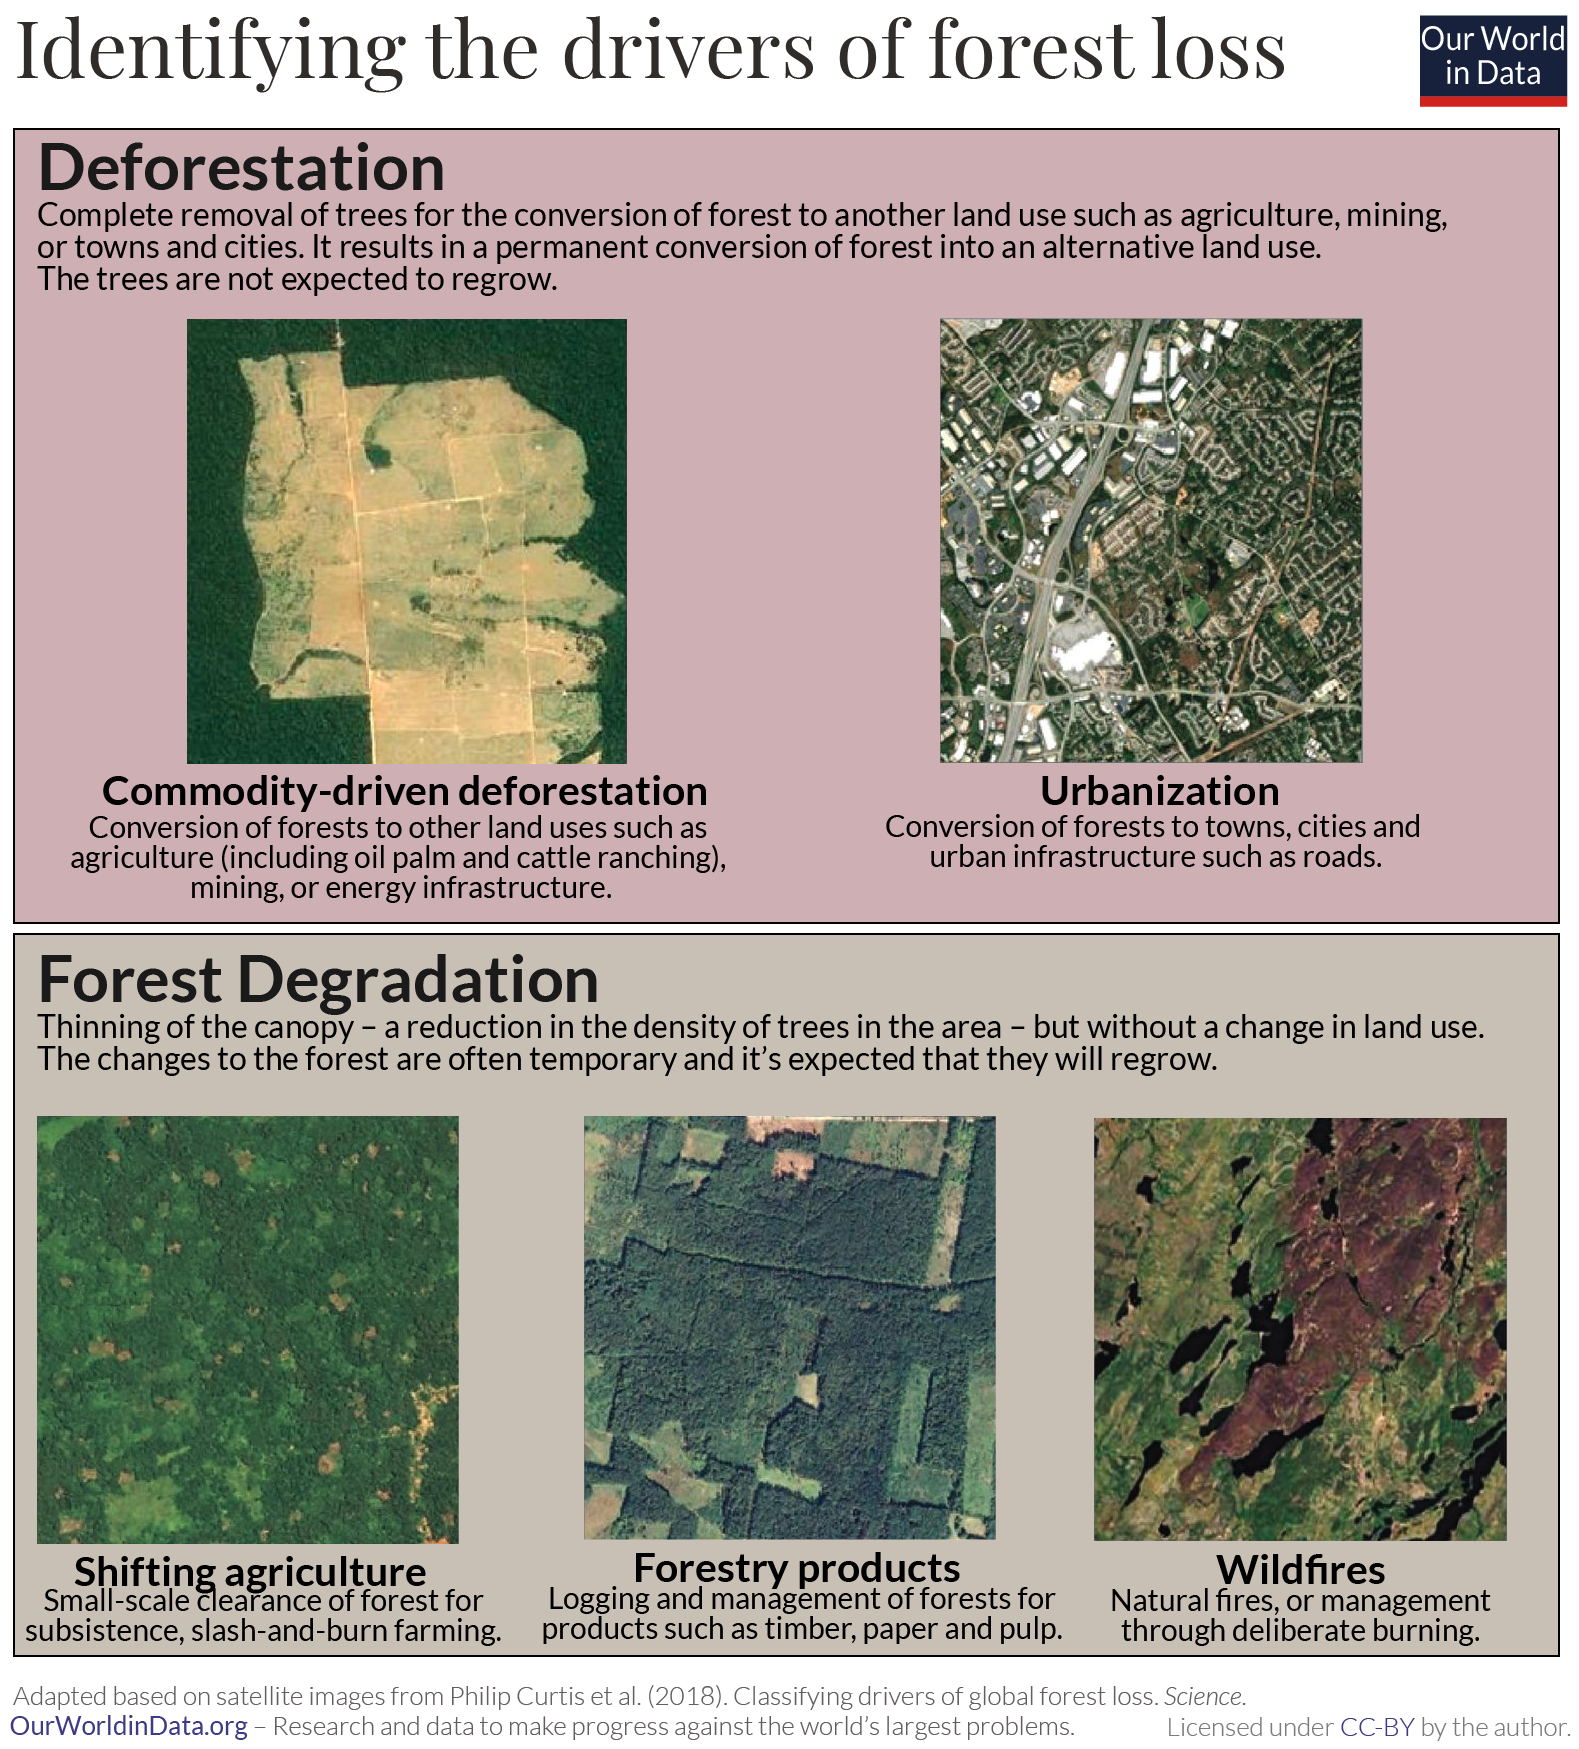
\includegraphics[width=8cm]{imaxes/Identifying-drivers-of-forest-loss.png}
\caption{Gráfico con las principales causas de la perdida de bosques}
\label{fig:drivers of forest lost}
\end{figure}

\section{Objetivos}
\label{sec:Objetivos}

El propósito central de este estudio es llevar a cabo la detección y el conteo de árboles en nubes de puntos LiDAR. La detección se realizará mediante la implementación de algoritmos basados en características geométricas. Estos objetivos principales los podemos desglosar en los siguientes subobjetivos:

\begin{itemize}
    \item Comprender el funcionamiento de la tecnología LiDAR y los datos obtenidos con ella como las nubes de puntos para poder procesar la información en ellas.
    \item Buscar conjuntos de datos adecuados con una cierta densidad de puntos y aprender a utilizar las principales herramientas para el procesamiento y la visualización de nubes de puntos.
    \item Investigar las librerías para procesado de nubes de puntos en \texit{Python}.
    \item Probar diferentes algoritmos y aproximaciones para detectar arboles y estudiar su precisión.
    \item Analizar y Comparar los resultados obtenidos.
\end{itemize}

\section{Apartados de la memoria}
\label{sec:apartados}
La memoria está conformada por los siguientes apartados:
\begin{enumerate}
    \item \textbf{Introducción} : Introduciremos el proyecto y las motivaciones para llevarlo a cabo. Además, se expondrán los objetivos que perseguiremos durante su desarrollo.

    \item \textbf{Fundamentos Teóricos y Tecnológicos} : Se expondrá una breve introducción a la tecnología LiDAR y la forma en que se guardan y procesan los datos obtenidos de esta.
    
    \item \textbf{Metodología} : Comentaremos la metodología elegida para llevar a cabo el trabajo y el por qué de su elección.
    
    \item \textbf{Planificación} : Abordaremos la planificación llevada a cabo para el desarrollo de este proyecto, así como el costo que conllevó su ejecución.
    
    \item \textbf{Detección de árboles basada en estratos} : Se explicará la implementación del algoritmo para la detección de los árboles.
    
    \item \textbf{Análisis de Resultados} : Se probará el algoritmo en diferentes partes del conjunto de datos de Luxemburgo y se estudiarán y analizarán los resultados obtenidos.
    
    \item \textbf{Conclusiones y Trabajo Futuro} : En el capítulo final se presentarán las conclusiones obtenidas en el análisis de los datos y se formularán posibles mejoras que podrían llevarse a cabo en el futuro.


\end{enumerate}


\chapter{Fundamentos Teóricos y Tecnológicos}
\label{chap:fundamentos}

\lettrine{E}{n} este capítulo, se expondrán los fundamentos teóricos y tecnológicos necesarios para comprender este trabajo. Además se comentarán las herramientas en las que nos apoyamos para llevar a cabo esta tarea.

\section{LiDAR}

El término LiDAR se proviene de “Light Detection and Ranging” en inglés. Esta tecnología utiliza un pulsoláser para medir con precisión las distancias y crear una representación tridimensionales de un entorno u objeto.

Su funcionamiento es el siguiente, en un emisor emite un pulso láser hacia una superficie u objeto, mientras que un receptor registra el tiempo que tarda en recibir los rebotes de ese pulso. Esto nos permite obtener con precisión la distancia entre el sensor y el objeto. En nuestro caso al trabajar con datos geoespaciales también es necesario que el sistema esté equipado con un GPS para obtener la ubicación geográfica del sensor.


\begin{figure}[h]
\centering
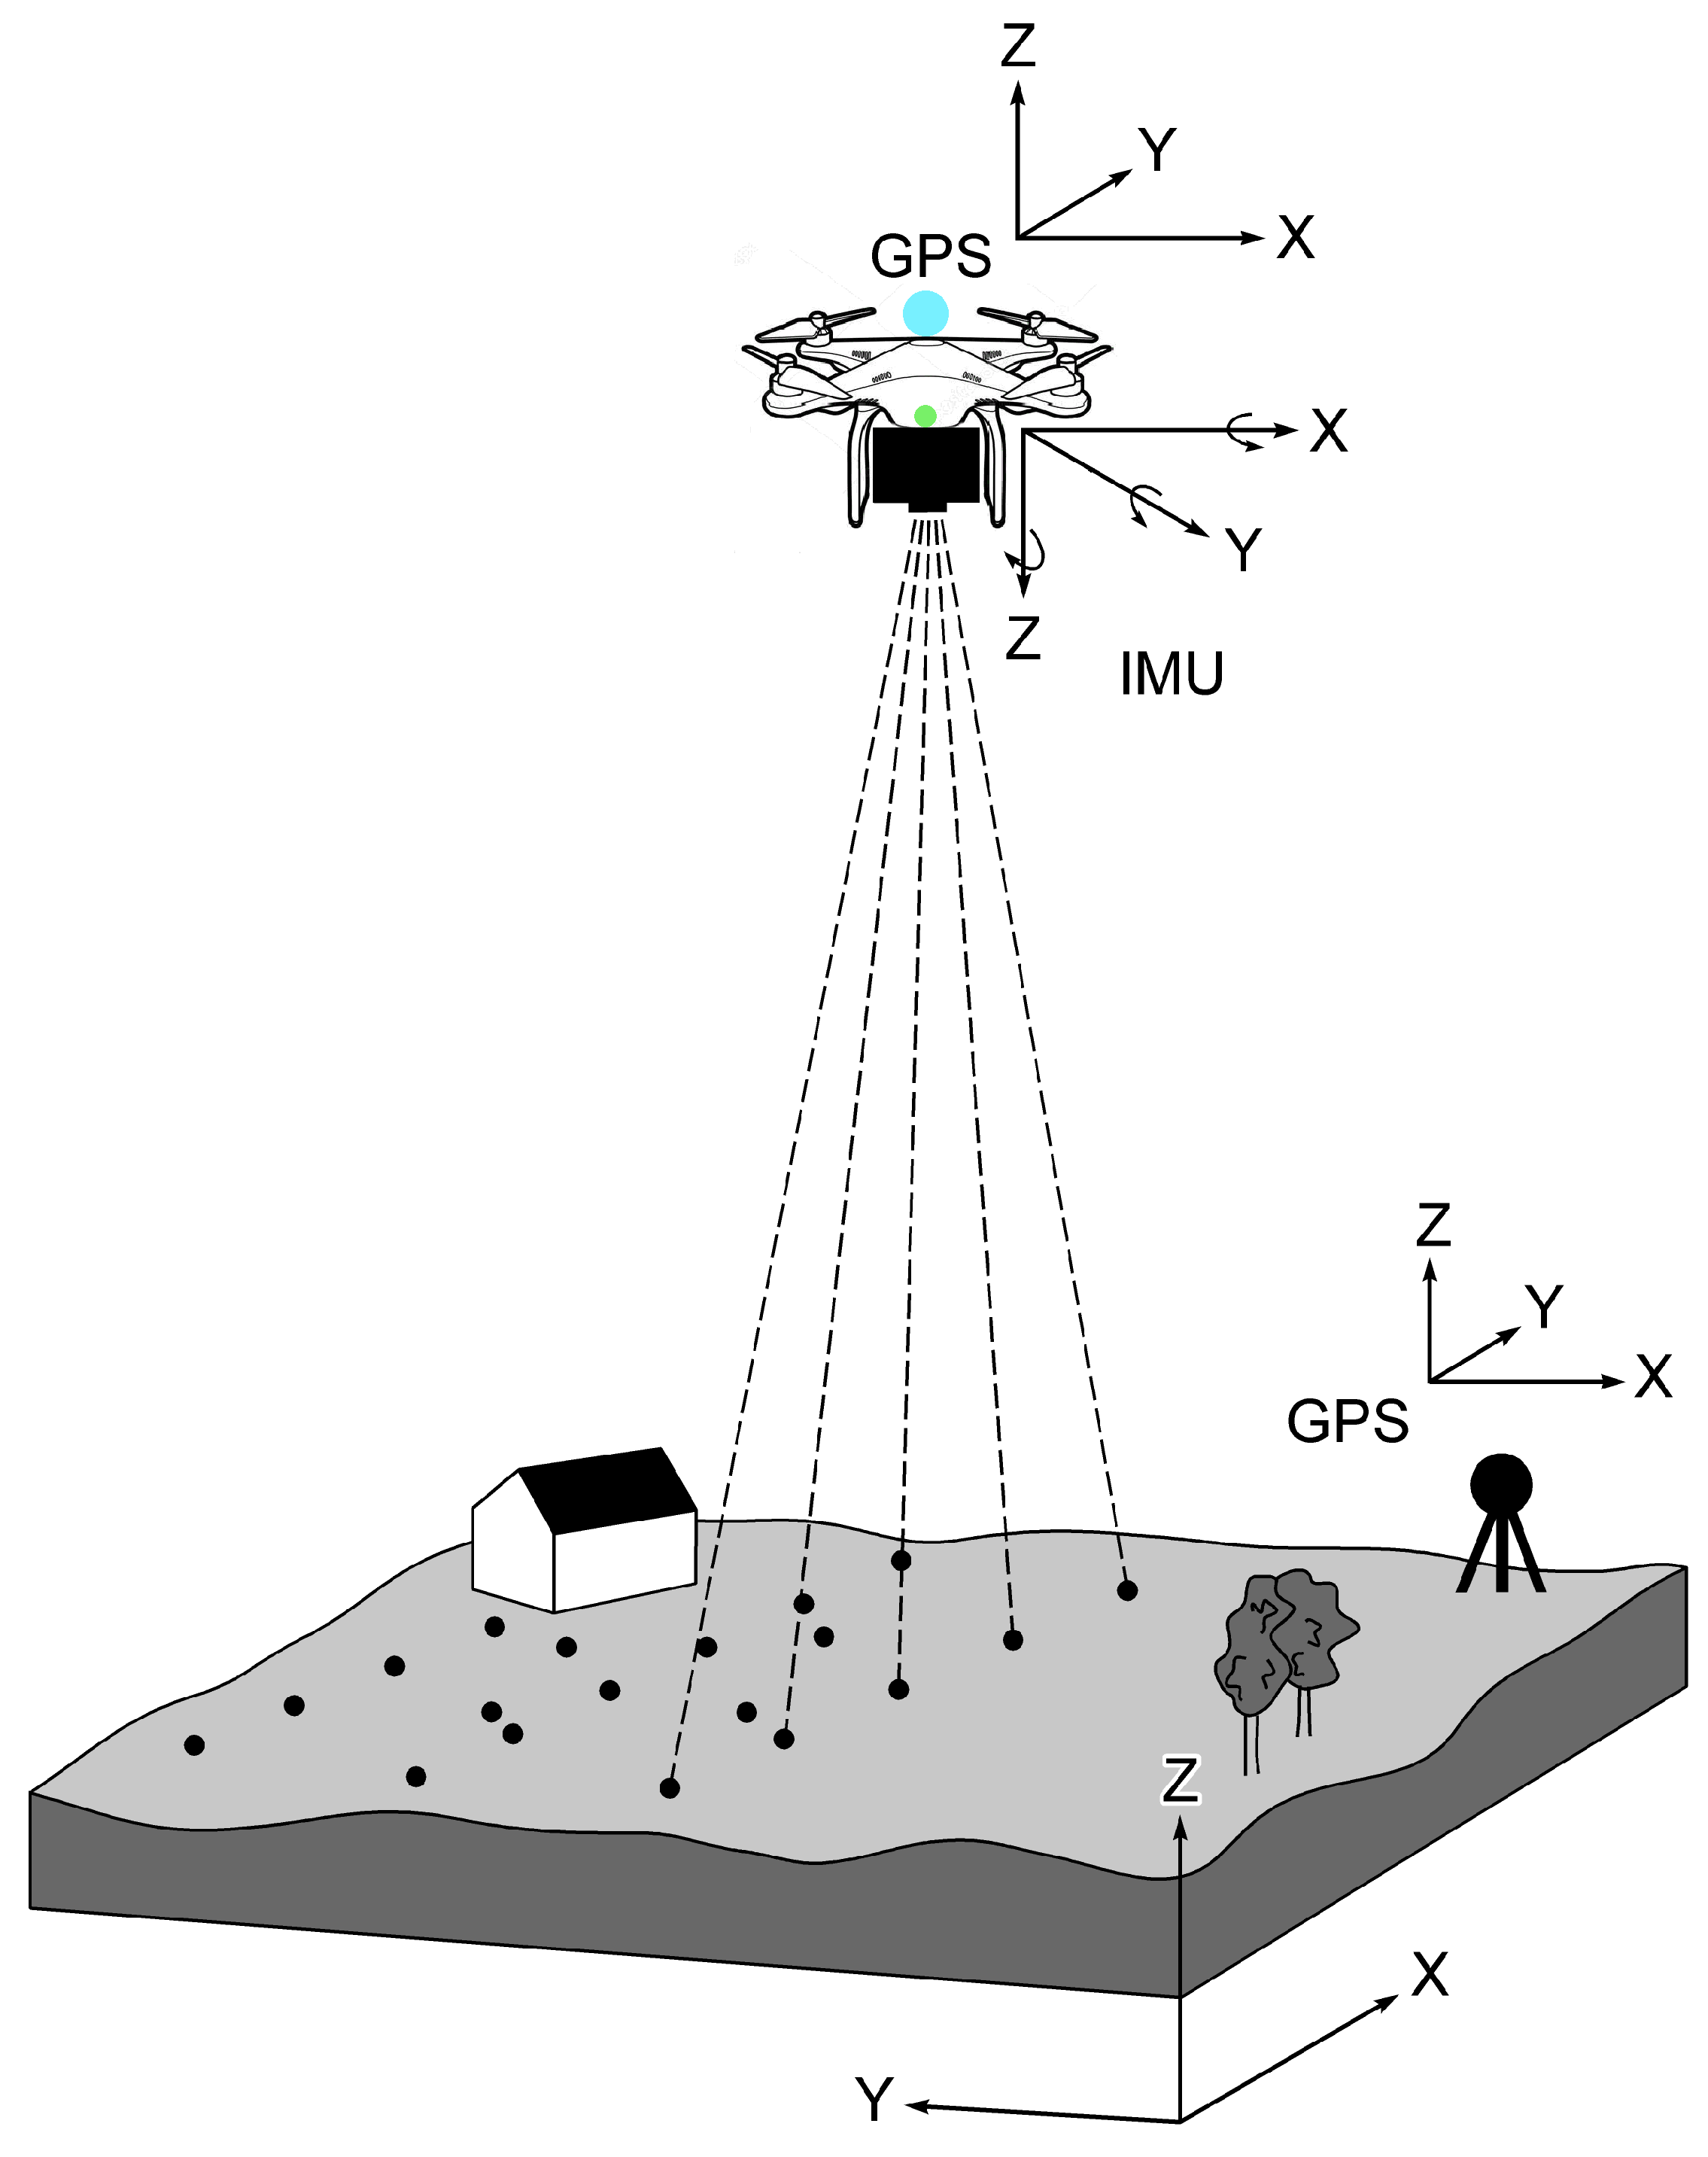
\includegraphics[width=6cm]{imaxes/remotesensing-10-01094-g001.png}
\label{fig:uavsensor}
\caption{Ejemplo de un sistema LiDAR en un UAV \cite{rs10071094}}
\end{figure}


En los últimos años esta tecnología ha experimentado un gran crecimiento debido a su versatilidad y capacidad para ser usado en multitud de escenarios. Entre estos estan el uso en vehículos de conducción autónoma \cite{articleauto}, gestión forestal, como este trabajo, \cite{rs14010170}, para arqueología \cite{lidararque}, agricultura de precision \cite{RIVERA2023107737} o para obtener modelos 3d de ciudades \cite{lidarcity}.

\subsection{Nubes de Puntos}
Las nubes de puntos son el resultado del escaneo de una superficie u objeto, esta nube de puntos no es mas que un conjunto de puntos tridimensionales. Cada uno de estos puntos guarda su coordenada (x, y, z).El par de coordenadas (x, y) representan la ubicación en el plano, y la coordenada (z) la altura de ese punto. Junto con esto también se guardan atributos adicionales para tener mas información de los objetos y superficies. A continuación, explicaremos los más importantes para nuestro trabajo.


\subsubsection{Numero de Retornos}
Existen escenarios en los que un mismo pulso láser puede impactar en superficies con múltiples capas, como ocurre en el caso de un edificio o un árbol. Cada vez que un rayo regresa al sensor, lo denominamos "retorno".

Un símil que puede ayudarnos a comprender mejor esto sería pensar en cuando lanzamos una pelota contra una pared y esta rebota varias veces antes de ser recogida. Cada rebote representaría un "retorno" de la pelota.

En nuestra nube de puntos, registramos cada uno de estos "rebotes" como puntos individuales. Esta información resulta útil para comprender objetos con múltiples capas, como los árboles, que son el objeto de estudio en este trabajo. Específicamente, como veremos más adelante, utilizaremos el primer retorno, ya que en la mayoría de los casos representa la parte superior del árbol, conocida como "corona arbórea".

\subsubsection{Clasificación del objeto}
Cada punto en la nube de puntos puede ser clasificado según su origen. Por ejemplo, si los puntos pertenecen al suelo, edificios o vegetación. Para que esta clasificación sea consistente y homogénea entre todas las nubes de puntos la Sociedad Americana de Fotogrametría y Sensores Remotos (ASPRS) \cite{ASPRS-LAS} propone los siguiente códigos a la hora de clasificar los puntos \ref{tabclas}.

\begin{table}[hp!]
   \centering
  \rowcolors{2}{white}{udcgray!25}
  \begin{tabular}{c|c}
  \rowcolor{udcpink!25}
  \textbf{Valor de clasificación} & \textbf{Significado} \\\hline
  
  0 & Nunca clasificado \\
  1 & No asignado \\
  2 & Terreno  \\
  3 & Vegetación baja  \\
  4 & Vegetación media \\
  5 & Vegetación alta  \\
  6 & Edificio \\
  7 & Punto bajo \\
  8 & Reservado \\
  9 & Agua  \\
  10 & Ferrocarril   \\
  11 & Superficie de la carretera   \\
  12 & Reservado   \\
  13 & Protector de cable (señal)   \\
  14 & Conductor de cable (fase)   \\
  15 & Torre de transmisión   \\
  16 & Conector de la estructura de cables (aislante)   \\
  17 & Plataforma del puente \\
  18 & Ruido alto \\
  19-63 & Reservado \\
  64-255 & Definido por el usuario 

  \end{tabular}

  \caption{Códigos de clasificación LAS definidos por ASPRS para las versiones LAS 1.1 a 1.4}
  \label{tabclas}


\end{table}

\subsubsection{Densidad de puntos}
Este valor representa la cantidad de puntos en una región específica, lo que puede proporcionar detalles sobre la complejidad del objeto o la resolución del escaneo. Para este proyecto, es importante tener regiones con altas densidades de puntos para ser capaces de reconocer la estructura del árbol, tanto la copa como el tronco.

\vspace{0.5cm}

Una vez comprendido qué conforma una nube de puntos, necesitamos entender cómo se guardan estos datos. El formato más ampliamente utilizado es el LAS (LiDAR Data Exchange Format), desarrollado por la ya mencionada Sociedad Americana de Fotogrametría y Sensores Remotos. Este formato es altamente eficiente y permite diferentes niveles de compresión. Al ser el formato más extendido, será el más utilizado por las herramientas de procesamiento y visualización.

Como alternativa a este formato, y también muy utilizado, tenemos el LAZ, un formato que utiliza técnicas de compresión sin pérdida para reducir el tamaño del archivo sin perder precisión. Normalmente, los datos LAS se pueden convertir a LAZ sin ningún problema y posteriormente, para su procesamiento, se pueden volver a descomprimir.

\section{Detección de Objetos}

La detección de objetos en nubes de puntos es una tarea crucial en diversas aplicaciones como la conducción autónoma, la planificación urbana o la robótica. Existen varias aproximaciones para realizar esto, cada una de con sus ventajas y limitaciones. Ahora expondremos algunas de las técnicas más comunes usadas en este ámbito:

\subsection{Segmentación basada en Clústeres}

La segmentación basada en clústeres agrupa puntos que están cerca unos de otros en clústeres, lo que permite identificar regiones que probablemente representen objetos o partes del entorno. Métodos como el crecimiento de regiones, K-means, Mean Shift y DBSCAN son ampliamente utilizados para esta técnica. La segmentación basada en clústeres es efectiva para detectar objetos con formas y tamaños variados.

\begin{figure}[h]
\centering
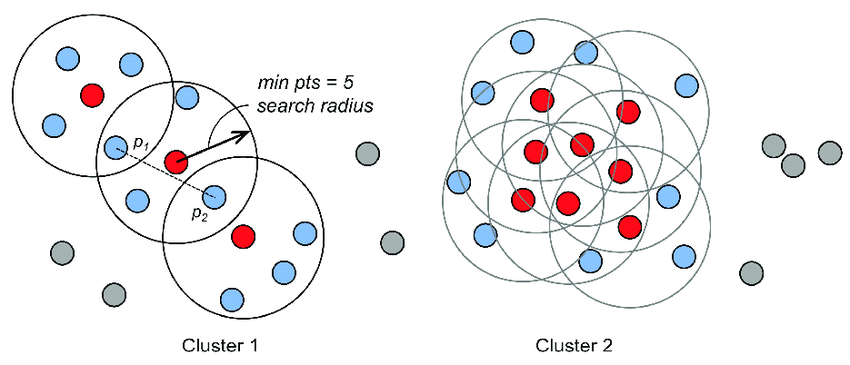
\includegraphics[width=10cm]{imaxes/The-DBSCAN-algorithm-and-two-generated-clusters-There-are-three-types-of-points-as.png}
\label{fig:pointnetc}
\caption{Ejemplo del funcionamiento del algoritmo de clustering \textit{dbscan} \cite{dbscan}}
\end{figure}


\subsection{Extracción de Características}

La extracción de características implica la identificación de atributos significativos de los puntos en una nube, como la altura, la intensidad del retorno, la densidad de puntos y la distribución espacial. Estos atributos se utilizan para identificar regiones que podrían contener objetos. Esta técnica es muy versátil y puede combinarse con otras para mejorar los resultados.


\subsection{Aprendizaje Automático (Machine Learning)}

El aprendizaje automático, como el uso de redes neuronales convolucionales (CNN) y métodos de aprendizaje profundo, permite a los sistemas aprender patrones complejos directamente de los datos. Los modelos se entrenan con datos etiquetados y luego se utilizan para detectar objetos en nuevas nubes de puntos. Esta técnica es eficaz para capturar relaciones no lineales y características sutiles.

\begin{figure}[h]
\centering
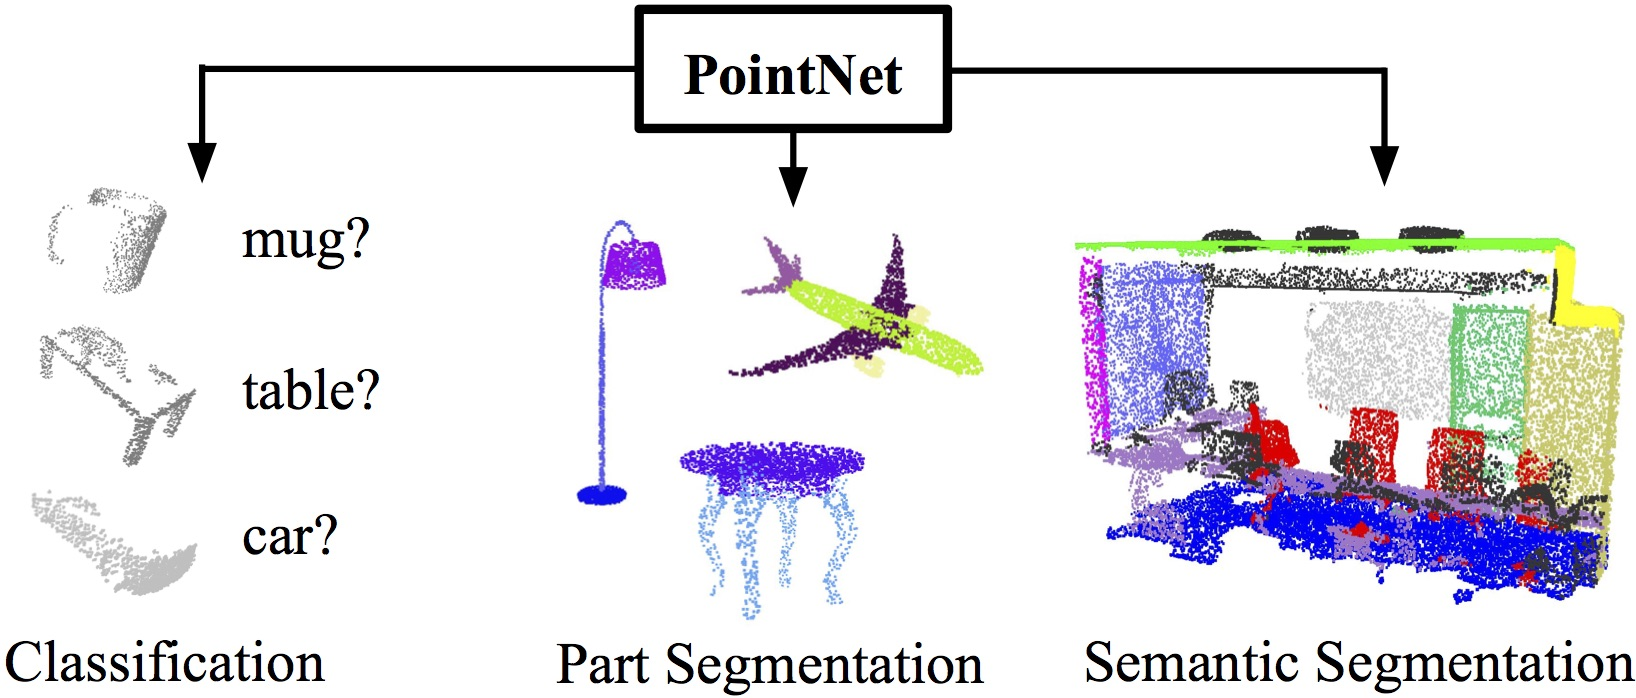
\includegraphics[width=10cm]{imaxes/teaser.jpg}
\label{fig:pointnetc}
\caption{Ejemplo de la red PointNet \cite{pointnet}}
\end{figure}


\subsection{Filtros Geométricos}
Los filtros geométricos son técnicas que eliminan puntos que no pertenecen a objetos sólidos, como el suelo o elementos del entorno. Filtros como el de plano y el de distancia se emplean para mantener solo los puntos relevantes para la detección de objetos.


\subsection{Análisis de Vecinos Cercanos}

El análisis de vecinos cercanos implica evaluar la distribución y proximidad de los puntos en la nube. Los puntos con suficientes vecinos cercanos en un área se consideran parte de un objeto o una superficie. Esta técnica es efectiva para detectar regiones densas y agrupaciones de puntos.


\section{Herramientas}
Para el procesado de nubes de puntos es necesario utilizar herramientas para visualizar y tratar los datos. En la mayoría de los lenguajes de programación tenemos disponibles bibliotecas o librerías que nos lo permiten, como por ejemplo, PDAL, de la cual hablaremos más adelante.
A continuación se presentaran las herramientas empleadas durante el desarrollo del trabajo.

\subsection{QT Reader}
Esta es una herramienta gráfica muy sencilla que nos permite visualizar nubes de puntos con una interfaz simple, concisa y veloz. Esta herramienta nos permite utilizar los formatos más comunes, como LAS o LAZ.

\begin{figure}[h]
\centering
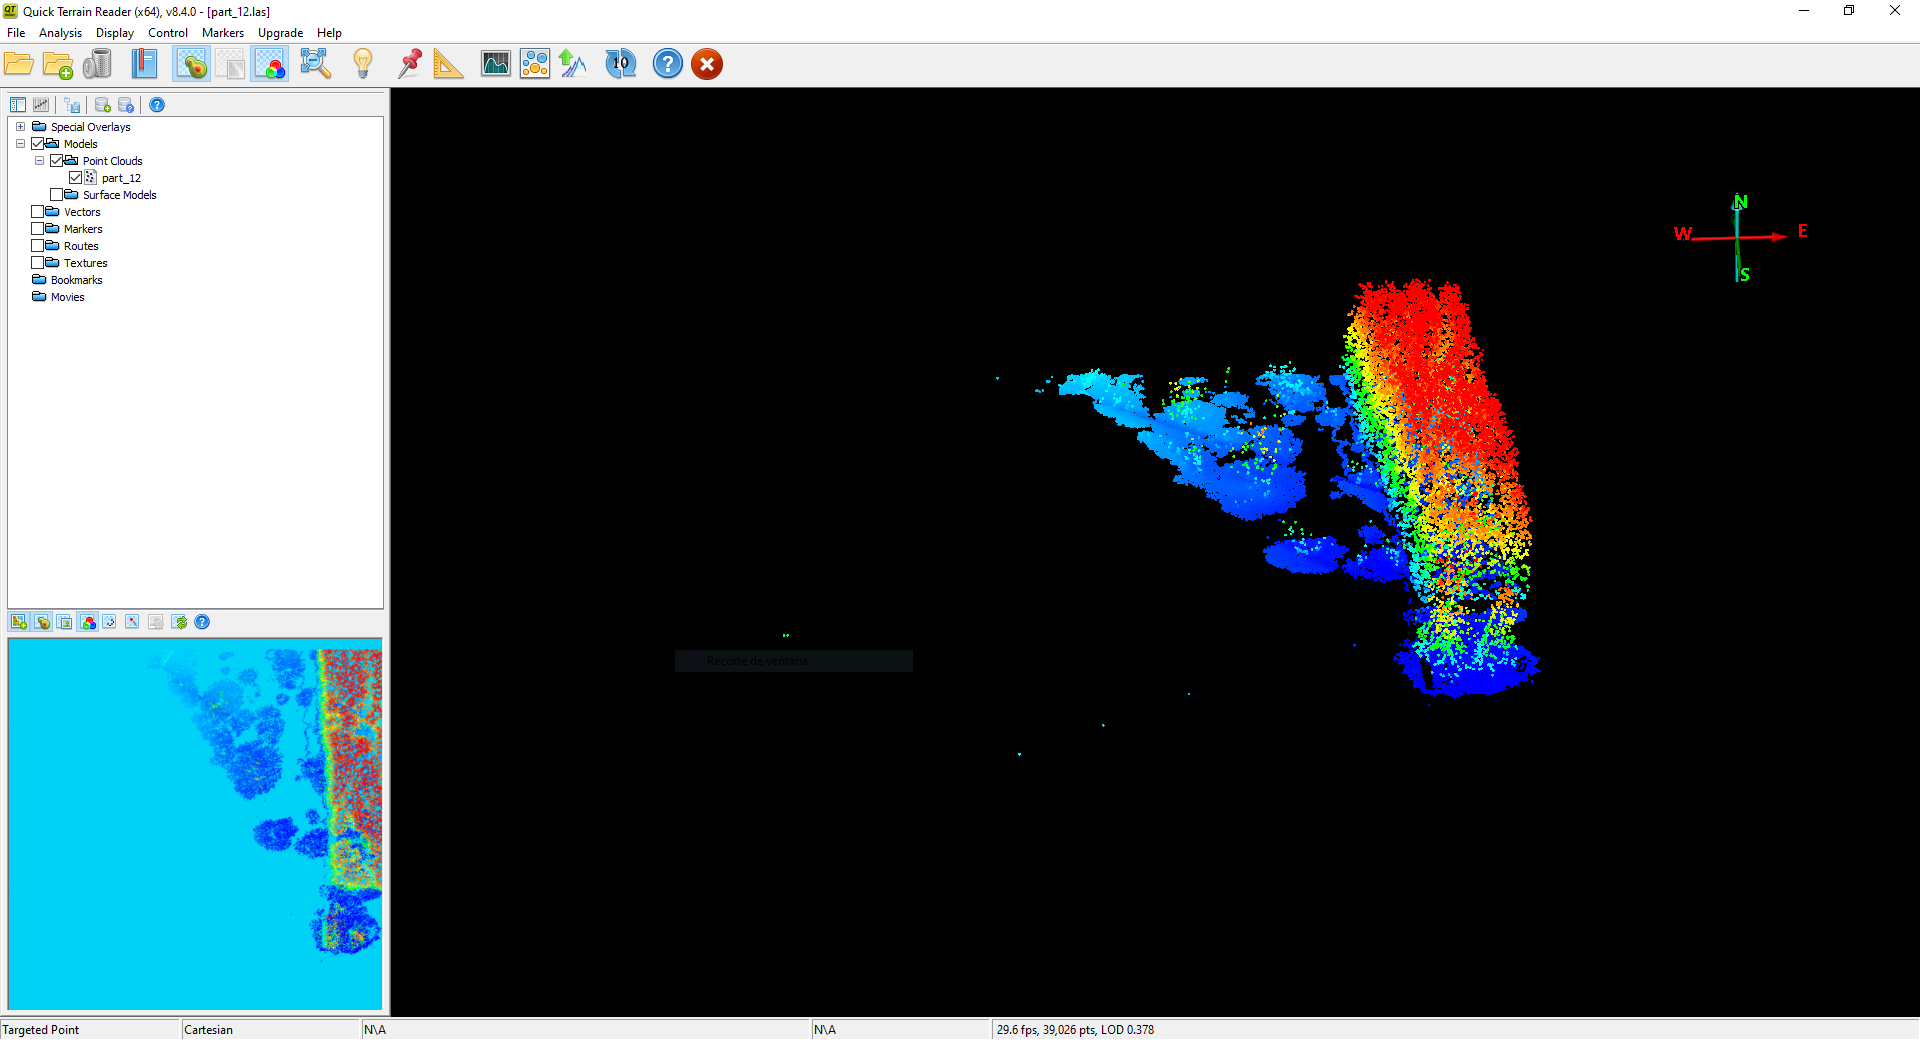
\includegraphics[width=10cm]{imaxes/qtreaderventana.png}
\label{fig:pointnetc}
\caption{Interfaz de QR Reader}
\end{figure}

\subsection{PADL}

PDAL (Point Data Abstraction Library) es una biblioteca de código abierto desarrollada en C++ para procesar y analizar datos de nubes de puntos en 3D. Nos permite leer, escribir, filtrar y transformar datos en los principales formatos. Además, cuenta con bibliotecas que permiten su utilización en varios lenguajes diferentes \cite{pdal}.

\subsection{Open3D}
Es otra biblioteca de código abierto para el procesamiento y visualización de nubes de puntos. En este proyecto, se utilizó debido a las herramientas que ofrece para la visualización interactiva de las nubes de puntos \cite{Open3d}.

\subsection{WhiteBox Tools}
Esta es una herramienta para el procesamiento de nubes de puntos que consta de diversos algoritmos diseñados para el procesamiento de datos LiDAR \cite{Whitebox}.

\subsection{Python}
Es un lenguaje de alto nivel muy flexible, con una amplia variedad de bibliotecas disponibles tanto para el procesamiento de datos LiDAR como para matemáticas. Este es el lenguaje sobre el cual se basa toda nuestra implementación \cite{python}.

\subsection{Conda}
Es un gestor de paquetes y un sistema de administración de entornos para lenguajes como Python. Permite instalar y gestionar paquetes; en nuestro caso, se usó para hacer uso de PDAL \cite{conda}.



\chapter{Metodología}
\label{chap:metodologia}

\lettrine{E}{n} este capítulo se expondrá la metodología elegida. En nuestro caso, optamos por una metodología incremental ágil con una gestión del flujo de trabajo mediante Kanban.

\section{Introducción a la metodología}

Para este proyecto se termino optando por la metodología ágil \cite{scrum}. En concreto, se optó por un enfoque basado en un desarrollo incremental, donde la gestión del flujo de trabajo se realizó con Kanban.


Este enfoque incremental permite desarrollar pequeños incrementos que van mejorando y puliendo las funcionalidades de nuestro sistema de forma progresiva. Esta metodología se adapta muy a entornos donde los requisitos no están de todo claros en el principio y en el futuro son susceptibles a cambios. Este es el caso de un trabajo de fin de grado donde normalmente se empieza con una idea pero no se sabe muy bien como abordar el problema desde un principio, por lo que tener esta flexibilidad para hacer cambios conforme avance el proyecto y recibamos retroalimentación es muy útil. 

La Gestión de Flujo de Trabajo Kanban se implementó empleando un tablero visual en la plataforma Notion. Esta metodología facilitó una gestión eficiente del flujo de trabajo al proporcionar una representación visual de las tareas, organizadas en categorías de pendientes, en progreso y completadas. Además es muy fácil realizar ajustes en estas tareas según la retroalimentación recibida en las reuniones.


\begin{figure}[h]
\centering
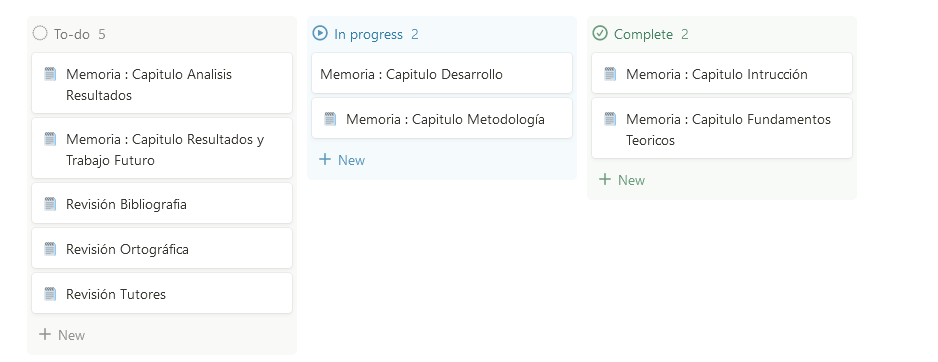
\includegraphics[width=14cm]{imaxes/kanban.png}
\label{fig:pointnetc}
\caption{Ejemplo de Kanban para el desarrollo de la memoria}
\end{figure}


\section{Desarrollo Incremental}

Previamente se introdujo el desarrollo incremental, ahora lo comentaremos con más detalle.
Este desarrollo se basa en la premisa de que es más efectivo y adaptable desarrollar algo en partes pequeñas y simples en vez de abordar el proyecto en su totalidad de una sola vez. Cada incremento se desarrolla en un período de tiempo determinado con un grupo de funcionalidades. Esto nos permite obtener retroalimentación temprana para saber si nos estamos desviando y ajustarnos al resultado que buscamos. Además, al desarrollar en partes pequeñas se reduce el riesgo de desarrollar algo incorrecto y darnos cuenta al final.

\subsection{Incrementos}

Los incrementos son unidades de trabajo que representan un conjunto de funcionalidades entregables. Cada incremento agrega nuevas funcionalidades o corrige las anteriores, y está diseñado para ser funcional por sí mismo. Al final de cada incremento, en nuestro caso, era revisado con los tutores del trabajo, y se discutían las futuras líneas de trabajo sobre él, así como la forma en que podríamos mejorar lo hecho hasta ahora.


\begin{figure}[h]
\centering
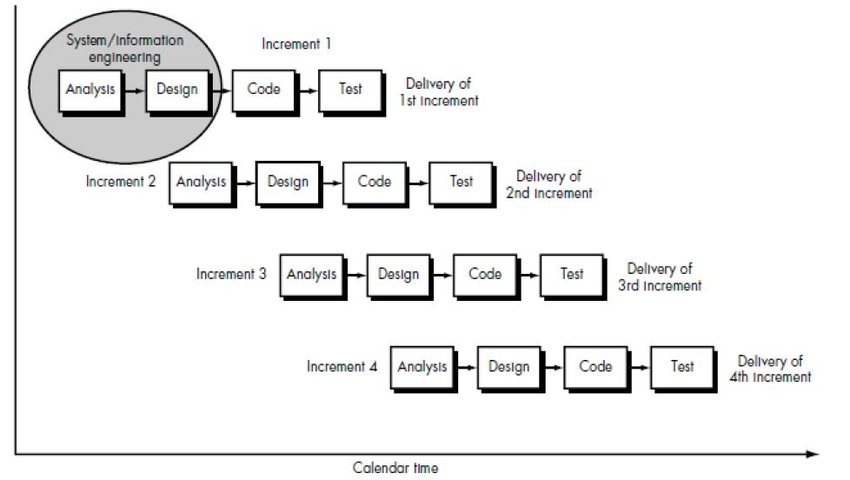
\includegraphics[width=12cm]{imaxes/Incremental-software-development-model.png}
\label{fig:pointnetc}
\caption{Ejemplo de un desarrollo incremental \cite{inproceedings}}
\end{figure}



\chapter{Planificación}
\label{chap:planification}

\lettrine{U}{n}a vez comentada la metodología a usar, discutiremos cómo se llevó a cabo la planificación de nuestro proyecto. A continuación, presentaremos y analizaremos las diferentes iteraciones que conformaron dicha planificación.

\section{Iteración 1 : Investigación y Preparación Inicial}
\label{chap:investigPlan}

En esta primera iteración partimos desde cero, aún no tenemos nada construido. Esta etapa tuvo una duración de una semana, del 9 al 16 de mayo de 2023.

Primero se realizaron búsquedas de publicaciones sobre la detección de árboles en nubes de puntos. Durante esta fase, nos encontramos con la publicación \cite{rs15061619}, de la cual obtuvimos la idea de utilizar máximos como un enfoque inicial. También destacamos la publicación de \textit{Forest Ecosystems} \cite{ZHANG2023100088}, de la cual tomamos la idea de utilizar las secciones del tronco. Además, en paralelo, comenzamos la búsqueda de repositorios de nubes de puntos. En esta búsqueda tuvimos en cuenta la densidad de puntos, ya que era fundamental poder identificar el tronco ya que en densidades bajas no se pueden ver. Finalmente, después de considerar varias opciones optamos por utilizar el repositorio de Luxemburgo.


Después de informarnos y revisar las aproximaciones ya existentes procedimos a realizar pruebas con la herramienta \textit{WhiteBox Tools} para evaluar diferentes algoritmos destinados a la modificación de nubes de puntos, tales como la eliminación del suelo o la reducción de ruido. Una vez completada esta iteración, concluyó con una reunión con los tutores durante la cual se discutió la información obtenida y se propusieron nuevos objetivos para la próxima iteración.

\section{Iteración 2 : Preparación del entorno de Desarrollo}
En esta segunda fase se comenzó a buscar el entorno y los lenguajes que se utilizarían para desarrollar el trabajo. Durante esta etapa se comenzó barajando la opción de usar el lenguaje \textit{Rust} debido a su gran eficiencia. El problema radica en que aprender este lenguaje en poco tiempo es algo complejo y las bibliotecas disponibles para el procesamiento de nubes de puntos son escasas y tienen poca documentación, por lo que esta opción se descartó.

La otra opción que se barajó fue \textit{Python}. Dado que es un lenguaje más extendido en el mundo del procesamiento de datos y lleva más tiempo en el mercado, ofrece una amplia variedad de herramientas tanto para modificar como para visualizar nubes de puntos. La mayor desventaja de este enfoque es que es un lenguaje de muy alto nivel que, en términos de rendimiento, puede ser el doble de lento a \textit{Rust}. Para solucionarlo inconveniente, existen bibliotecas que permiten llamar a funciones escritas en otro lenguaje, como \textit{C++}, desde nuestro código de \textit{Python}. Un ejemplo de esto es PDAL, que nos permite utilizar el pipeline de procesamiento de nubes de puntos escrito en \textit{C++} desde \textit{Python} o \textit{Conda}. Finalmente, esta fue la opción por la que se optó. Informamos a los tutores de esta decisión y procedimos a la instalación de \textit{Conda} para utilizar PDAL. Esta tarea abarcó desde el 16 de mayo al 23 de mayo de 2023.


\section{Iteración 3 : Desarrollo de una primera versión}
En esta Iteración se procedió a desarrollar una primera versión capaz de convertir la nube de puntos 3d en un matriz 2d que represente la altura de cada punto y a partir de esta matriz obtener los máximos que nos servirán como un punto de partida en la detección.
La primera tarea será convertir ese conjunto de datos 3D en una matriz 2D. Una vez con esta matriz procederemos a buscar los máximos locales dentro de un umbral de vecindad. Esta tarea tomo desde el 23 de mayo hasta el 6 de junio, para terminarla se reunió con los tutores se les presento las nuevas funcionalidades y se propusieron mejoras para una próxima Iteración. 

\section{Iteración 4 : Desarrollo de una  usando Estratos }
En esta fase se desarrollara el algoritmo que comentamos en la sección \ref{chap:Deteccion}. Partiremos de los máximos locales obtenidos previamente para buscar en ellos características que puedan confirmar que es un árbol. En nuestro caso se optó por coger los puntos dentro de una sección cilíndrica con centro en el máximo y radio un parámetro que configuraremos en el código, y partiendo de esos puntos usar técnicas como RANSAC o obtener los centroides de diferentes secciones para determinar si es un árbol o no. A mayores de esto para esta parte de análisis de características se le pasará la nube de puntos con alturas normalizadas y sin suelo, esto lo obtendremos gracias al pipeline de PDAL.

Lo último que se realizó en esta iteración fue que se seleccionaron unos tiles de prueba y se les asignó un clasificación con la localización de los puntos, para hacer esta tarea se desarrolló una pequeña utilidad que guarde los puntos que nosotros marcamos manualmente como árboles en un \textit{CSV}. A partir de estos tiles podremos ir obteniendo unas primeras métricas para ver que tan preciso es nuestro sistema. Esta tarea abarca desde el 7 de junio al 2 de julio.

\section{Iteración 5 : Mejora del Sistema de Centroides}
Anteriormente se creó un sistema para obtener el centroide de diferentes secciones del estrato y comprobar la linealidad, si el valor obtenido era mayor de cierto umbral se clasificaba ese punto como un árbol. En esta iteración se planteo y desarrolló un sistema para que en cada sección se aplique un algoritmo de clustering y obtener el centroide de cada cluster.Esto se decidió hacer así por que previamente la aparición de ramas podaría dar resultado a un falso negativo. Con este nuevo sistema tendremos un árbol con todos los centroides y al recorrer todas las secciones buscaremos en esa estructura de datos el mejor conjunto de centroides, esto lo veremos de manera más detallada en el capitulo \ref{chap:Deteccion}.

A mayores de esto se comenzó a realizar la memoria, en concreto la parte relacionada con el algoritmo comentado previamente.
La realización de esta iteración comenzó el 3 de julio y termino el 17 de ese mismo mes.

\section{Iteración 6 : Pruebas y análisis de los test}
Una vez con el sistema desarrollado se paso a la obtención de los tiles y su preparación para realizar pruebas. Se eligieron solo tiles de Luxemburgo y de diferentes zonas forestales con diferentes tipos de árboles. Sobre estes se realizaron pruebas y se ejecutaron los algoritmos, con los resultados obtenidos se guardaron y se analizaron posteriormente para incluir los resultados obtenidos en la memoria. Esta tarea comenzó el 17 de julio y terminó el 23 de julio.

\section{Iteración 7 : Realización de la Memoria}

En esta última fase con toda la información obtenida a lo largo del desarrollo del proyecto se realizó el desarrollo de la memoria. Se crearon grafismos y diagramas con el fin de que los lectores entiendan mejor el funcionamiento. Para la realización del diagrama de gantt para mostrar la planificación de la memoria se opto por usar la herramienta de código abierto \textit{Mermaid.js} que nos permite la creación de estes mediante código y css. Esta última iteración comenzó el 23 de julio hasta el 10 de septiembre.


\section{Costes}
Una vez con la planificación hecha realizaremos una estimación de los costes de este proyecto. Primero establecemos el coste de los recursos humanos.El coste por hora de un desarrollador junior son aproximadamente 9€/h \cite{saljun} y el coste promedio de dos profesores doctorados por hora es de 18€/h \cite{saldoc}. El tiempo total lo obtendremos de la planificación y suponemos que se trabajan 3 horas al día y las reuniones con los tutores son de 2h. El coste total lo vemos en la tabla \ref{tabcospes}

\begin{table}[hp!]
   \centering
  \rowcolors{2}{white}{udcgray!25}
  \begin{tabular}{c|c|c|c}
  \rowcolor{udcpink!25}
  \textbf{Nombre del Recurso} & \textbf{Coste por hora} & \textbf{Horas Trabajadas} & \textbf{Total}\\\hline
  
  Programador Junior & 9 €/h & 420 h & 3780 € \\
  Tutor 1 & 18 €/h & 18 h & 324 € \\
  Tutor 2 & 18 €/h & 18 h & 324 €  \\
  \textbf{Total}  & & & \textbf{4428 €}\\

  \end{tabular}

  \caption{Tabla con el desglose de los costes humanos}
  \label{tabcospes}


\end{table}

  Ahora nombraremos los costes materiales, en esta parte contaremos tanto los recursos físicos como el ordenador como el coste de las licencias del software usado. Primero empezaremos por el ordenador, estos tienen un ciclo de vida de entre 6 a 10 años y su costo fue de 900 €, si el proyecto duró 4 meses y la vida media la definimos en 7 años el coste por mes sería de sobre 11 € al mes. Para el desarrollo se uso el IDE \textit{Pycharm} de la empresa \textit{JetBrains}  que tiene un coste de 24.99 € al mes \cite{costjet}.

\begin{table}[hp!]
   \centering
  \rowcolors{2}{white}{udcgray!25}
  \begin{tabular}{c|c|c|c}
  \rowcolor{udcpink!25}
  \textbf{Nombre del Recurso} & \textbf{Coste Mensual} & \textbf{Meses de Uso} & \textbf{Total}\\\hline
  
  Ordenador & 11 €/mes & 4 meses & 44 € \\
  Licencia Pycharm & 24.99 €/mes & 4 meses & 99.96 € \\
  \textbf{Total}  & & & \textbf{143.96 €} \\
  \end{tabular}

  \caption{Tabla con el desglose de los costes materiales}
  \label{tabcospes}
\end{table}

Con todo esto en la figura \ref{tabcostot} vemos el coste total del proyecto.

\begin{table}[hp!]
   \centering
  \rowcolors{2}{white}{udcgray!25}
  \begin{tabular}{c|c}
  \rowcolor{udcpink!25}
  \textbf{Nombre del Recurso} & \textbf{Coste} \\\hline
  
  Costes Humanos & 4428 € \\
  Costes Materiales & 143.96 €  \\
  \textbf{Total}  &  \textbf{4571.96 €} \\
  \end{tabular}

  \caption{Tabla con el coste total}
  \label{tabcostot}
\end{table}


\begin{figure}[h]
\centering
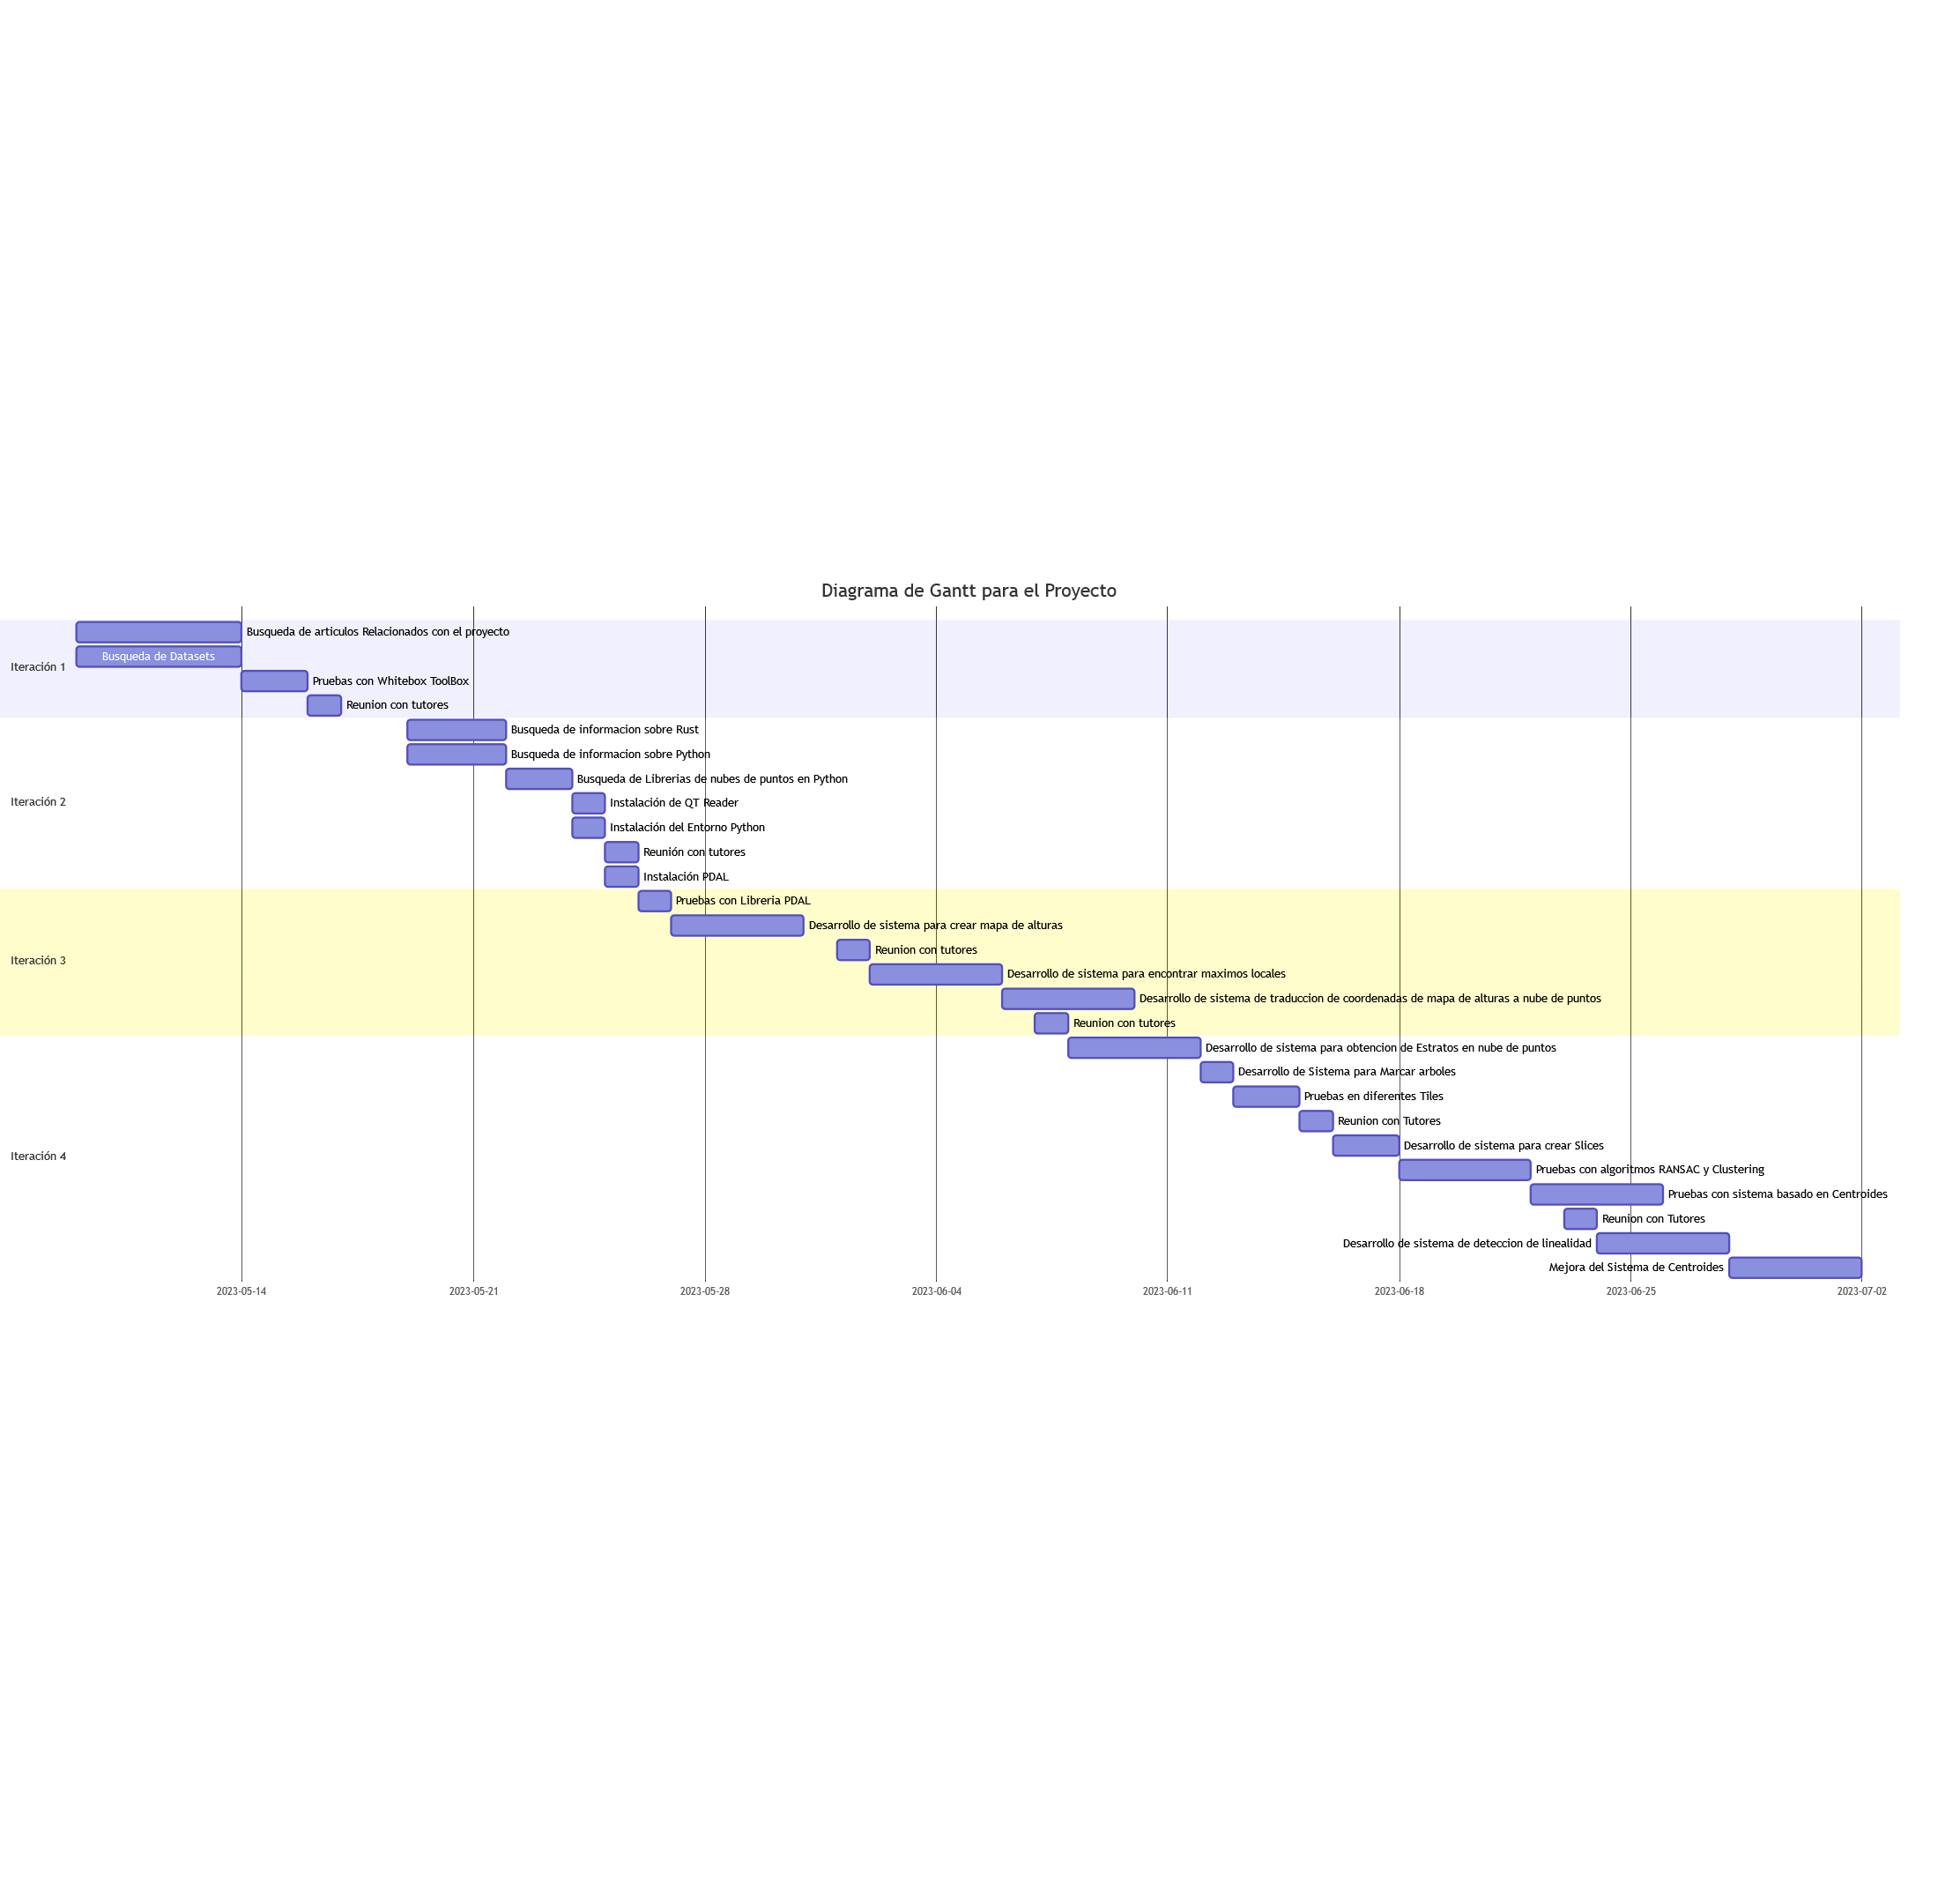
\includegraphics[width=15cm]{imaxes/gantt1.png}
\label{fig:pointnetc}
\caption{Primeras 4 iteraciones del Diagrama de Gantt}
\end{figure}

\begin{figure}[h]
\centering
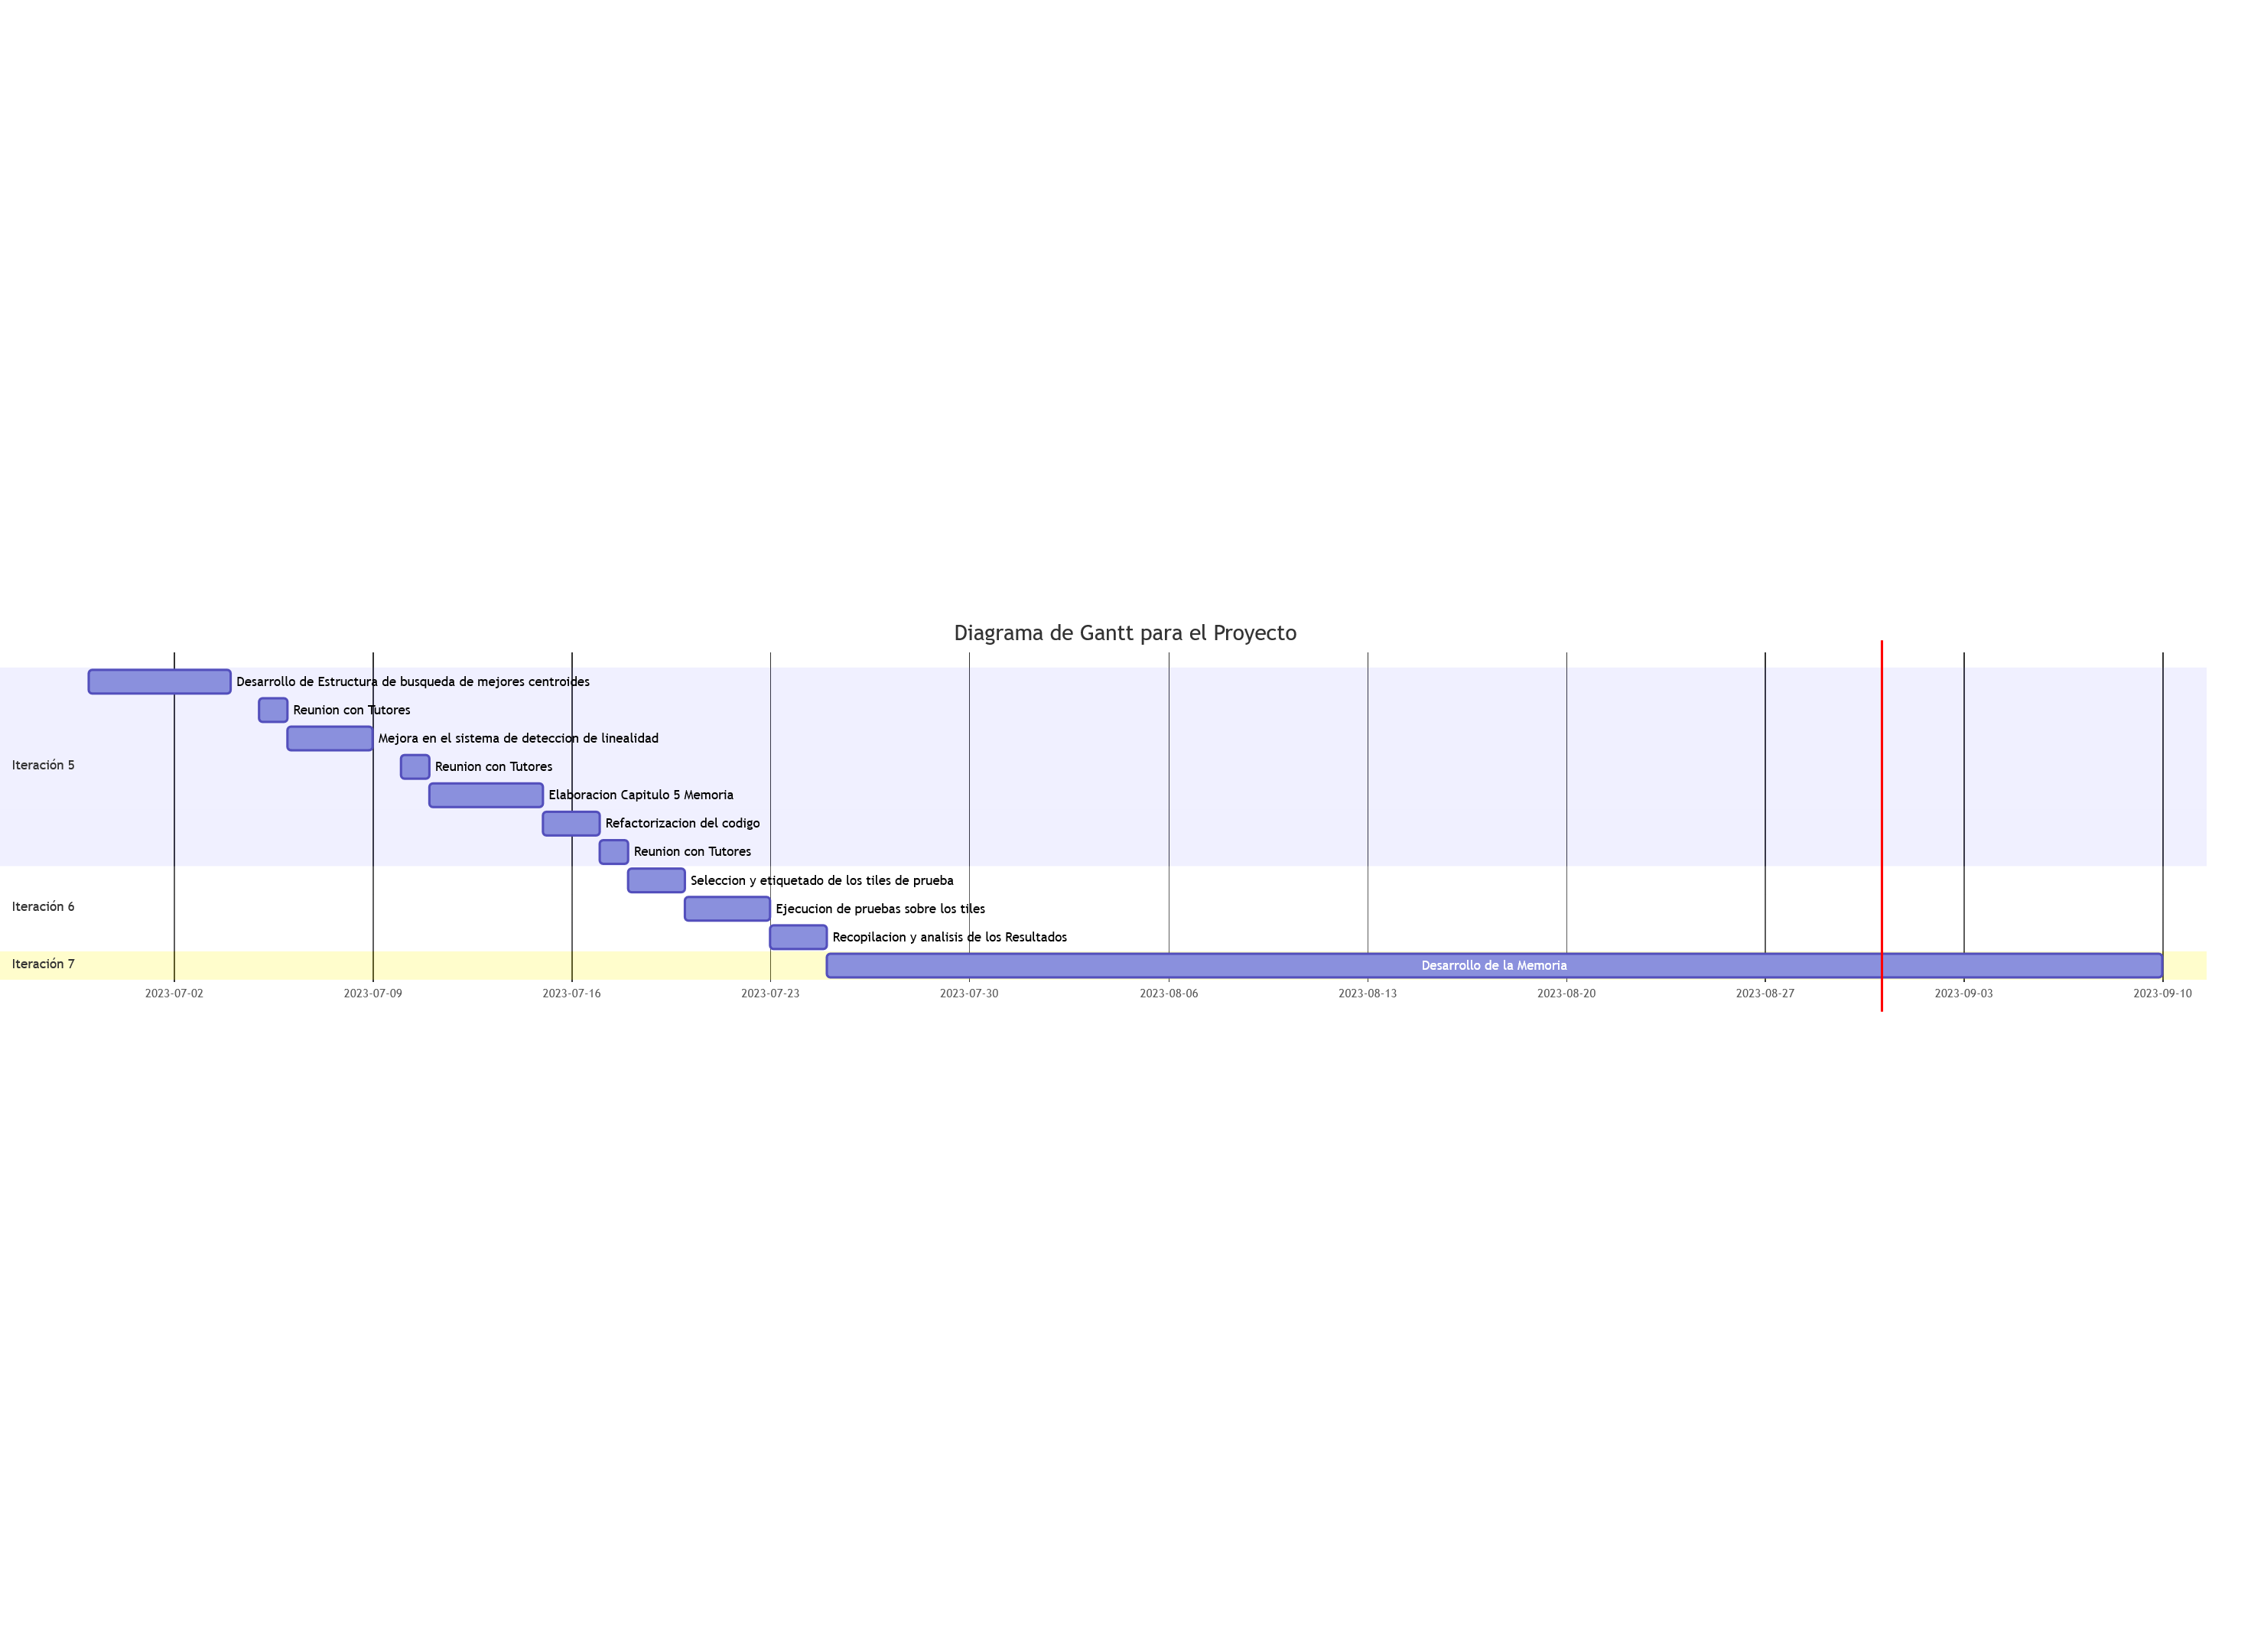
\includegraphics[width=15cm]{imaxes/gantt2.png}
\label{fig:pointnetc}
\caption{Últimas iteraciones del Diagrama de Gantt}
\end{figure}


\chapter{Detección de árboles basada en estratos}
\label{chap:Deteccion}
Este capítulo se dedicará a explicar el algoritmo planteado para la detección de árboles en Nubes de Puntos. La figura \ref{fig:diagFlujoAlgoritmo} representa el diagrama de flujo del algoritmo empleado para la detección de árboles, cada fase de este tendrá una sección dedicada a él explicando a fondo su funcionamiento.

\section{Estructura del Algoritmo}
\label{sec:EstrucuturaProp}

\begin{figure}[h]
\centering
\includegraphics[height=8.5cm]{imaxes/flujoalgo.png}
\caption{Diagrama de Flujo del Algoritmo}
\label{fig:diagFlujoAlgoritmo}
\end{figure}


\subsection{Obtención de las Alturas Normalizadas}
\label{chap:normalAlgo}

La obtención de las alturas normalizadas, también conocidas como alturas sobre el suelo (HAG), es un paso esencial para la detección y análisis de objetos elevados como árboles en nubes de puntos. Las alturas normalizadas eliminan la elevación del terreno y se centran en la altura relativa de los objetos con respecto a la superficie del suelo.
Esto nos ayuda a reducir errores provocados por los diferentes desniveles del terreno y nos ayuda a la comparación de los resultados entre diferentes regiones ya que nos concentramos únicamente en la verticalidad de los puntos que conforman los árboles.

\begin{figure}[h]
  \begin{subfigure}{0.5\textwidth}
    \centering
    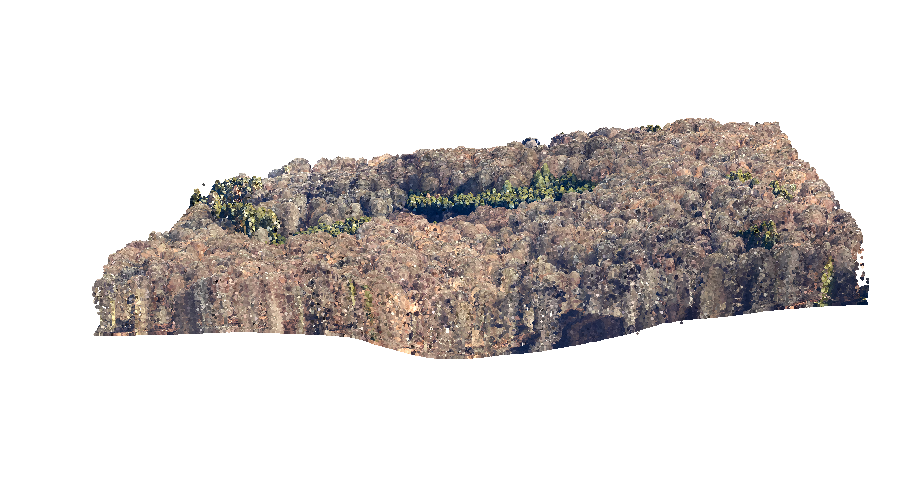
\includegraphics[width=0.8\linewidth]{imaxes/nohag.png}
    \caption{Nube de puntos sin alturas normalizadas}
    \label{fig:sub1}
  \end{subfigure}%
  \begin{subfigure}{0.5\textwidth}
    \centering
    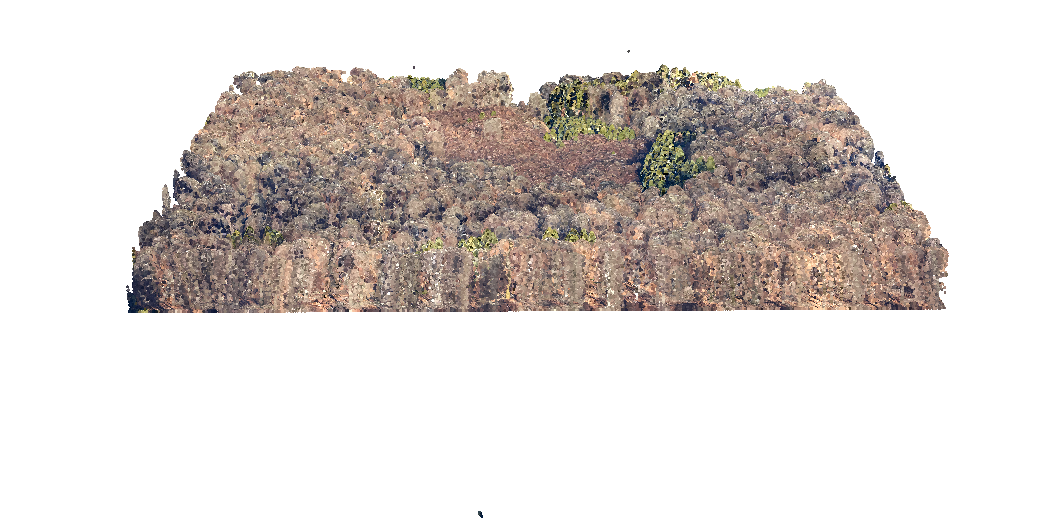
\includegraphics[width=0.8\linewidth]{imaxes/hag.png}
    \caption{Nube de puntos con alturas normalizadas}
    \label{fig:sub2}
  \end{subfigure}
  \label{fig:algo1}
\end{figure}

\subsection{Obtención del Last Return}
\label{chap:LastAlgo}

Esta parte es fundamental en este algoritmo. El uso del último retorno en la detección de árboles mejora la visualización y la caracterización del tronco, debido a que este retorno sufre menos interferencia de la vegetación y ruido. Al alcanzar la cima del árbol, proporciona una visión directa del tronco sin obstrucciones de las hojas y ramas superiores. Esto permite una identificación más precisa de la altura, forma y detalles del tronco, siendo esencial en aplicaciones como análisis de árboles.

\subsection{Eliminación del suelo}
\label{chap:groundAlgo}
En esta fase, el objetivo es eliminar los puntos que corresponden al suelo, ya que no son necesarios para la detección y su inclusión solo requeriría un mayor consumo de recursos. Para este paso, se utilizó el algoritmo basado en simulación de ropa de Zhang, el cual está disponible en PDAL \cite{rs8060501}.

El método CSF crea una malla virtual que abarca toda la nube de puntos y luego ajusta dicha malla a los puntos de la nube. A cada punto se le estima la altura de la malla mediante la interpolación de los puntos dentro de cada triángulo. Luego, se identifican los puntos que constituyen ruido al comparar la altitud de los puntos de la nube con la altitud estimada en la malla.

Esta aproximación nos permite filtrar los datos de manera sencilla, sin requerir una gran cantidad de parámetros, y proporciona resultados precisos.

\begin{figure}
  \begin{subfigure}{0.5\textwidth}
    \centering
    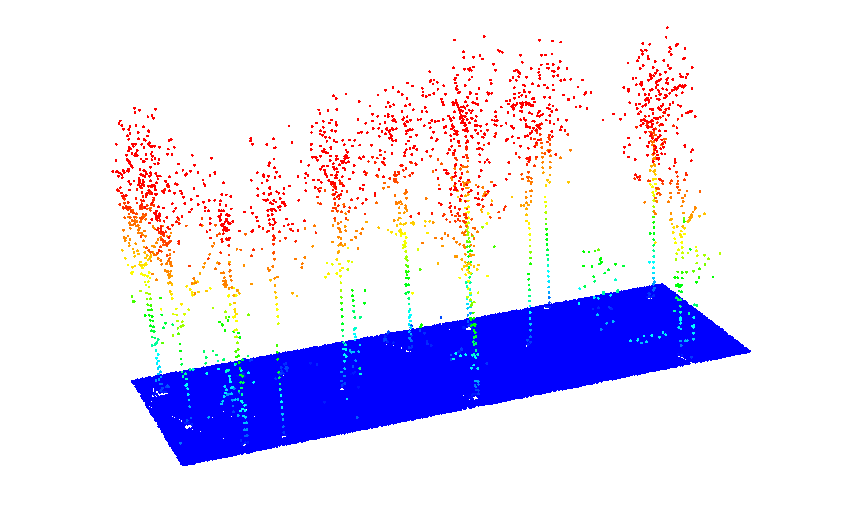
\includegraphics[width=0.8\linewidth]{imaxes/last.png}
    \caption{Nube de puntos con los últimos retornos}
    \label{fig:last1}
  \end{subfigure}%
  \begin{subfigure}{0.5\textwidth}
    \centering
    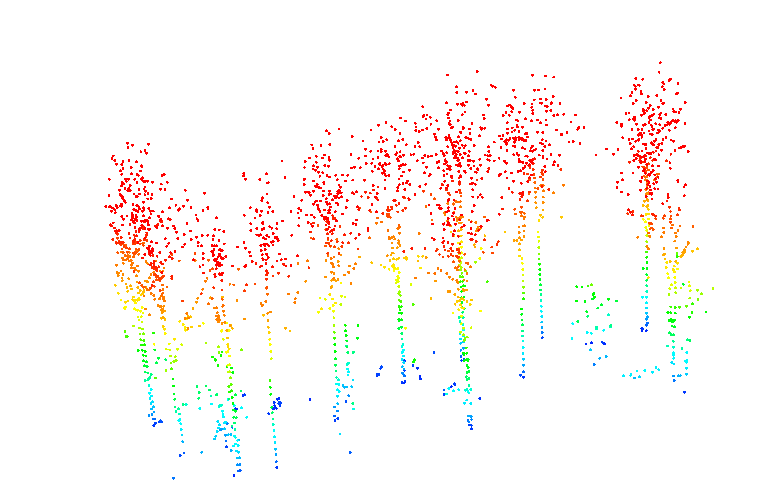
\includegraphics[width=0.8\linewidth]{imaxes/lastnog.png}
    \caption{Nube de puntos con últimos retornos sin suelo}
    \label{fig:last}
  \end{subfigure}
  \label{fig:algo2}
\end{figure}



\subsection{Creación de un Mapa de Alturas}
El mapa de alturas es una matriz 2D que representa la altura del dosel de los árboles en función de las coordenadas espaciales X e Y.

En primer lugar, se determinan las coordenadas mínimas y máximas del modelo de nube de puntos. Esto proporciona el rango espacial en el que se encuentra la nube de puntos.

A continuación, se crea una cuadrícula regular con una resolución especificada. Esta cuadrícula se forma mediante una serie de puntos espaciados de manera uniforme en el rango determinado por las coordenadas mínimas y máximas.

Luego, se construye un árbol KD (KD-tree) a partir del modelo de nube de puntos. Un árbol KD es una estructura de datos que permite realizar búsquedas eficientes de vecinos más cercanos.

Después de tener la cuadrícula y el árbol KD, se procede a realizar una consulta a los vecinos más cercanos para cada punto de la cuadrícula. Esto implica encontrar el punto más cercano en el modelo de nube de puntos para cada punto de la cuadrícula.

Una vez obtenidos los vecinos más cercanos, se recupera la altura del dosel correspondiente a cada punto en relación con el suelo. Esto se logra obteniendo las alturas asociadas a los puntos encontrados en la consulta previa.

Finalmente, los valores de altura del dosel se organizan en un mapa de alturas, donde cada punto de la cuadrícula tiene asignada una altura del dosel correspondiente. Este mapa se usará en la próxima etapa para obtener los puntos donde potencialmente se encuentra un árbol.

Se podría pensar que una forma más rápida de obtener este mapa de alturas sería coger simplemente la altura de cada punto en la nube, pero el problema de esto es que las nubes son irregulares y existen partes donde hay más densidad de puntos que en otras, donde los puntos muestreados tendrán una distribución no uniforme. Con el fin de tener una representación fiel y precisa, optamos por usar un \textit{KD-tree} y sacrificar un poco de rendimiento.

En el ejemplo \ref{fig:chmexample} podemos ver cómo a partir de una nube de puntos, obtenemos su mapa de alturas.

\vspace{0.2cm}
\begin{lstlisting}[language=Python, caption={Código para obtener el mapa de alturas del dosel}]
def compute_canopy_height_model(point_cloud_height_model, resolution):
    min_coords_height_model = np.min(point_cloud_height_model, axis=0)
    max_coords_height_model = np.max(point_cloud_height_model, axis=0)

    x_grid = np.arange(min_coords_height_model[0], max_coords_height_model[0], resolution)
    y_grid = np.arange(min_coords_height_model[1], max_coords_height_model[1], resolution)
    xx, yy = np.meshgrid(x_grid, y_grid)
    xy_flat = np.column_stack((xx.ravel(), yy.ravel()))

    kdtree = cKDTree(point_cloud_height_model[:, :2])

    _, indices = kdtree.query(xy_flat, k=1)

    canopy_height = point_cloud_height_model[indices, 2]

    canopy_height_model = canopy_height.reshape(xx.shape)
    return canopy_height_model
\end{lstlisting}


\subsection{Detección usando Máximos}

Haciendo uso del mapa de alturas obtenido antes, aplicando un umbral y un tamaño de filtro específico se pueden identificar los puntos que tienen potencial de ser árboles.

En primer lugar se realiza un filtrado de máximo local en el mapa de alturas. Este proceso consiste en examinar cada punto y determinar si es el valor máximo dentro de un vecindario definido por el tamaño de filtro establecido. La distancia de búsqueda del máximo local está determinada por el tamaño del vecindario. Esto lo podemos ver como la variable \textit{filter\_size} en la implementación \ref{lst:detectT} y con \textit{threshold}, ambos valores son definidos previamente como constantes.

A continuación, se crea una máscara que identifica los puntos en el mapa de alturas que cumplen dos condiciones: deben ser iguales a los máximos locales encontrados y deben ser mayores que el umbral establecido. 
Por último, se obtienen los índices correspondientes a los puntos que cumplen las condiciones establecidas en la máscara. Estos índices representan las ubicaciones de los árboles detectados en el mapa de alturas.

\vspace{0.2cm}
\begin{lstlisting}[language=Python, caption={Código para la busqueda de máximos }, label=lst:detectT]
def detect_trees_in_max(canopy_height_model, threshold, filter_size):

    neighborhood_size = (filter_size, filter_size)
    local_max = maximum_filter(canopy_height_model, footprint=np.ones(neighborhood_size), mode='constant')
    tree_mask = (canopy_height_model == local_max) & (canopy_height_model > threshold)
    tree_indexes = np.where(tree_mask)
    
    return tree_indexes
\end{lstlisting}

La figura \ref{fig:chm_max} muestra los puntos máximos dentro del mapa de alturas obtenido previamente.

\begin{figure}[h]
\centering
\begin{subfigure}[t]{.4\textwidth}
  \centering
  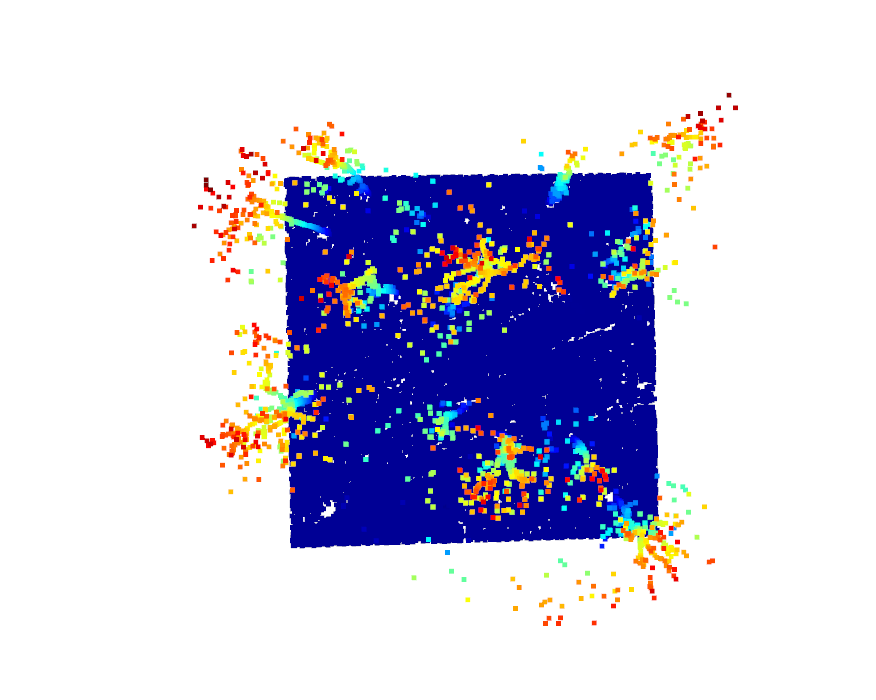
\includegraphics[height=6cm]{imaxes/slice_sup.png}
  \caption{Nube de puntos Original desde arriba}
  \label{fig:slice_top}
\end{subfigure}
\begin{subfigure}[t]{.4\textwidth}
  \centering
  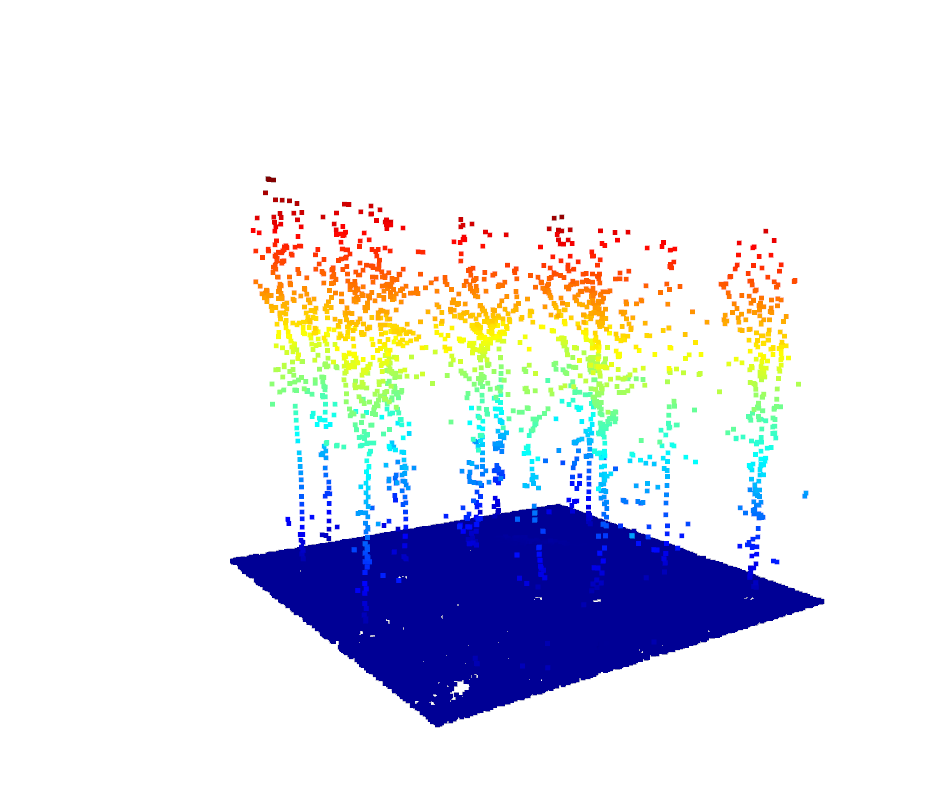
\includegraphics[height=6cm]{imaxes/slice_lat.png}
  \caption{Nube de puntos original vista lateral}
  \label{fig:slice_lat}
\end{subfigure}
\begin{subfigure}[t]{.4\textwidth}
  \centering
  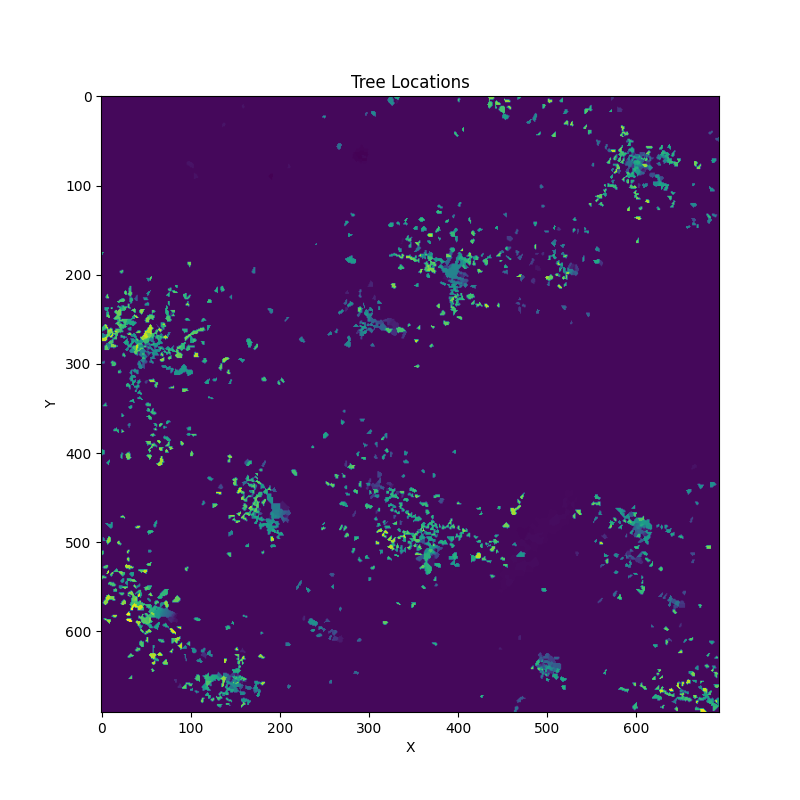
\includegraphics[height=6cm]{imaxes/chm.png}
  \caption{Mapa de alturas}
  \label{fig:chm}
\end{subfigure}%
\begin{subfigure}[t]{.4\textwidth}
  \centering
  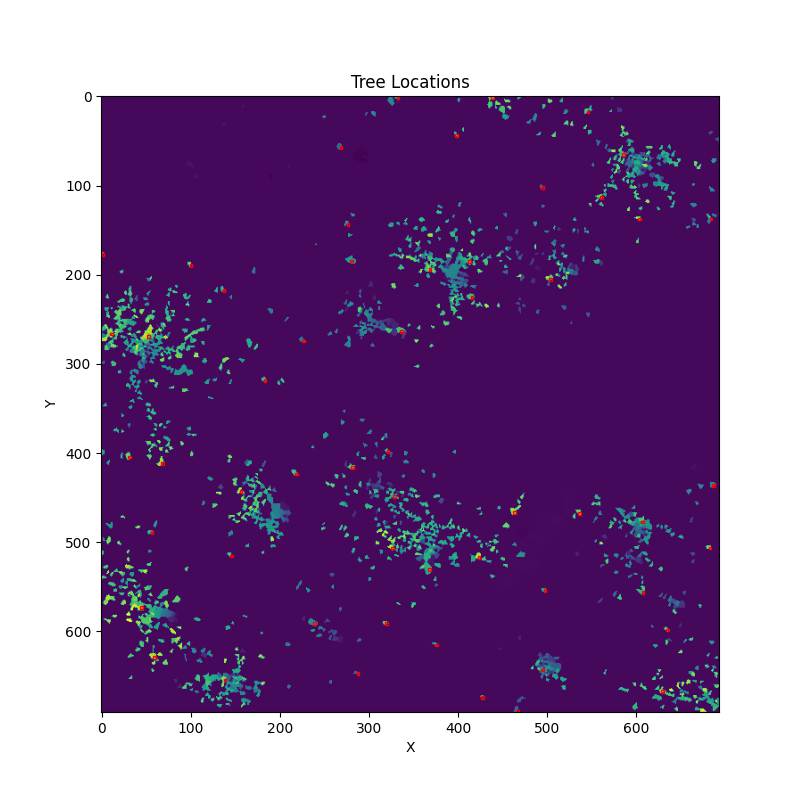
\includegraphics[height=6cm]{imaxes/chm_with_trees.png}
  \caption{Mapa de alturas con los máximos}
  \label{fig:chm_max}
\end{subfigure}

\caption{Ejemplo de obtención de árboles mediante máximos}
\label{fig:chmexample}
\end{figure}

\subsection{Detección de árboles mediante árboles de búsqueda}

Una vez obtenidos los puntos con potencial de ser árboles, obtendremos una sección cilíndrica de puntos con centro en ese punto. Esta sección tiene un radio que determinaremos, y dentro de ella se tienen que encontrar los puntos que conforman ese \textit{árbol}.

Los troncos de los árboles tienden a tener una estructura que forma una línea, aunque en ciertas especies, llegada cierta altura, comienza a tener muchas ramificaciones.

Lo que buscamos es ser capaces de encontrar esa linealidad en esa sección. Para eso, la partiremos en \textit{slices} de la misma altura y obtendremos el centroide. Las slices tendrán un tamaño fijo que definimos previamente. Un centroide representa el centro geométrico de los puntos de esa rodaja. Con una lista de estos, obtendremos una calificación en función de que también se ajuste a una línea, y en función de si es mayor a un umbral o no, se determinará si es realmente un árbol.

Para obtener este valor de que tan bien se ajustan a una linea usaremos el método de los mínimos cuadrados. Este método busca minimizar la suma de los cuadrados de las diferentes ordenadas. La ecuación de una línea en 3D se representa como $z = ax + by + c$, donde $z$ es la coordenada vertical y $x$ e $y$ son las coordenadas horizontales. Los coeficientes $a$, $b$, y $c$ se determinan para minimizar la función de error:

\[
E(a, b, c) = \sum_{i=1}^{n} (z_i - (ax_i + by_i + c))^2
\]
donde $n$ es el número de puntos y $(x_i, y_i, z_i)$ son las coordenadas de cada punto. La optimización se realiza para encontrar los valores de $a$, $b$, y $c$ que minimizan esta función, lo que permite construir la ecuación de la línea que mejor se ajusta a los datos.

Si nuestro algoritmo solo tuviera en cuenta eso podrían surgir problemas al encontrarse con ramificaciones o con puntos que aun que estén dentro del cilindro pueden ser de otro árbol o ruido. 
Con el fin de hacer el algoritmo más robusto, antes de calcular el centroide de cada slice, se aplica un algoritmo al conjunto de puntos que la conforman, en concreto uno de \textit{clustering}, en nuestro caso usamos DBSCAN, que se basa en la agrupación en la densidad de puntos en una zona. En una primera implementación, en el caso de tener más de un centroide en una slice podríamos seleccionar solo el que se ajuste mejor a una recta con los centroides previos, pero con esta decisión estaríamos descartando centroides que aunque en el contexto de esa sección se ajustan peor, en el contexto de todo el árbol pueden tener un mejor ajuste.

\begin{figure}[h]
\centering
    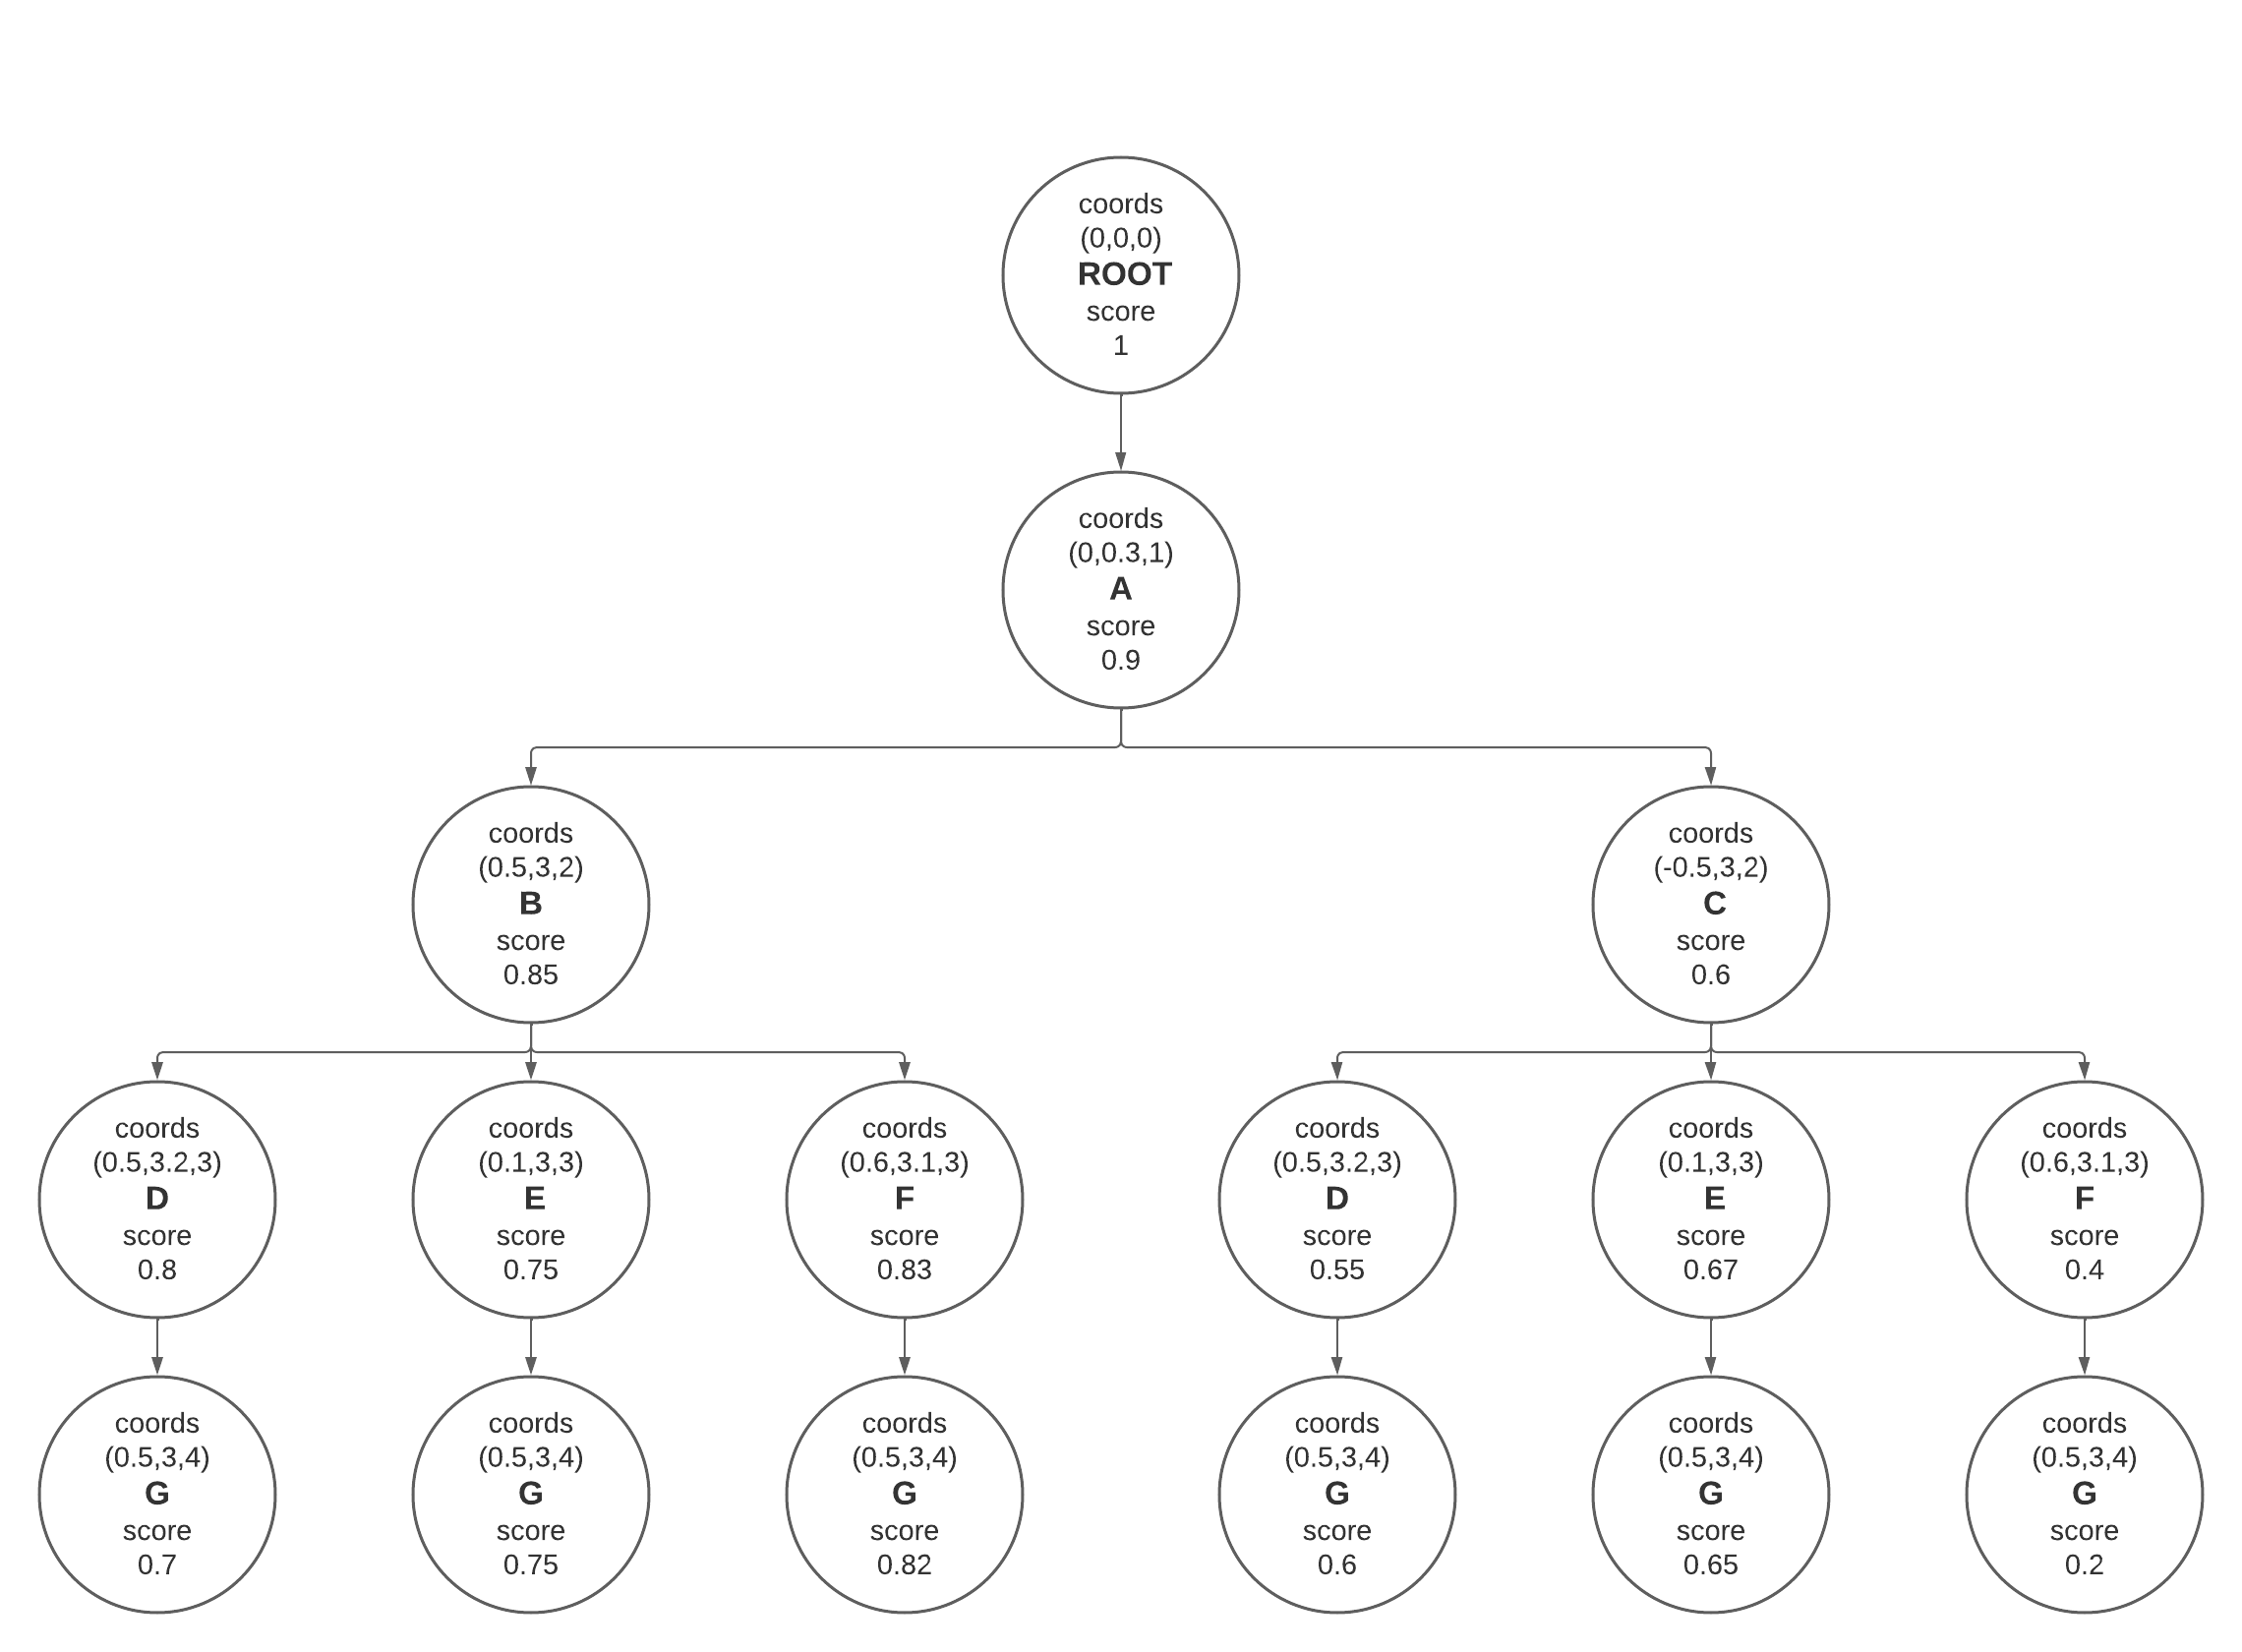
\includegraphics[width=13cm]{imaxes/Diagrama_arb.png}
    \caption{Ejemplo de un árbol de centroides}
    \label{fig:diagFlujoarb}
\end{figure}

Por lo que para evitar esto se guardan todos en una estructura de árbol que contiene las coordenadas del centroide y el ajuste a una linea con el resto de centroides, a cada nodo se le añaden los slices del siguiente slice. 
En la figura \ref{fig:diagFlujoarb} vemos como sería uno de estos árboles. Al tener el árbol lo que haremos será mirar los nodos hoja y mirar cuál es el que tiene mayor score, es decir, que mejor se ajuste a una línea y a partir de ese nodo iremos recorriendo la estructura de datos asta la raíz para obtener todos los centroides por los que pasa.

Para terminar mostraremos el código que realiza esta parte y lo comentaremos en relación al algoritmos explicado. Lo primero que hacemos para cada puntos es obtener la sección cilíndrica con el radio que definimos. A continuación para evitar detectar arbustos o maleza comprobamos si en ese cilindro hay un mínimo de puntos, este es un parámetro constante definido como constante.


Si tiene mas de el mínimo de puntos se procede a llamar a la función que divide ese cilindro en diferentes secciones y obtiene los centroides mediante el algoritmo que mencionamos antes. Una vez con los centroides volvemos a calcular el ajuste de los puntos y mediante un umbral decidimos si ese punto es realmente un árbol o no.

Ahora con la figura \ref{fig:ejemplotree} veremos un ejemplo de como seria el proceso para la obtención de los centroides. La figura \ref{fig:tree} es la nube de puntos de la sección tubular, en este ejemplo vemos claramente el tronco. A continuación en \ref{fig:tree_sliced} se ejemplifica como dividimos esa nube de puntos en 7 slices, para cada uno obtendremos los centroides y después de entre todos escogeremos los que mejor forme una linea \ref{fig:tree_sliced_centroids} y \ref{fig:tree_sliced_res}.




\begin{lstlisting}[language=Python, caption={Código para la busqueda de máximos }, label=lst:detectT]
def detect_trees(point_cloud, query_coords, radius_threshold):
    # create a list to save the locations of the trees that are tubular
    tubular_tree_locations = []
    no_tubular_tree_locations = []

    for query_coord in query_coords:

        distances = np.linalg.norm(point_cloud[:, :2] - query_coord[:2], axis=1)
        filtered_indices = np.where(distances <= radius_threshold)[0]
        filtered_points = point_cloud[filtered_indices]
        
        if len(filtered_points) < min_tree_samples:
            continue
        else:
            pcd = o3d.geometry.PointCloud()
            pcd.points = o3d.utility.Vector3dVector(filtered_points)
            
            centroids = slice_and_get_points_tree(filtered_points, slice_height)
            centroids = np.array(centroids)

            if len(centroids) > 4 and not np.isnan(centroids).any():

                r2 = calculate_r_squared(centroids)
                is_line = r2 > r_squared_threshold

                if is_line:
                    tubular_tree_locations.append(query_coord)
                else:
                    no_tubular_tree_locations.append(query_coord)
    return tubular_tree_locations
\end{lstlisting}

\begin{figure}[h]
  \begin{subfigure}{0.5\textwidth}
    \centering
    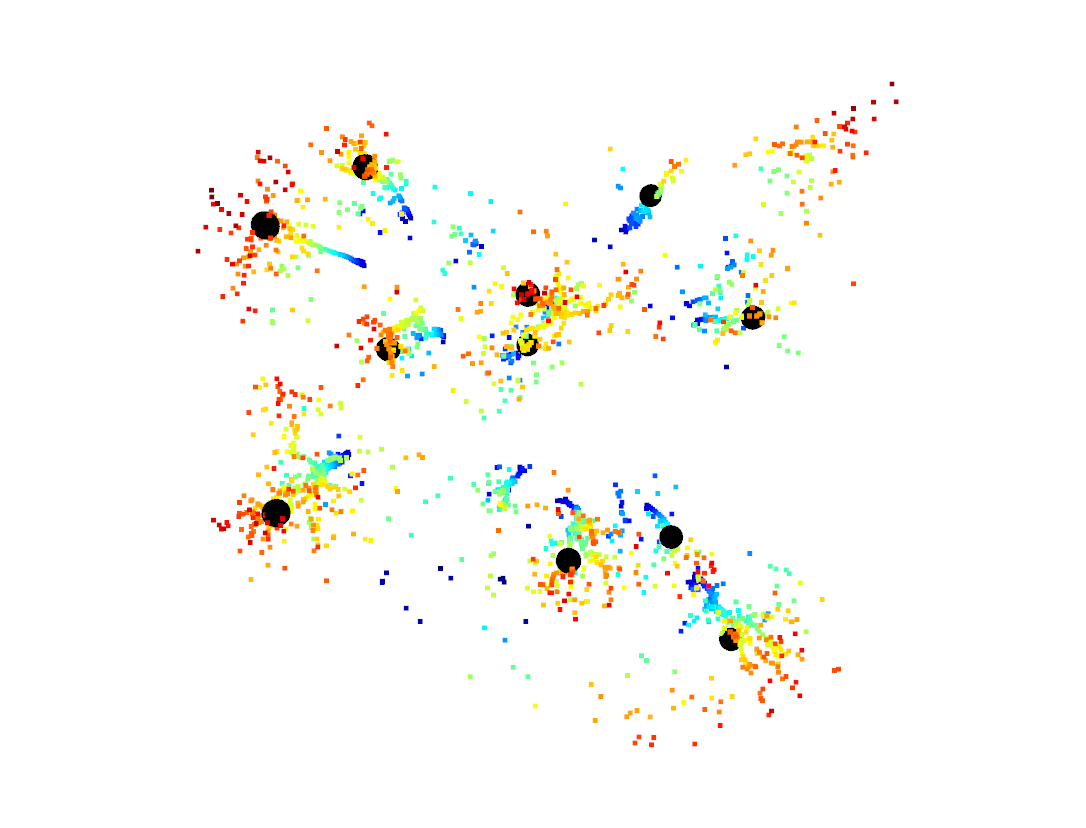
\includegraphics[width=0.8\linewidth]{imaxes/detecsup.png}
    \caption{Puntos detectamos árboles vista superior}
    \label{fig:last1}
  \end{subfigure}%
  \begin{subfigure}{0.5\textwidth}
    \centering
    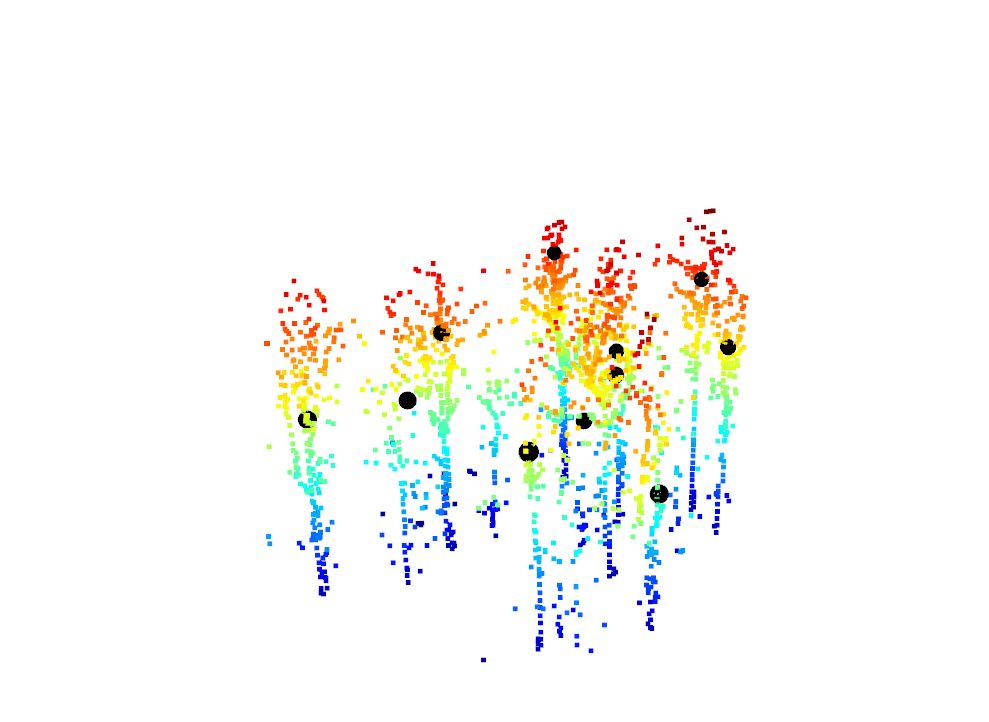
\includegraphics[width=0.8\linewidth]{imaxes/deteclat.png}
    \caption{Puntos detectamos árboles vista lateral}
    \label{fig:last}
  \end{subfigure}
  \caption{Ejemplo de puntos detectados como árboles, puntos negros son un árbol}
  \label{fig:algo2}
\end{figure}

\begin{figure}
\centering
\begin{subfigure}[t]{.5\textwidth}
  \centering
  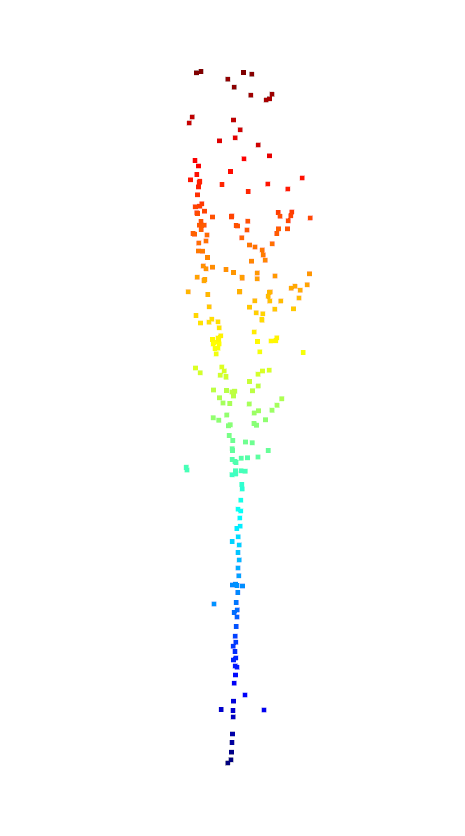
\includegraphics[height=5cm]{imaxes/tree.png}
  \caption{Nube de puntos del árbol}
  \label{fig:tree}
\end{subfigure}%
\begin{subfigure}[t]{.5\textwidth}
  \centering
  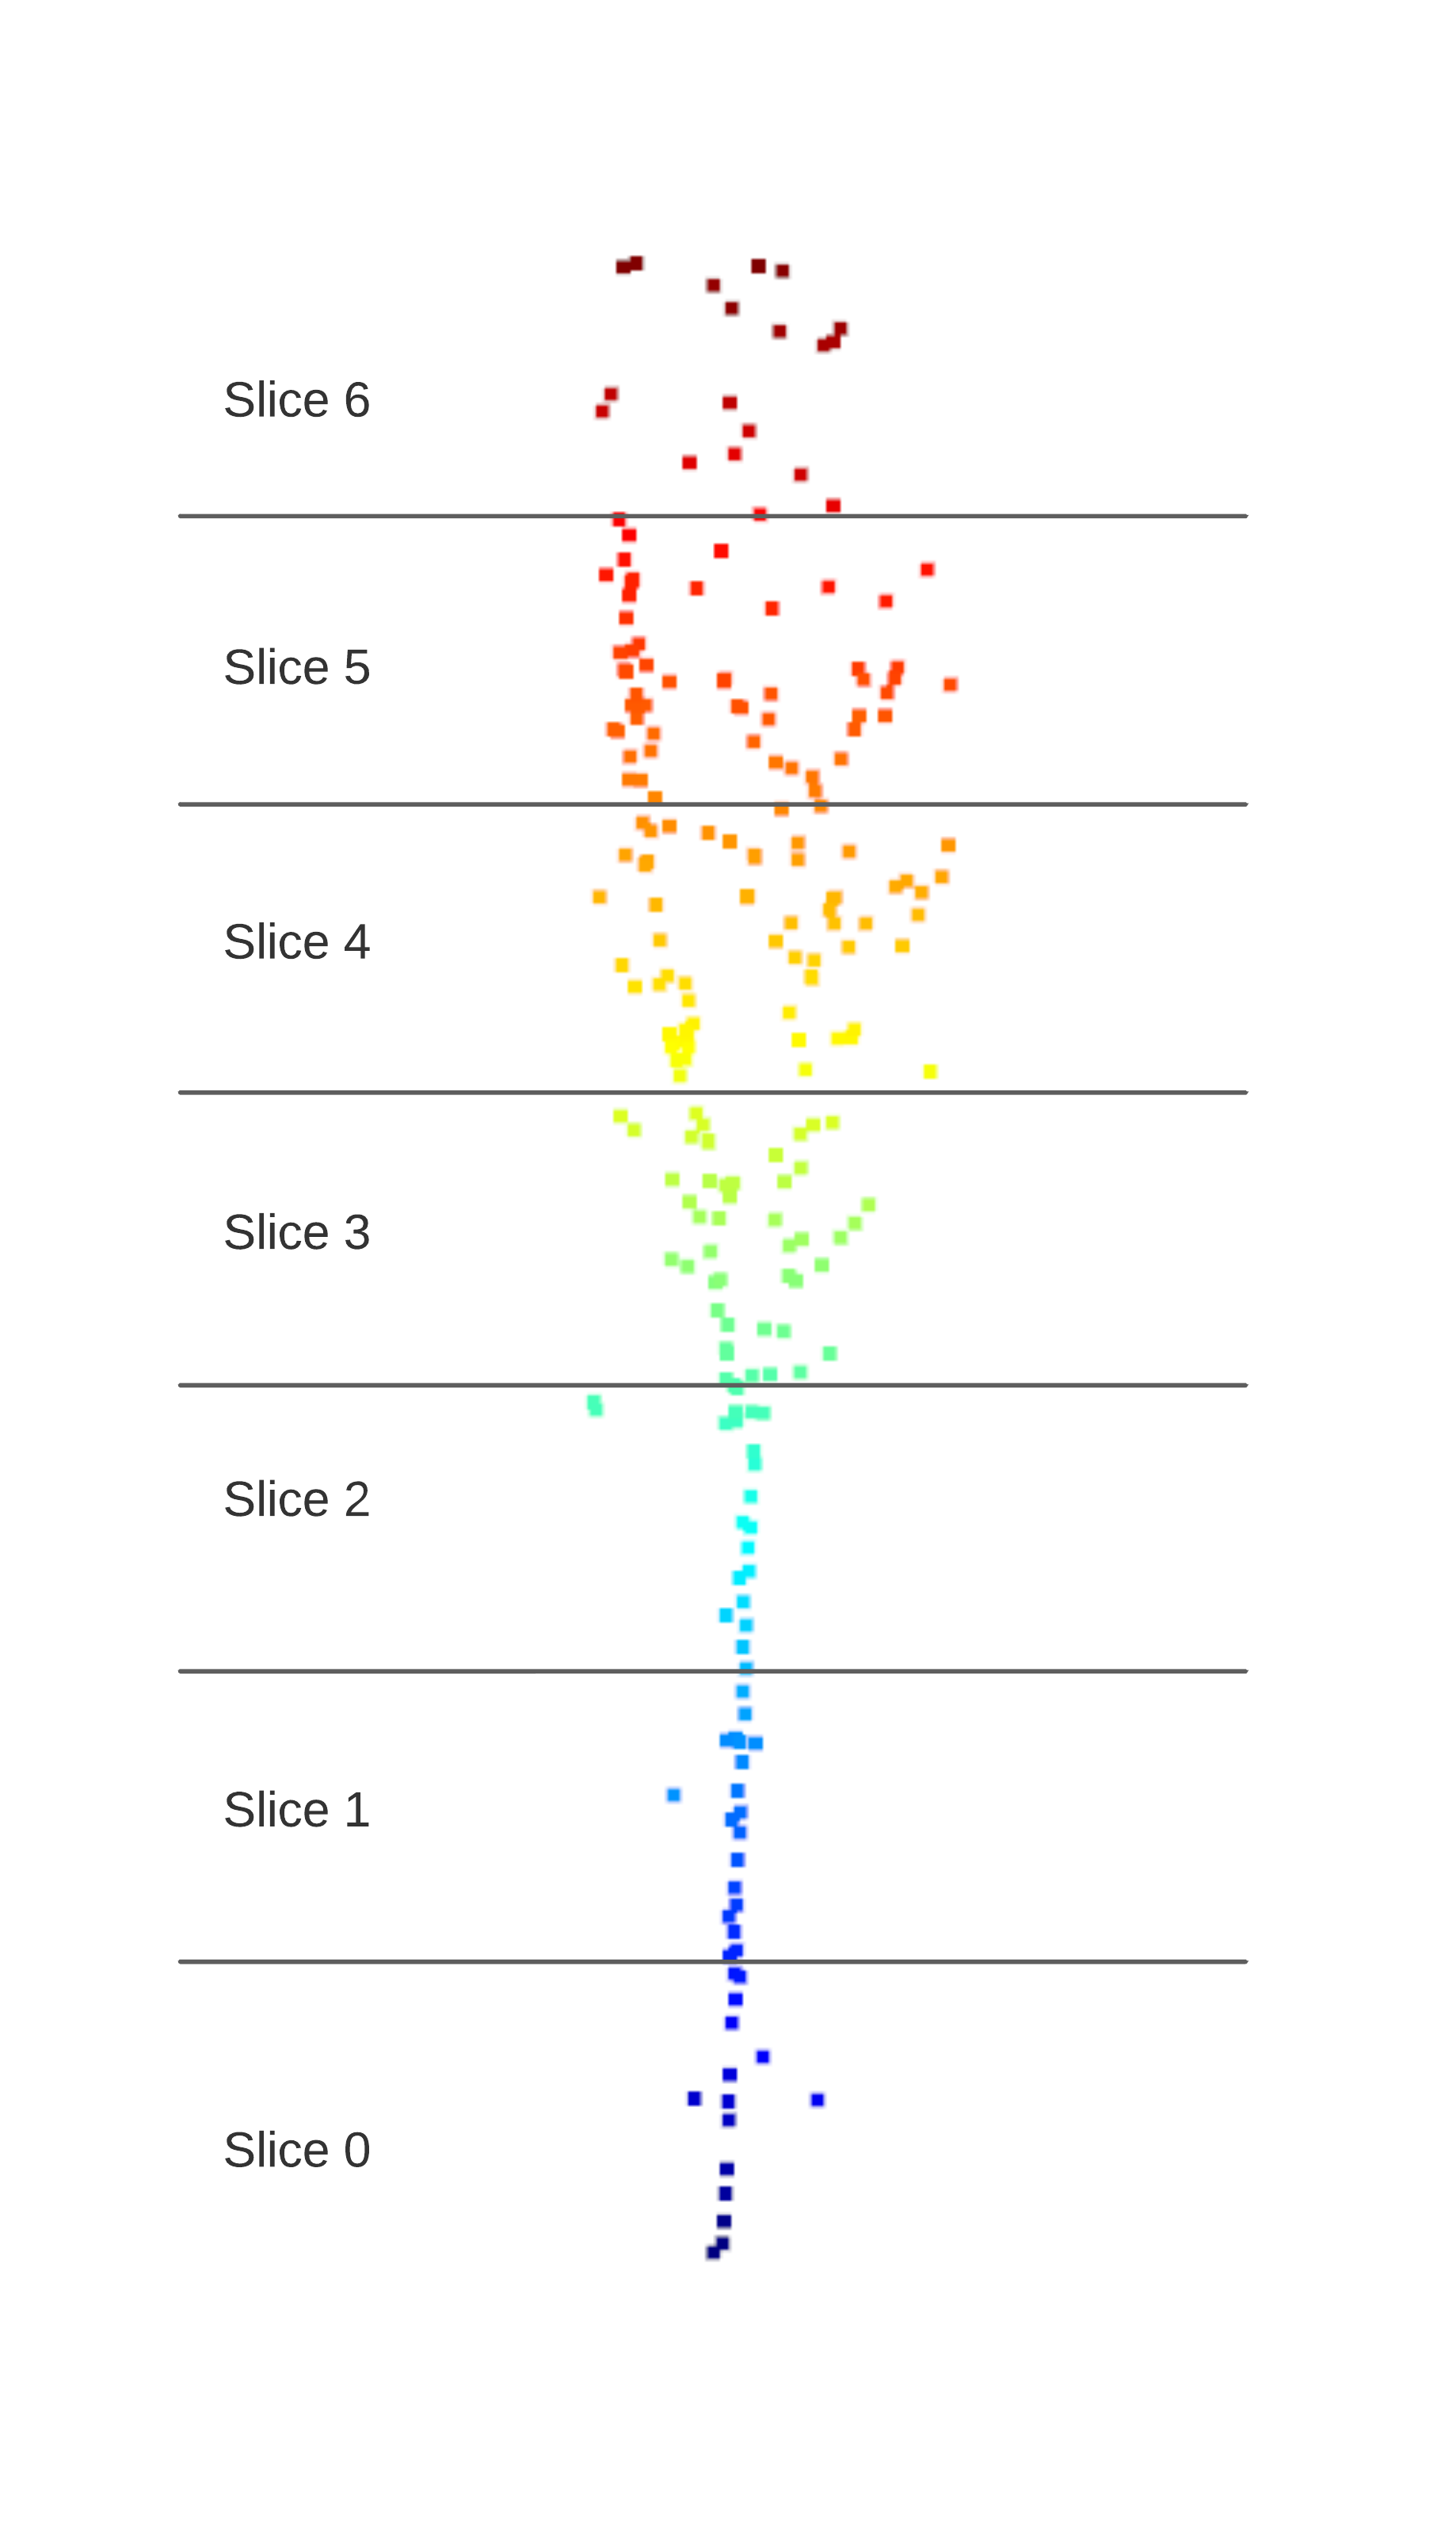
\includegraphics[height=5cm]{imaxes/tree_slices.png}
  \caption{Árbol dividida en 7 slices}
  \label{fig:tree_sliced}
\end{subfigure}

\begin{subfigure}[t]{.5\textwidth}
  \centering
  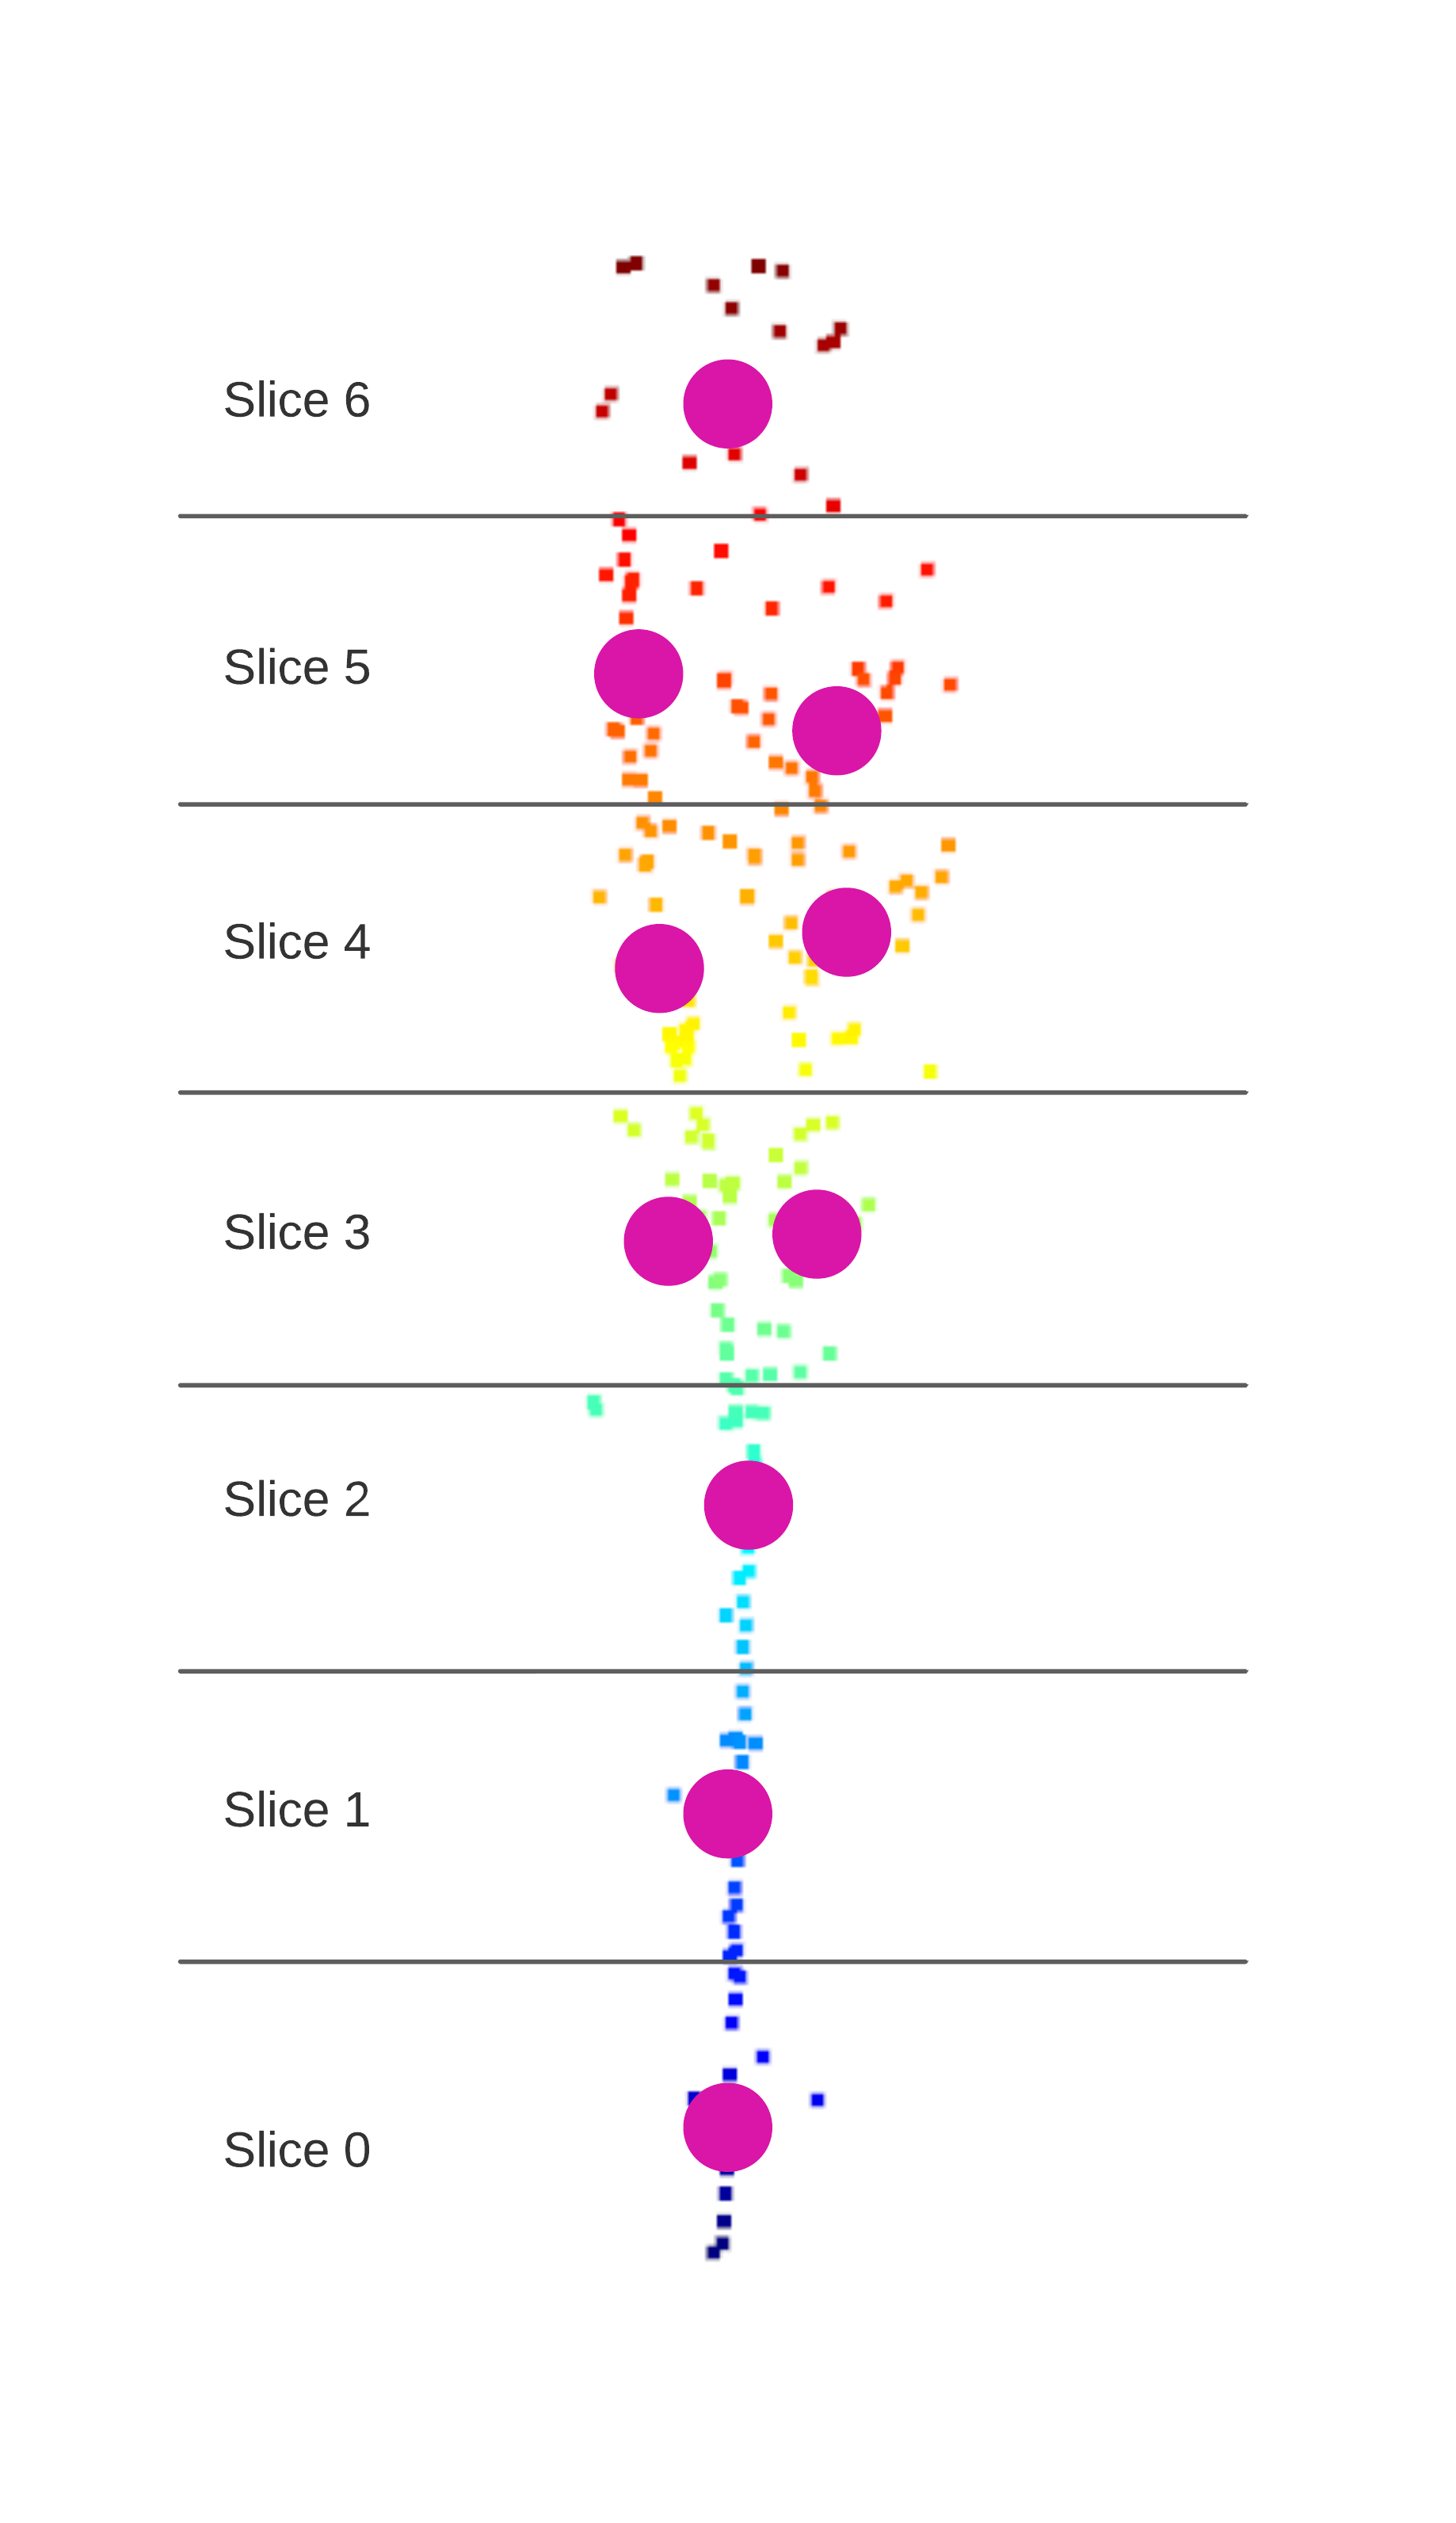
\includegraphics[height=5cm]{imaxes/tree_slices_centroids.png}
  \caption{Árbol con los centroides }
  \label{fig:tree_sliced_centroids}
\end{subfigure}%
\begin{subfigure}[t]{.5\textwidth}
  \centering
  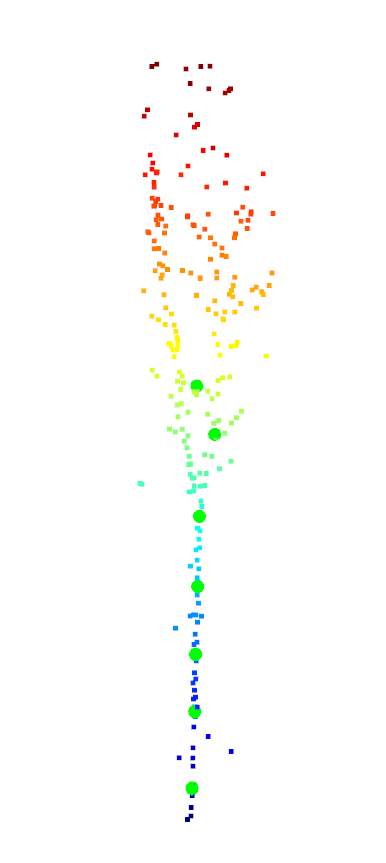
\includegraphics[height=5cm]{imaxes/tree_centroides.png}
  \caption{Árbol con centroides ajustados}
  \label{fig:tree_sliced_res}
\end{subfigure}

\caption{Ejemplo del proceso de obtención de los slices}
\label{fig:ejemplotree}
\end{figure}





\chapter{Resultados Experimentales}
\label{chap:Resultados}
\lettrine{E}{n} este capitulo expondremos los resultados obtenidos al ejecutar nuestro algoritmo en un entorno de pruebas. También explicaremos el entorno donde se desarrollaron y como se obtuvieron los datasets utilizados.

\section{Entorno de pruebas}
A continuación explicaremos como se obtuvieron los datasets donde se realizaron estas pruebas. 
Para la obtención del dataset se siguió un procedimiento que podemos ver en la figura \ref{fig:flugdataset} y que ahora explicaremos paso a paso.

\begin{figure}[h]
\centering
    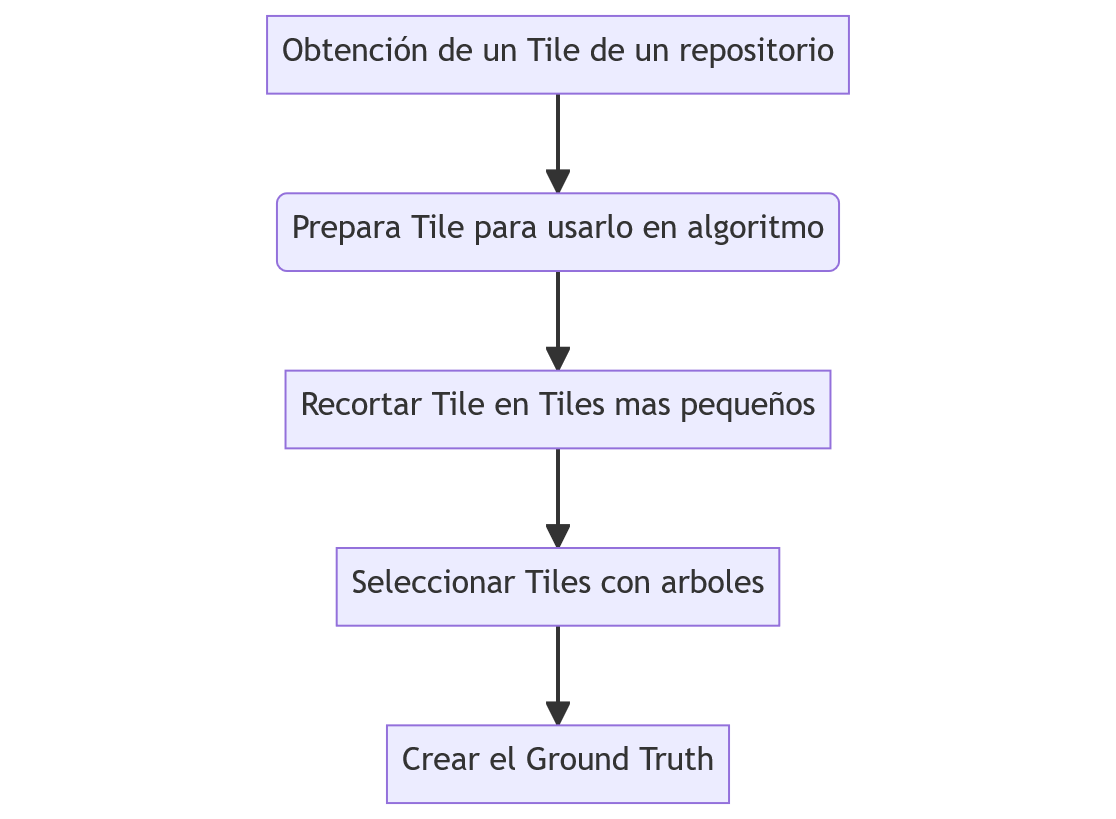
\includegraphics[width=10cm]{imaxes/mermaid-diagram-2023-09-02-195044.png}
    \caption{Diagrama de flujo para obtención del dataset}
    \label{fig:flugdataset}
\end{figure}

\subsection{Obtención del tile de un repositorio}
Primero tenemos que buscar un repositorio de datos LiDAR y seleccionar los tiles que usaremos. En nuestro caso optamos por usar el repositorio de Luxemburgo \cite{luxdata} como ya se comentó en la sección \ref{chap:investigPlan}.Se escogió este principalmente por su densidad de puntos que cumple con lo requerido y por ser libre para que cualquiera pueda usarlo.
Para nuestro entorno de prueba escogimos los tiles con identificador \textit{57000\_105000} y \textit{81500\_82500}.

\begin{figure}[h]
  \begin{subfigure}{0.5\textwidth}
    \centering
    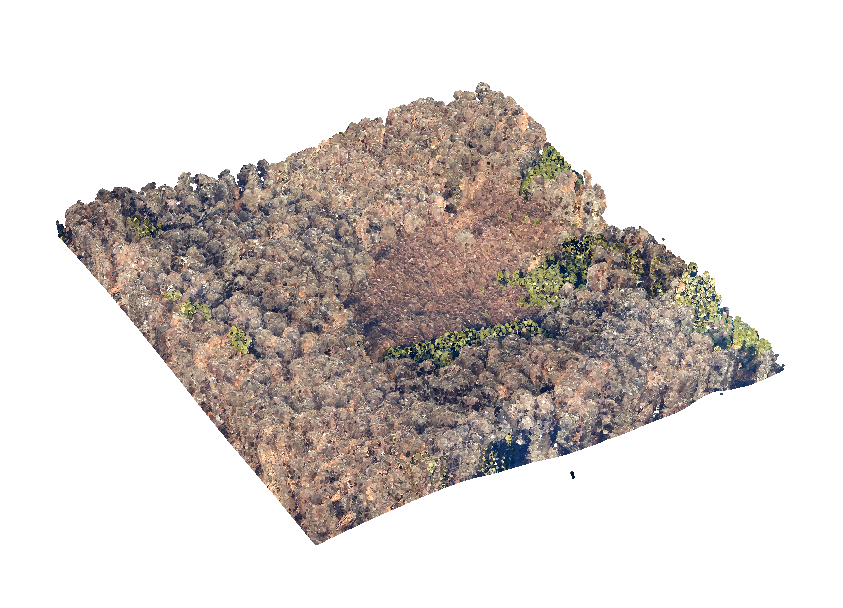
\includegraphics[scale=0.30]{imaxes/tile1.png}
    \caption{Tile 81500\_82500}
    \label{fig:tile1}
  \end{subfigure}
  \begin{subfigure}{0.5\textwidth}
    \centering
    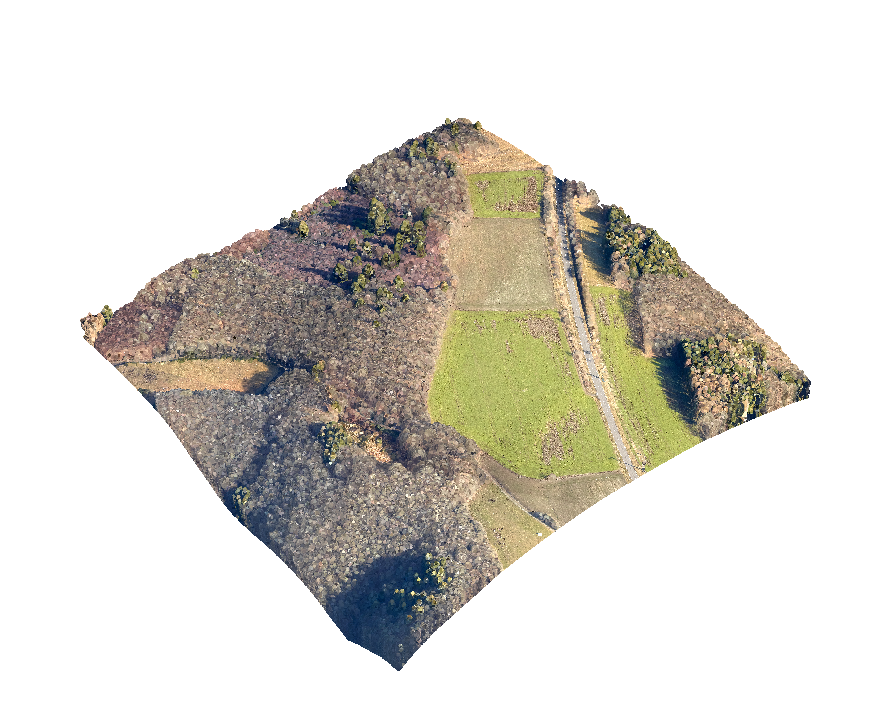
\includegraphics[scale=0.30]{imaxes/tile2.png}
    \caption{Tile 57000\_105000}
    \label{fig:tile2}
  \end{subfigure}
  \label{fig:restiles}
\end{figure}

\subsection{Preparación del Tile}
Como ya comentamos en el capitulo \ref{chap:Deteccion} necesitamos obtener un tile con las alturas normalizadas y con el ultimo retorno.A partir de eso necesitamos la versión con suelo para el mapa de alturas y otro sin el suelo para la detección. La explicación de como obtenerlos la encontramos en el capitulo \ref{chap:normalAlgo} , \ref{chap:LastAlgo} y \ref{chap:groundAlgo}.

\subsection{Recortar Tile en Tiles mas pequeños}
Para las prueba se decidió optar por recortar los tiles en trozos mas pequeños.Esto se hizo así por que el ground truth se hace de manera manual y por lo tanto generarlo para un tile tan grande sería prácticamente imposible y se cometerían muchos errores. Además también eliminas puntos que no son de interés como campos de cultivos o casas que lo único que hacen es ralentizar el proceso de prueba.

Para esta tarea se realizó un pequeño programa para recortar un tile grande en tiles mas pequeños cuadrados y todos del mismo tamaño. Después de esto escogeremos manualmente varios donde veamos que haya arboles y con diferentes tipos. En nuestro caso el dataset esta formado por 70 de estos tiles y con un total de 547 arboles de diferentes especies para que las métricas obtenidas sean reales.

\begin{figure}[h]
\centering
\begin{subfigure}[t]{.5\textwidth}
  \centering
  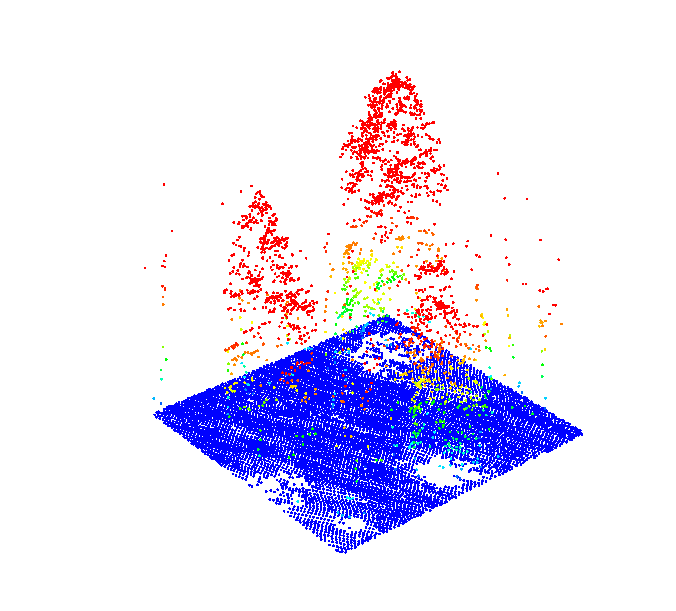
\includegraphics[height=5cm]{imaxes/subtile1.png}
\end{subfigure}%
\begin{subfigure}[t]{.5\textwidth}
  \centering
  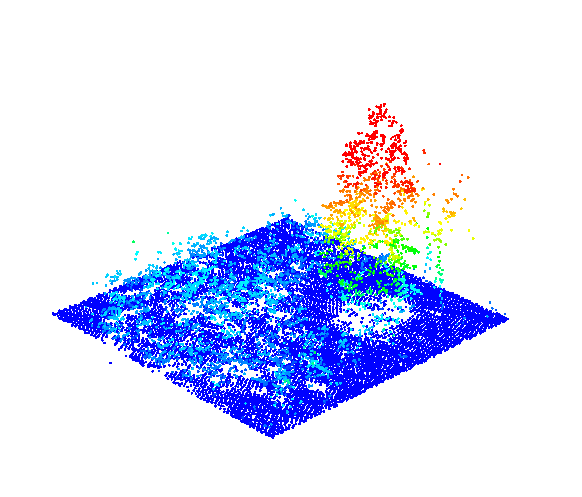
\includegraphics[height=5cm]{imaxes/subtile2.png}
\end{subfigure}

\begin{subfigure}[t]{.5\textwidth}
  \centering
  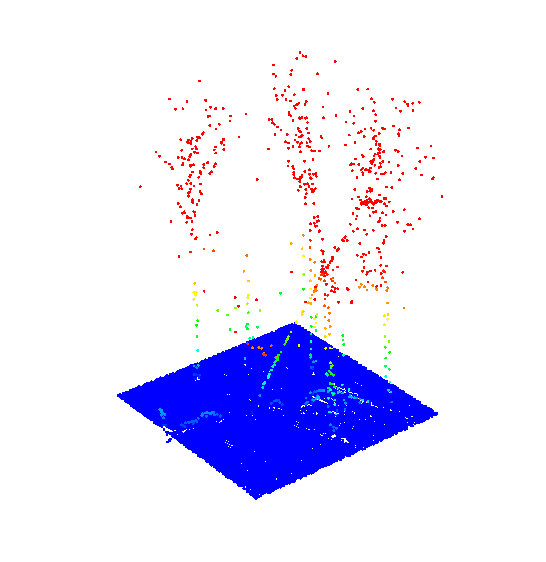
\includegraphics[height=5cm]{imaxes/subtile3.png}
\end{subfigure}%
\begin{subfigure}[t]{.5\textwidth}
  \centering
  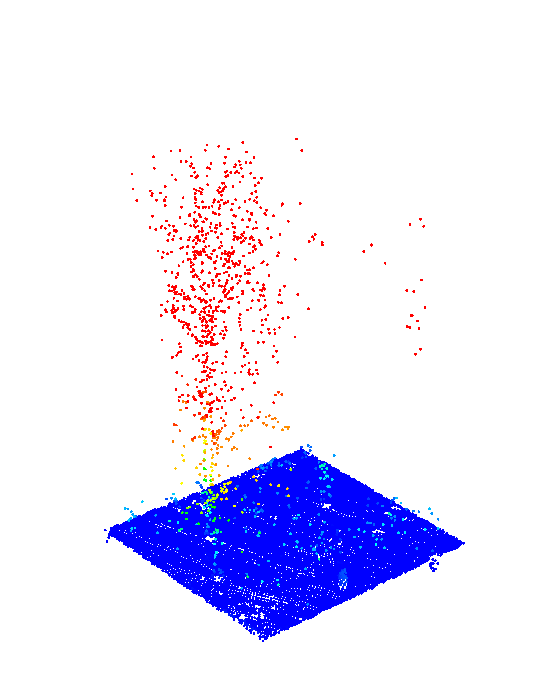
\includegraphics[height=5cm]{imaxes/subtile4.png}
\end{subfigure}

\caption{Ejemplo de tiles recortados}
\label{fig:ejemplotree}
\end{figure}

\subsection{Obtención del Ground Truth}
Una vez con los tiles preparados necesitamos un ground truth con la ubicación de los arboles.Para esta tarea también se desarrollo un pequeño programa para marcar estos mediante una interfaz gráfica como vemos en la figura \ref{fig:labelTile}.
En esta interfaz se nos muestra la nube de puntos y al hacer \textit{Shit} + \textit{Click Izquierdo} marcamos el punto donde esta el árbol, idealmente marcaremos donde se encuentre el tronco, en los casos donde no se pueda saber bien si es el tronco marcaremos la copa del árbol.

Una vez los seleccionemos todos al cerrar la interfaz se nos generará un archivo \textit{csv} con las coordenadas de los puntos. Este archivo es el que usaremos en un futuro para comprobar la precisión de la detección.

\section{Equipo de Pruebas}
Una vez con el dataset obtenido, comentaremos el equipo donde se realizaron estas pruebas. Para los test usamos una PC de sobremesa con las especificaciones que podemos ver en esta tabla 

\begin{table}[h]
\centering
\rowcolors{2}{white}{udcgray!25}
\begin{tabular}{c|c}
\rowcolor{udcpink!25}
\textbf{Especificación} & \textbf{Valor} \\\hline

CPU & Ryzen 5 1600 6c 12t 3.20 GHz\\
Memoria RAM & 16 gb 2666 mhz \\
GPU & Nvidia GTX 1060 6 gb \\
OS & Windows 10 Home 22H2 \\


\end{tabular}
\caption{Tabla con las especificaciones del equipo usado}
\label{tabcospes}
\end{table}


\begin{figure}[h]
\centering
    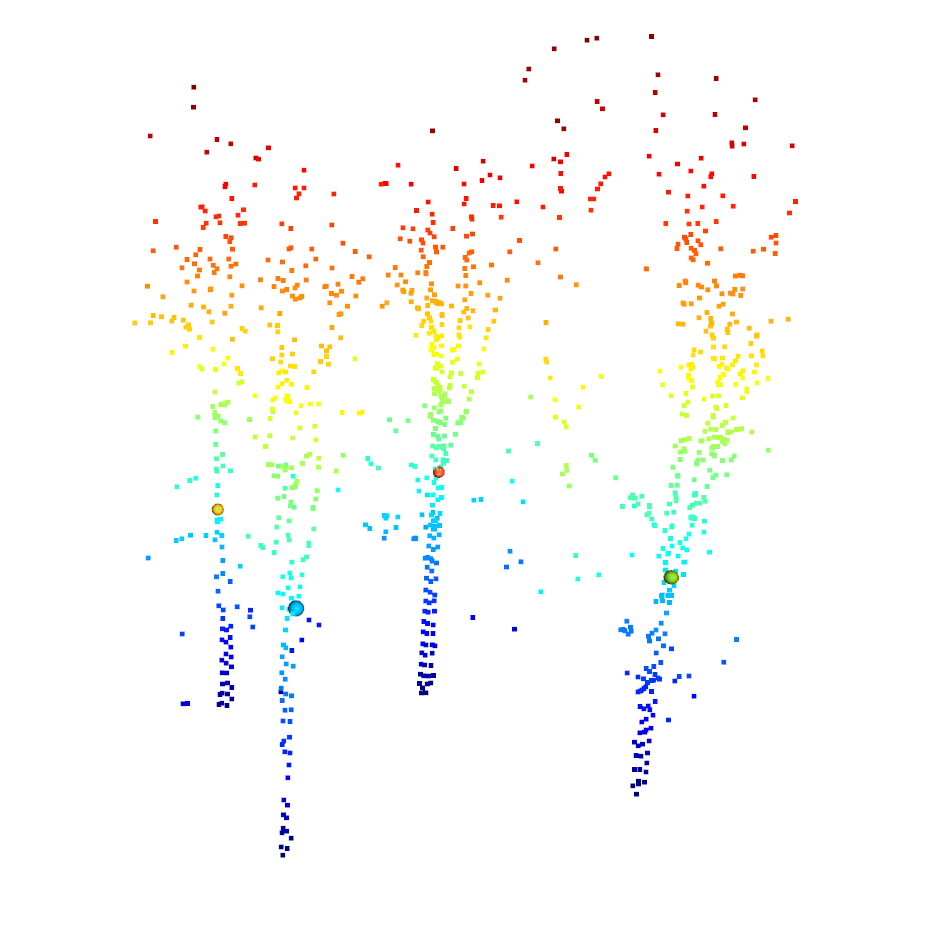
\includegraphics[width=7cm]{imaxes/marking.png}
    \caption{Programa para marcar los arboles}
    \label{fig:labelTile}
\end{figure}

\section{Parámetros de Prueba}

Antes de revisar los resultados de las pruebas, es esencial definir los parámetros utilizados en su realización. En primer lugar, estableceremos la resolución del mapa de alturas, que influye en la calidad y la resolución del mapa. Esta variable se establecerá en \textit{\textbf{0.005}}. A continuación, determinaremos el tamaño de la vecindad, en este caso, \textit{\textbf{80}}, y el umbral necesario para determinar si un valor es un máximo, que se fijará en \textit{\textbf{0.3}}.

En lo que respecta a la detección por estratos, estableceremos el número mínimo de puntos requeridos para considerar que un objeto es un árbol, que será \textit{\textbf{40}}. Además, definiremos el tamaño de los slices como \textit{\textbf{1}}, y el umbral necesario para determinar si el ajuste de la línea es suficientemente bueno, que será \textit{\textbf{0.1}}.

A continuación, presentaremos estos valores en una tabla \ref{tablavar} para una visualización más rápida.
\begin{table}[h]
\centering
\rowcolors{2}{white}{udcgray!25}
\begin{tabular}{c|c}
\rowcolor{udcpink!25}
\textbf{Especificación} & \textbf{Valor} \\\hline

Resolución del mapa de altura & 0.005 \\
Tamaño de vecindad & 80 \\
Umbral detección en máximos & 0.3 \\
Mínimo de puntos por estrato & 40 \\
Tamaño de "Slice" & 1 \\
Umbral Linealidad & 0.1 \\


\end{tabular}
\caption{Tabla con el valor de las constantes}
\label{tablavar}
\end{table}

\section{Resultados}
En esta sección comentaremos los resultados obtenidos y las métricas obtenidas tras los test en el conjunto de datos obtenido mediante el proceso anteriormente explicado.

Para poder entender lo que pasa en el sistema necesitamos una manera de cuantificar que tan bien esta funcionando, para esta cuantificación se usaron las métricas mas comunes en el campo de clasificación, la \textit{precisión}, la \textit{especialidad}, la \textit{exactitud} y la \textit{sensibilidad}. A mayores con estés valores obtendremos el \textit{F1 Score}

La obtención se explica en la imagen \ref{fig:confmatrix}, donde a la derecha vemos la matriz de confusión, esta es una herramienta utilizada para evaluar el rendimiento en los modelos de clasificación. Esta matriz organiza las predicciones hechas en un modelo de cuatro categorías:

\begin{itemize}
    \item \textbf{Verdaderos Positivos (True Positives, TP)} : Representa los casos en los que el modelo predice correctamente a que clase pertenece. En nuestro caso seria cuando detecta un árbol correctamente.
    \item \textbf{Verdaderos Negativos (True Negatives, TN)} :  Representa los casos en los que el modelo predice que no pertenece a una clase determinada y realmente ese objeto no pertenece a esa clase. Sería por ejemplo cuando detecta que un punto no es un árbol, en nuestro caso este valor no lo podemos obtener.
    \item \textbf{Falsos Postivos (False Positives, FP)} : Representa los casos en los que el modelo predijo incorrectamente a que pertenece a una clase determinada. En nuestro dominio sería cuando detecta que hay un árbol cuando realmente no lo hay.
    \item \textbf{Falsos Negativos (False Negatives, FN)} : Representa cuando el modelo predice que no pertenece a una clase cuando realmente si lo hace. Un ejemplo sería cuando el sistema detecta que no hay un árbol pero realmente si lo hay.
\end{itemize}

Una vez explicada la matriz de confusión explicaremos el significado de las métricas que hay en esta, usaremos todas menos la especialidad ya que no consideramos el caso no existir arboles.

\begin{itemize}
    \item \textbf{Precisión} : La precisión representa la proporción de perdiciones positivas correctas (TP) en relación a todas las predicciones positivas (TP + TF). Esta métrica es útil para identificar que la detección de los arboles sea precisa y confiable.

    \item \textbf{Exactitud} : La exactitud representa la proporción de perdiciones correctas (TP + TN) en relación al total de perdiciones  (TP + TN + FP + FN). Esta métrica nos indica que ta bien esta clasificando los árboles que realmente son árboles y los que no son realmente árboles. En casos donde el dataset no este balanceado, por ejemplo donde haya mas especies que puedan favorecer al algoritmo esta métrica no es suficiente. 

    \item \textbf{Exhaustividad} : La sensibilidad representa la proporción de predicciones correctas (TP) en relación a todos las perdiciones verdaderas reales (TP + FN). Esta métrica nos permite ver si nuestro sistema es capaz de detectar las mayoría de los árboles evitando los falsos negativos.

    \item \textbf{Especialidad} : La especificidad representa la proporción de predicciones correctas (TP) en relación a todos los casos verdaderamente negativos (TN + FP). Esta métrica nos permite evaluar la capacidad de evitar detecciones erróneas en nuestro sistema, como por ejemplo en el caso de detectar un arbusto como árbol.

    \item \textbf{F1 Score} : Esta métrica combina la precisión y Sensibilidad en una sola métrica. Es importante no solo ser capaces de detectar arboles sino también asegurar que la detección sea precisa.
    
    \[ F1 Score = \frac{2 \cdot \text{Precisión} \cdot \text{Exhaustividad}}{\text{Precisión} + \text{Exhaustividad}} \]

\end{itemize}

\begin{figure}[h]
\centering
    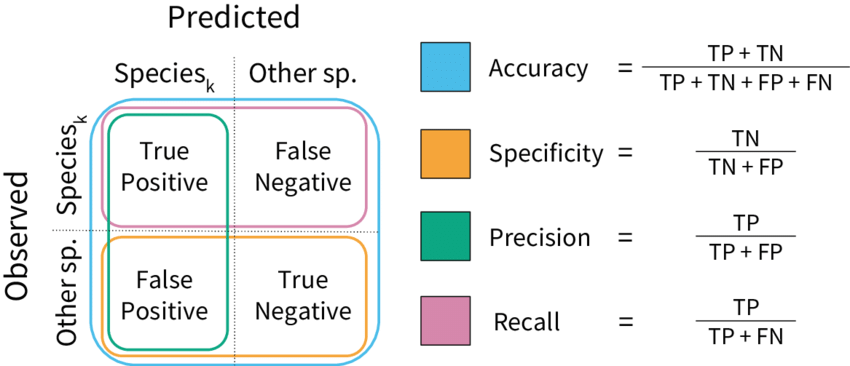
\includegraphics[width=13cm]{imaxes/Model-performance-metrics-Visual-representation-of-the-classification-model-metrics.png}
    \caption{Matriz de confusión con la manera de obtener las métricas usadas.\cite{imgConf}}
    \label{fig:confmatrix}
\end{figure}


Una vez con esto cabe remarcar que este sistema solo detecta si hay árboles, no detecta que no hay, por lo que las métricas como la Especialidad o Exactitud están acotadas para el caso exclusivo de existir arboles y no consideran el caso de no existir arboles.
Para comprobar si un árbol esta bien clasificado usamos las coordenadas del ground truth y comparamos si el punto que detectado esta cerca de un punto que es detectado como árbol, para esto definimos una distancia de margen de error.

Con esto aclarado procedemos a mostrar los resultados obtenidos en la tabla \ref{tablaconf} que contiene los valores de la matriz de confusión y en la tabla \ref{tablaMetr} que contiene las métricas.
\begin{table}[h]
\centering
\rowcolors{2}{white}{udcgray!25}
\begin{tabular}{c|c|c}
\rowcolor{udcpink!25}
\textbf{True positives} & \textbf{False Negatives} & \textbf{False Positives} \\\hline
486 & 300 & 61 \\
\end{tabular}
\caption{Valores de la matriz de confusión}
\label{tablaconf}
\end{table}

\begin{table}[h]
\centering
\rowcolors{2}{white}{udcgray!25}
\begin{tabular}{c|c|c|c}
\rowcolor{udcpink!25}
\textbf{Accuracy} & \textbf{Precision} & \textbf{Recall} & \textbf{F1 Score} \\\hline
59 \% & 68 \% & 89 \% & 70 \% \\
\end{tabular}
\caption{Métricas obtenidas con los valores de la matriz}
\label{tablaMetr}
\end{table}

Si miramos la precisión podemos ver como nuestro sistema tiene un valor de \textit{0.59} \% en un principio puede parecer baja pero no tiene que ser así. El dataset esta conformado por arboles de los dos principales tipos de bosques que existen en Luxemburgo, bosques caducifolios y bosques de coníferas \cite{luxfores}. Esto se hizo con el fin de tener un conjunto de datos fiel a la realidad del país del cual se tomaron los datos, el problema de esto es que en los bosques de coníferas como las piceas estas tiene mucho mas ramaje mucho mas denso y con las densidades que trabajamos perdemos el tronco al obtener el ultimo retorno, en el caso de bosques caducifolios habitados por robles, castaños y hayas si la densidad de puntos es buena nos permite ver claramente el tronco y nuestro algoritmo obtiene una mayor precisión. 

\begin{figure}
\centering
  \begin{subfigure}{0.5\textwidth}
    \centering
    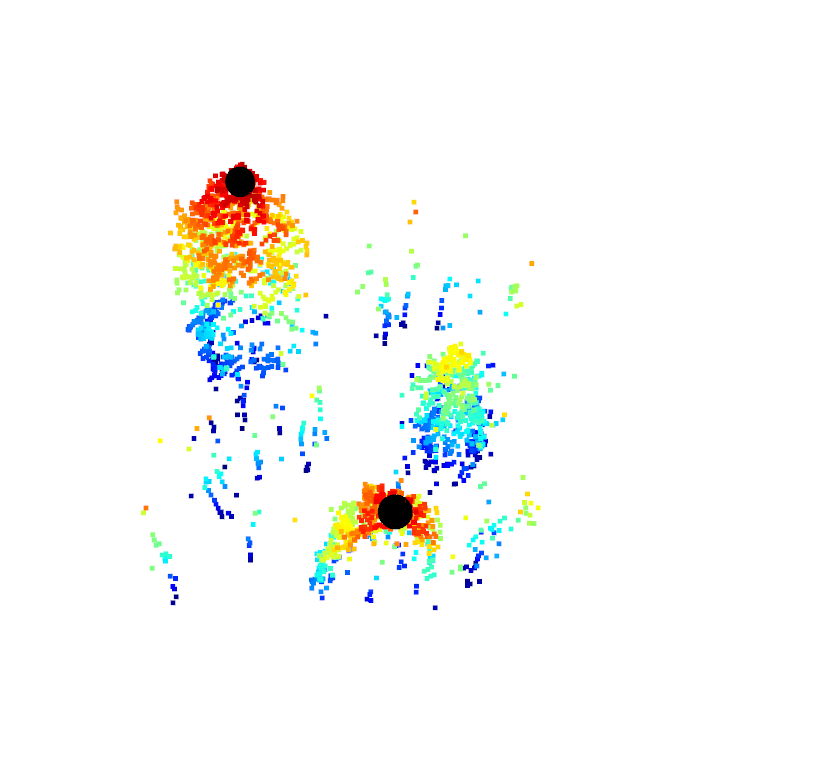
\includegraphics[width=0.9\linewidth]{imaxes/resdet1.png}
    \caption{Árboles detectados vista superior}
  \end{subfigure}%
  
  \begin{subfigure}{0.5\textwidth}
    \centering
    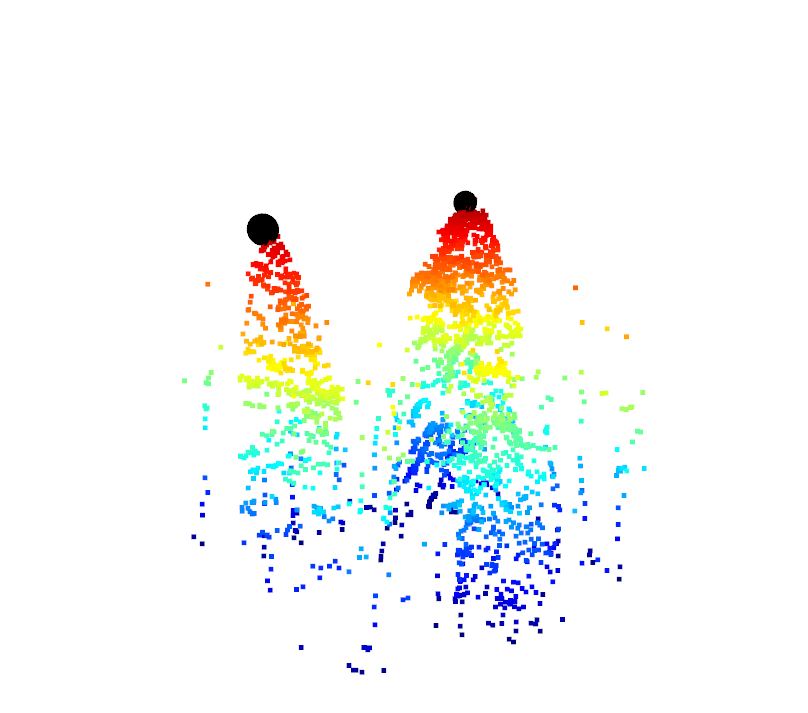
\includegraphics[width=0.9\linewidth]{imaxes/resdet1lat.png}
    \caption{Árboles detectados vista lateral}

  \end{subfigure}%
  
  \begin{subfigure}{0.5\textwidth}
    \centering
    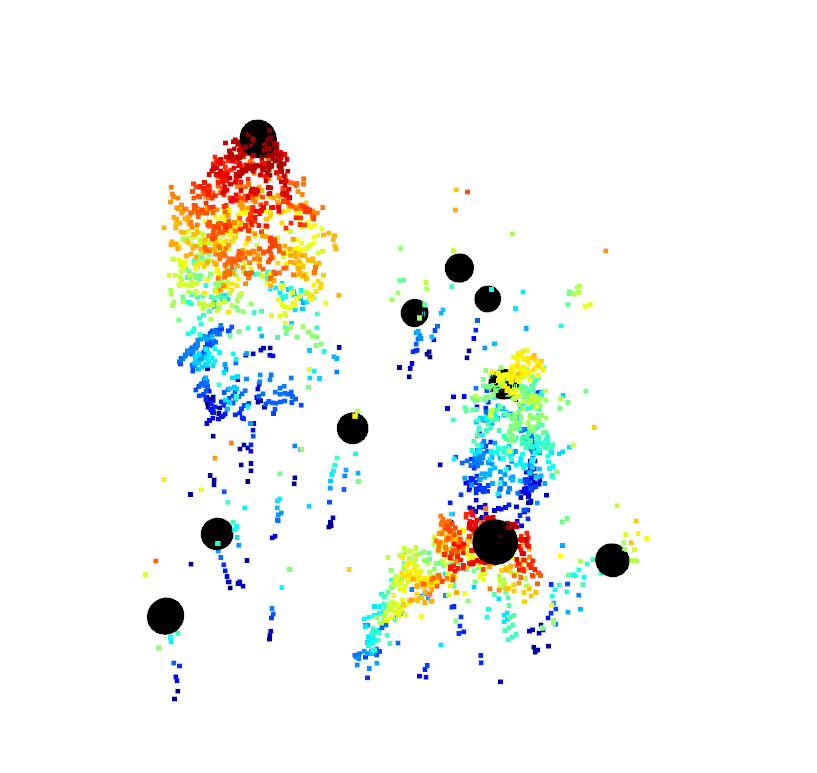
\includegraphics[width=0.9\linewidth]{imaxes/groundT.png}
    \caption{Ground Truth}
  \end{subfigure}
    
  \caption{Ejemplo de Detección en Coníferas}
  \label{detecAna}
\end{figure}

\begin{figure}
  \begin{subfigure}{0.5\textwidth}
    \centering
    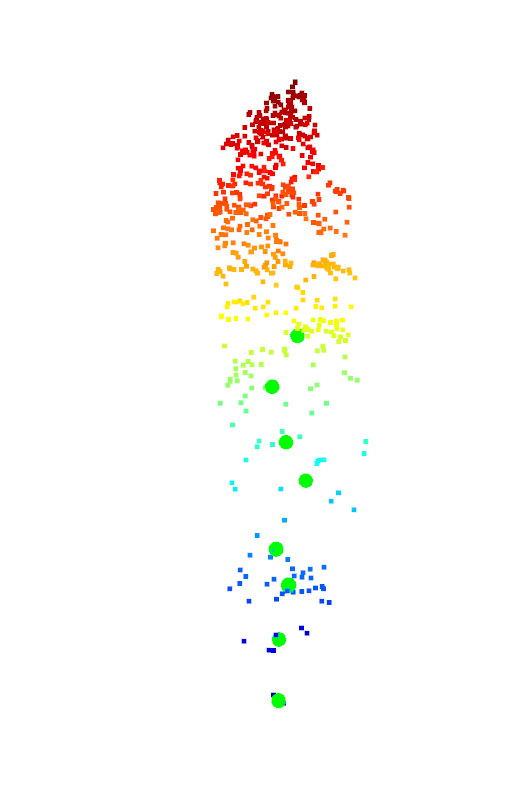
\includegraphics[width=0.8\linewidth]{imaxes/centroides1.png}
  \end{subfigure}%
  \begin{subfigure}{0.5\textwidth}
    \centering
    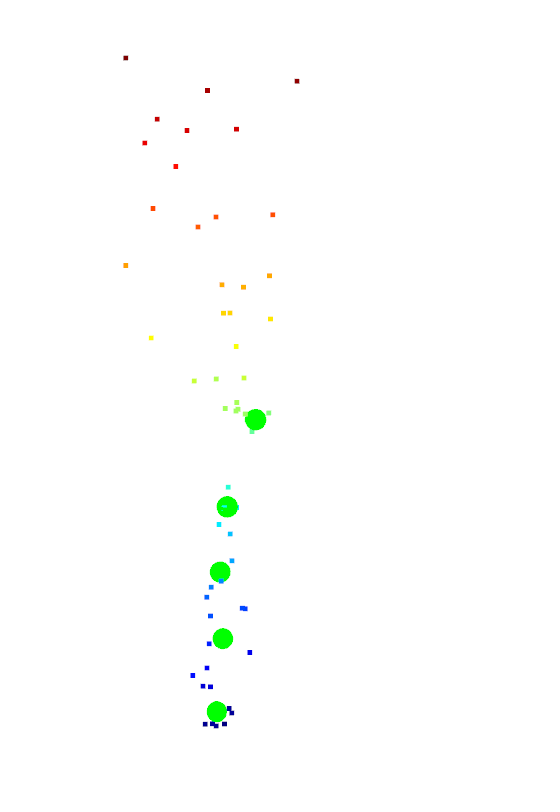
\includegraphics[width=0.8\linewidth]{imaxes/centroide2.png}
  \end{subfigure}
 \caption{Ejemplo de los centroides que son detectados como árboles}
  \label{fig:centroidesAna}
\end{figure}

\begin{figure}
  \begin{subfigure}{0.5\textwidth}
    \centering
    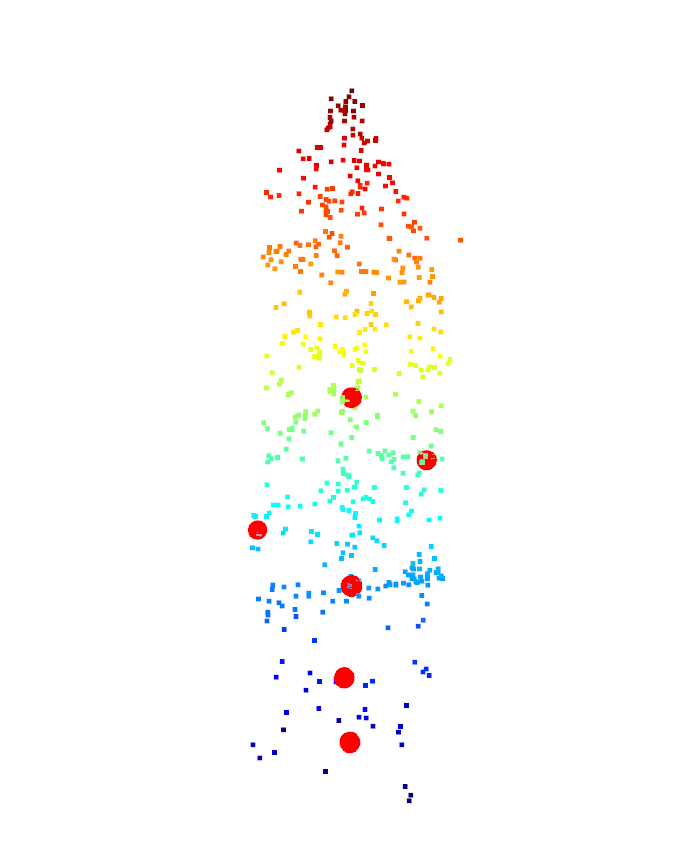
\includegraphics[width=0.8\linewidth]{imaxes/resdetec1fallido.png}
  \end{subfigure}
  \begin{subfigure}{0.5\textwidth}
    \centering
    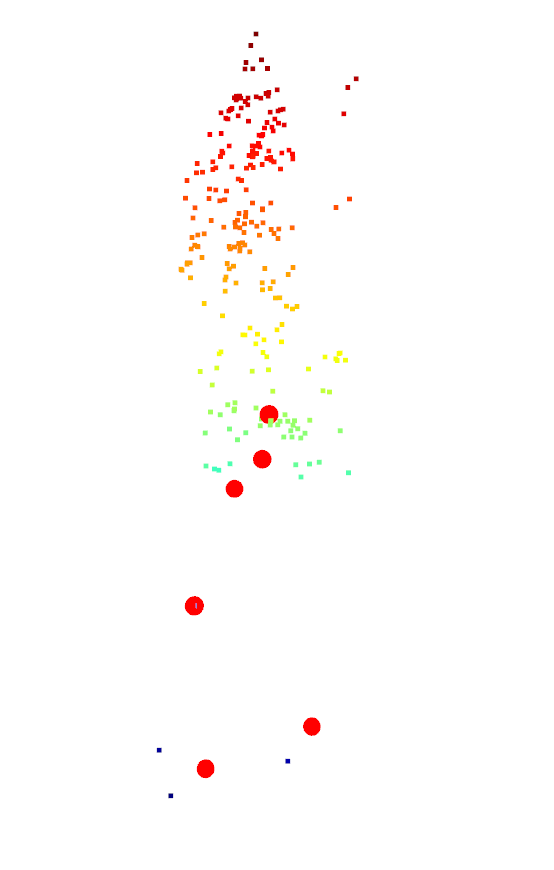
\includegraphics[width=0.8\linewidth]{imaxes/resdetec2fallido.png}
  \end{subfigure}
 \caption{Ejemplo de los centroides que no son detectados como árboles}
  \label{fig:centroidesAnaF}
\end{figure}


Si observamos el Recall podemos ver como nuestro sistema realmente detecta muchos arboles pero al mismo tiempo muchos son incorrectos, esto puede ser dado por los parámetros utilizados, aquí también influye el tipo de árbol, por lo general en los caducifolios las copas son mas extensas por lo que el tamaño de vecindad es mayor por lo que si el valor fuera demasiado bajo podría detectar varios arboles donde solo existe uno. Por la contra en el caso de coníferas as copas suelen ser mas pequeñas y en un mismo espacio hay mas por lo que el valor de vecindad alto podría dar a que solo obtuviéramos un árbol donde existen varios. Por esto mismo para tener un resultado lo mas realista posible se busco un valor intermedio que no beneficiara en exceso a ninguno de los dos.

En la figura \ref{detecAna} podemos ver un ejemplo de un tile donde las coníferas están bastante definidas pero los pequeños arboles como tiene una densidad e puntos muy baja el algoritmo los detecta como si fueran maleza. Además de esto en las figuras \ref{fig:centroidesAna} y \ref{fig:centroidesAnaF} podemos ver ejemplos de arboles donde los centroides forma una linea bastante definida y ese punto se clasifica como árbol y el caso contrario donde vemos que no tienen forma linea por lo tanto se rechaza.



\begin{figure}
  \begin{subfigure}{0.5\textwidth}
    \centering
    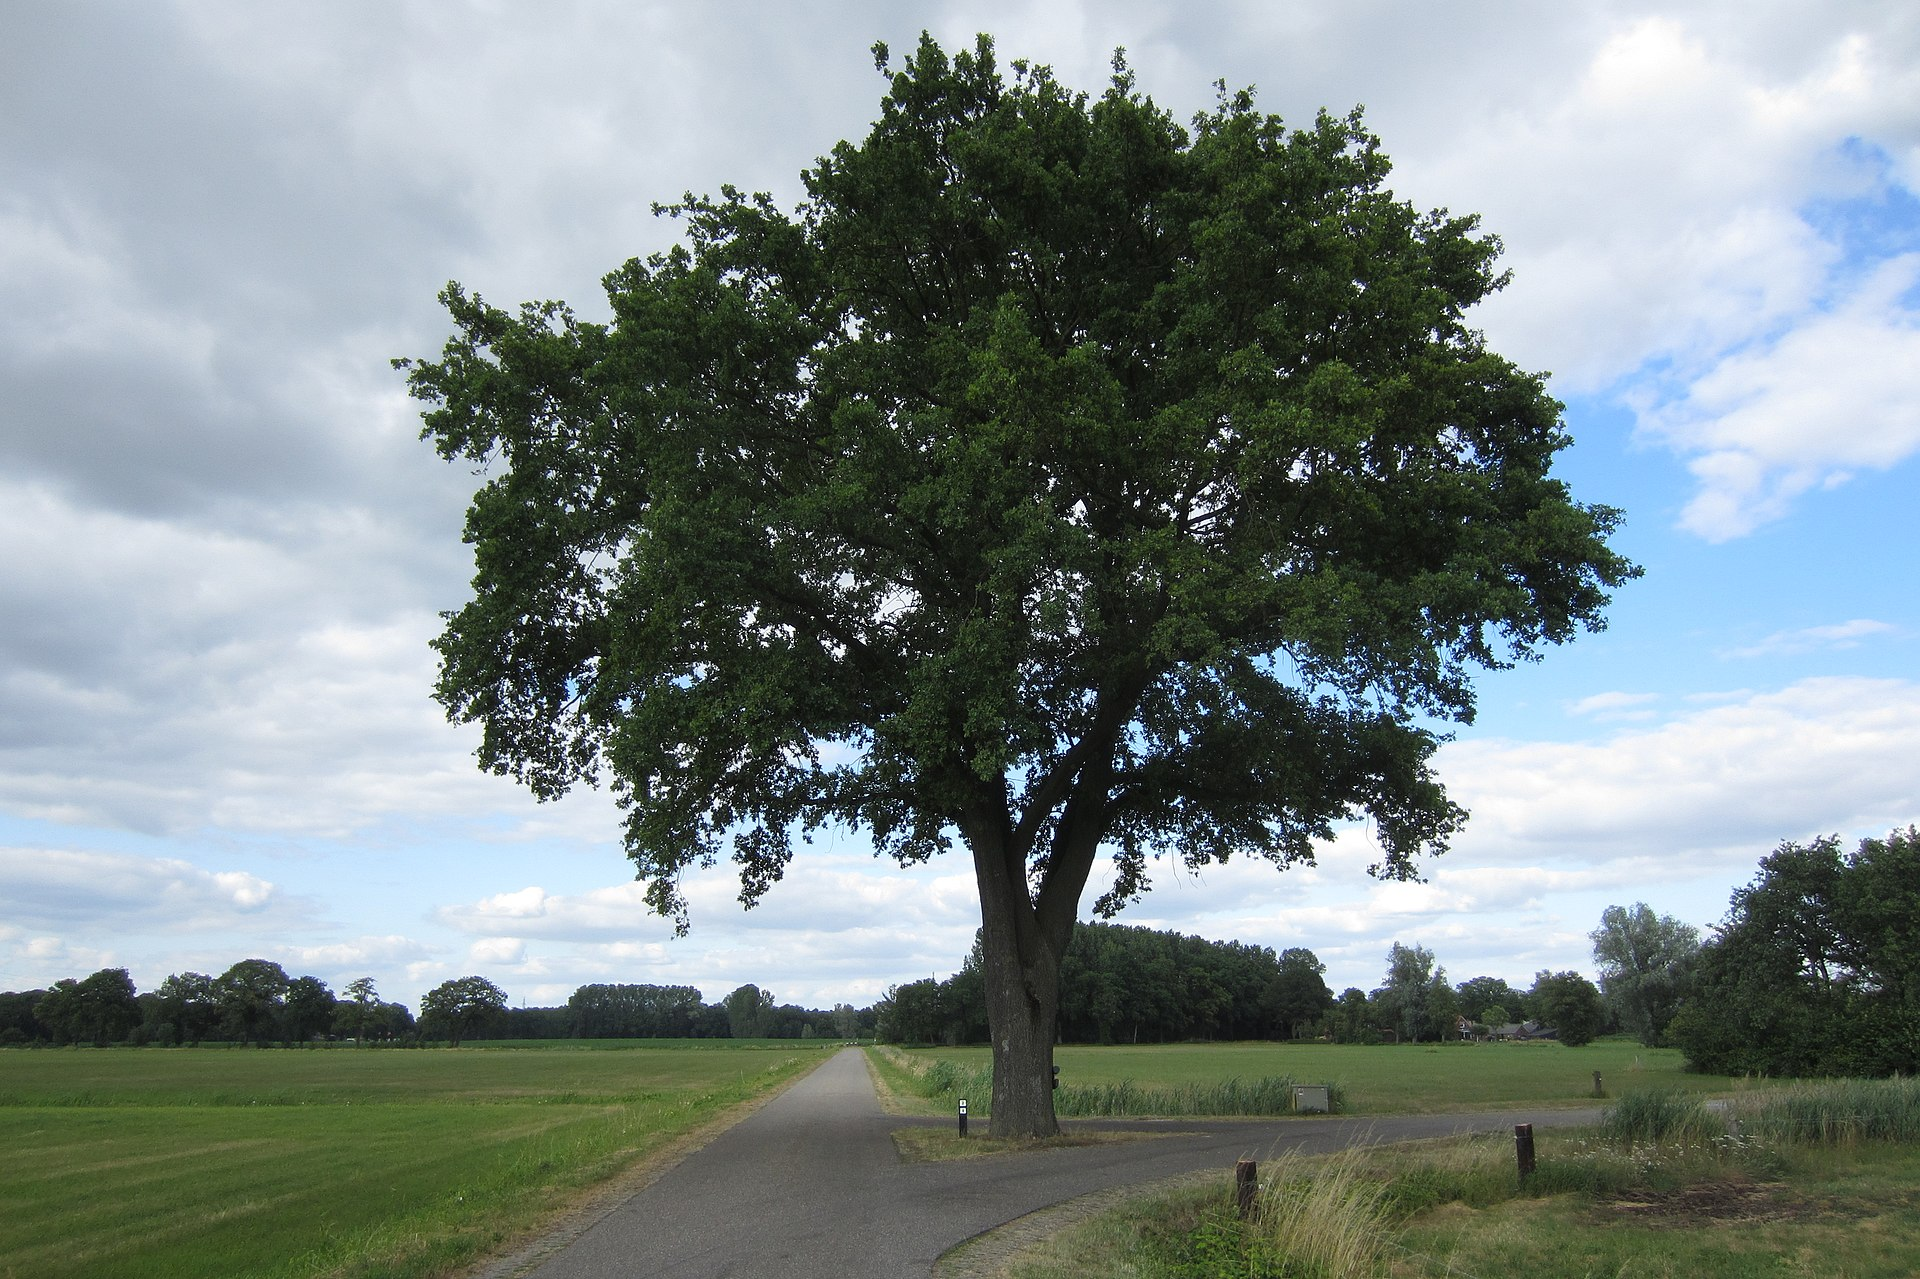
\includegraphics[width=0.8\linewidth]{imaxes/2019-07-03_Eik_in_Kerspel_Goor.jpg}
    \caption{Imagen de un roble}
  \end{subfigure}%
  \begin{subfigure}{0.5\textwidth}
    \centering
    \includegraphics[width=0.8\linewidth,height=0.9\linewidth]{imaxes/picea.jpg}
    \caption{Imagen de una picea}
  \end{subfigure}
\end{figure}

Para corroborar esto se escogieron 29 de los 70 tiles anteriores donde predominan los caducifolios y donde las nube de puntos tiene una buena densidad. Esta vez los parámetros los ajustamos para este tipo de bosque y nos quedaron como vemos en la tabla \ref{tablavar2}

\begin{table}[h]
\centering
\rowcolors{2}{white}{udcgray!25}
\begin{tabular}{c|c}
\rowcolor{udcpink!25}
\textbf{Especificación} & \textbf{Valor} \\\hline


Resolución del mapa de altura & 0.005 \\
Tamaño de vecindad & 140 \\
Umbral detección en máximos & 0.3 \\
Mínimo de puntos por estrato & 40 \\
Tamaño de slice & 1 \\
Umbral Linealidad & 0.1 \\

\end{tabular}
\caption{Tabla con el valor de las constantes para el test en caducifolios}
\label{tablavar2}
\end{table}

Tras ejecutar el mismo algoritmo en este dataset obtenemos los resultados que podemos ver en la tabla \ref{tablaconf2} y \ref{tablaMetr2} que son totalmente diferentes a los vistos previamente.

\begin{table}[!h]
\centering
\rowcolors{2}{white}{udcgray!25}
\begin{tabular}{c|c|c}
\rowcolor{udcpink!25}
\textbf{True positives} & \textbf{False Negatives} & \textbf{False Positives} \\\hline
139 & 15 & 46 \\
\end{tabular}
\caption{Valores de la matriz de confusión en el nuevo dataset}
\label{tablaconf2}
\end{table}
\begin{table}[!h]
\centering
\rowcolors{2}{white}{udcgray!25}
\begin{tabular}{c|c|c|c}
\rowcolor{udcpink!25}
\textbf{Accuracy} & \textbf{Precision} & \textbf{Recall} & \textbf{F1 Score} \\\hline
72 \% & 82 \% & 90 \% & 83 \% \\
\end{tabular}
\caption{Métricas obtenidas con los valores de la matriz en el nuevo dataset}
\label{tablaMetr2}
\end{table}

Aquí vemos como ahora no tenemos una precisión mayor y nuestro sistema es mas exacto, la precisión tiene un porcentaje de mejora del 20 \% lo que es bastante, el Recall se mantiene por la cantidad de árboles que detectamos sigue siendo alta. En general podemos ver mejores resultados este tipo de entorno, pero aun así esto podría estar condicionado por la densidad de puntos, para un análisis mas exhaustivo seria necesario tener un conjunto de datos de pruebas con varias especies y con densidades de puntos mas altas que estas, estas se podrían obtener mediante escaneos terrestres o con drones con un sensor equipado.

Por último comentar los tiempos de ejecución, la ejecución del entorno de prueba tomo 59 segundos lo que es un valor bastante alto si lo relacionamos con lo que realmente tardaríamos en procesar 2 tiles enteros.
Cada Tile lo dividimos en 320 subtiles aproximadamente, es decir los dos tiles serian 740 subtiles. Si hacemos una regla de tres con los 59 segundos que tarda en ejecutar 70 tiles tendríamos que tardaría 10 minutos en procesar los 2 tiles. En el capitulo \ref{chap:conclusions} comentaremos opciones para mejorar este resultado.


\begin{figure}[h]
\centering
  \begin{subfigure}{0.5\textwidth}
    \centering
    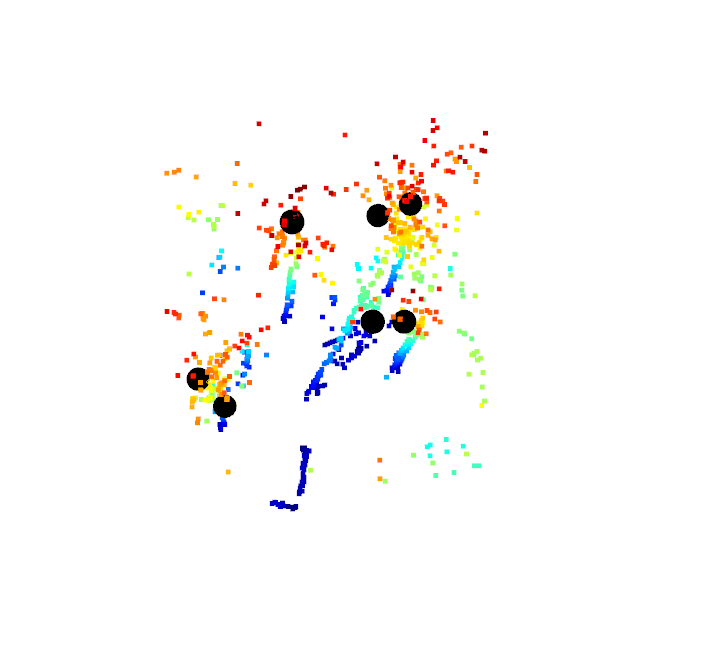
\includegraphics[width=0.9\linewidth]{imaxes/detectcad1.png}
    \caption{Árboles detectados vista superior}
    \label{fig:last1}
  \end{subfigure}%
  
  \begin{subfigure}{0.45\textwidth}
    \centering
    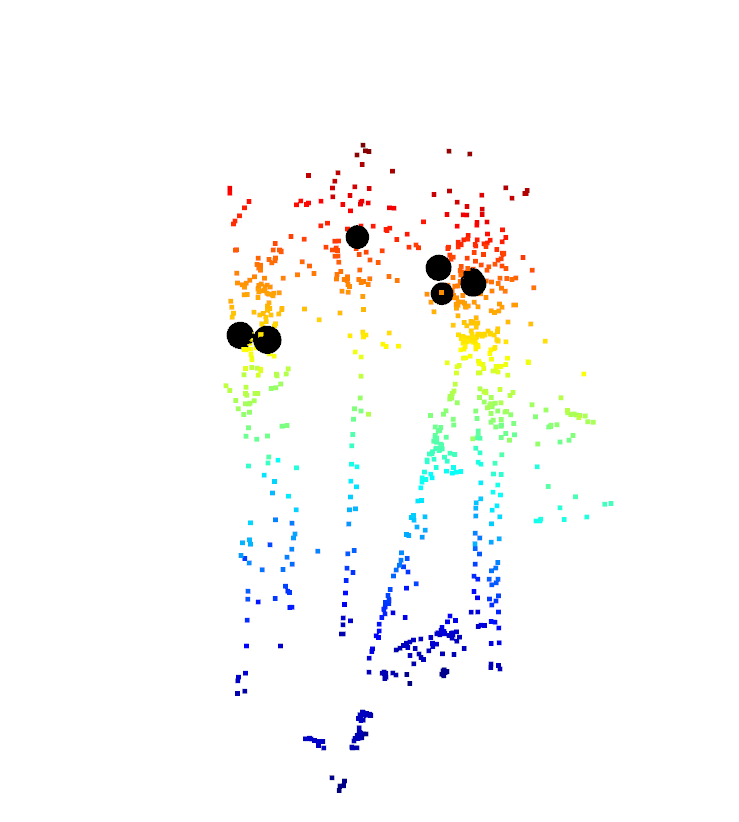
\includegraphics[width=0.9\linewidth]{imaxes/detecad1lat.png}
    \caption{Árboles detectados vista lateral}
    \label{fig:last2}
  \end{subfigure}%
  
  \begin{subfigure}{0.45\textwidth}
    \centering
    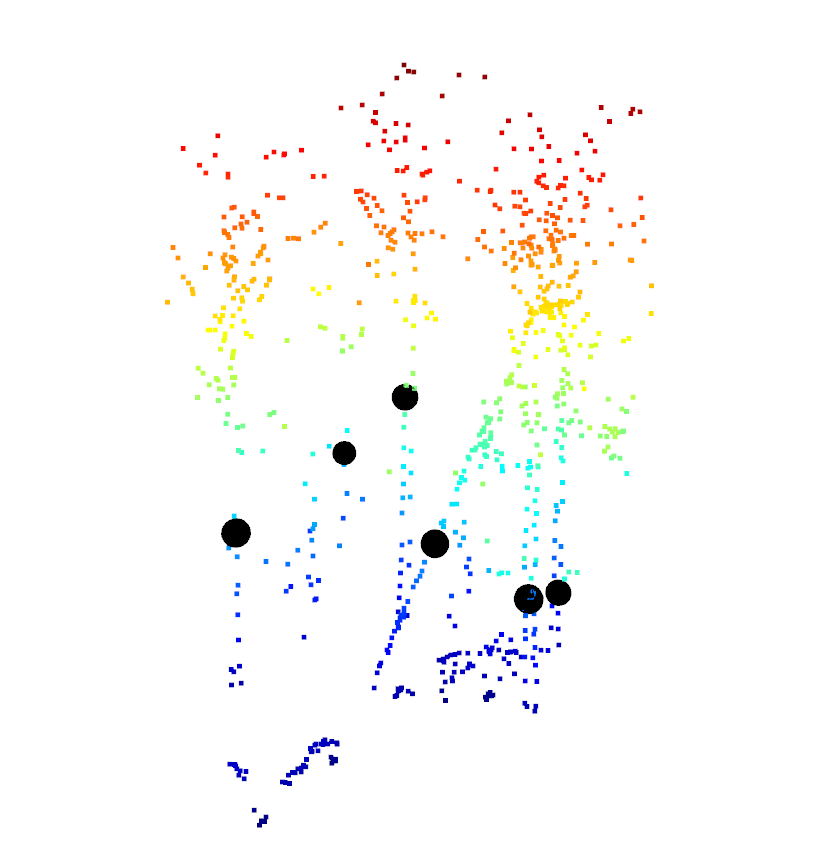
\includegraphics[width=0.9\linewidth]{imaxes/grountCad.png}
    \caption{Ground Truth}
    \label{fig:last3}
  \end{subfigure}
  
  \caption{Ejemplo de Detección en Caducifolios}
  \label{fig:algo2}
\end{figure}


\begin{figure}
  \begin{subfigure}{0.5\textwidth}
    \centering
    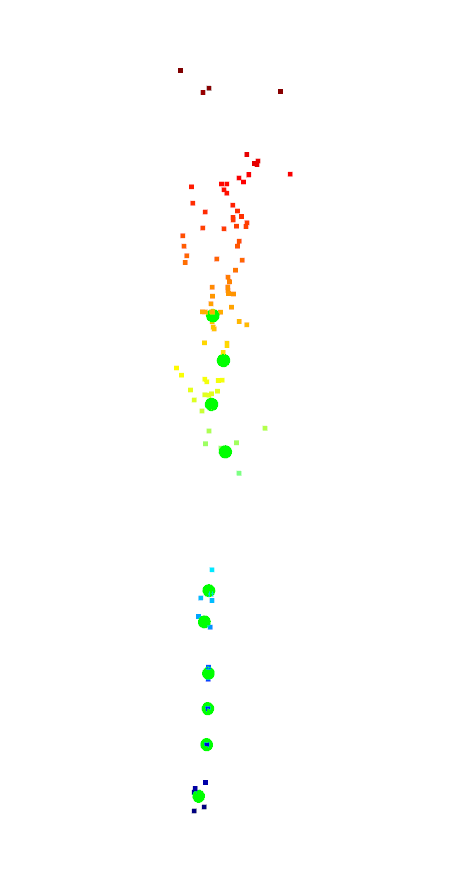
\includegraphics[width=0.8\linewidth,height=0.9\linewidth]{imaxes/centroidesCad1.png}
    \label{fig:last1}
  \end{subfigure}%
  \begin{subfigure}{0.5\textwidth}
    \centering
    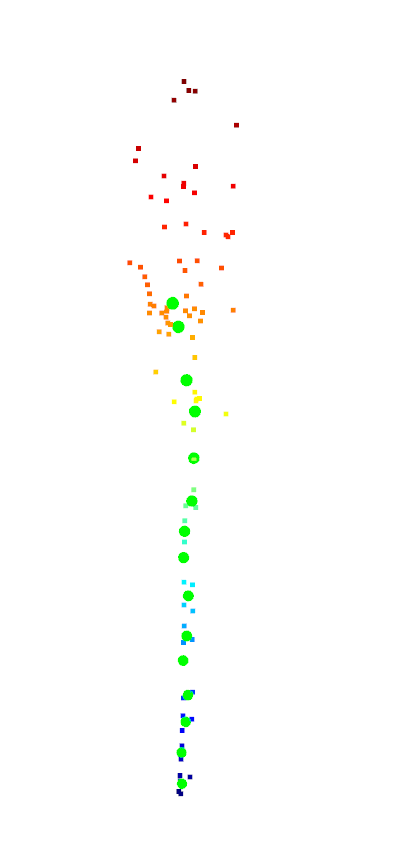
\includegraphics[width=0.8\linewidth,height=0.9\linewidth]{imaxes/centroidesCad2.png}
    \label{fig:last}
  \end{subfigure}
 \caption{Ejemplo de los centroides que forman una linea para caducifolios}
  \label{fig:algo2}
\end{figure}
%\include{contido/...}
 \chapter{Conclusións}
\label{chap:conclusions}

\lettrine{E}{n} este ultimo capitulo se expondrán las conclusiones obtenidas tras realizar este proyecto y los aprendizajes realizados. También Comentaremos que posibles lineas de futuro se podrían seguir para mejorar el trabajo realizado hasta ahora.

\section{Conclusiones}


\section{Trabajo Futuro}
En este proyecto, se emplearon técnicas geométricas para determinar la presencia de árboles. Durante la fase inicial, se consideró la utilización de una red neuronal como \textit{PointNet} \cite{pointnet} para esta tarea. Sin embargo, esta aproximación presentaba un desafío en términos de la necesidad de una amplia y diversa base de datos de miles de árboles de distintas especies, con el fin de asegurar la robustez del sistema. Debido a los plazos ajustados del proyecto, se optó por descartar esta opción.

En relación al rendimiento del código desarrollado, una mejora potencial consistiría en lograr compatibilidad con librerías GPU como \textit{CUDA} o \textit{OpenCL}. Esto permitiría aprovechar la capacidad de procesamiento gráfico para ejecutar en paralelo las numerosas operaciones necesarias en el procesamiento de nubes de puntos. Otra forma de ganar rendimiento seria portar el código a Rust un lenguaje mucho mas rápido y eficiente que Python.

 %%%%%%%%%%%%%%%%%%%%%%%%%%%%%%%%%%%%%%%%
 % Apéndices, glosarios e bibliografía  %
 %%%%%%%%%%%%%%%%%%%%%%%%%%%%%%%%%%%%%%%%

 %\appendix
 %\appendixpage
 %\chapter{Material adicional}
\label{chap:adicional}

\lettrine{E}{xemplo} de capítulo con formato de apéndice, onde se pode
incluír material adicional que non teña cabida no corpo principal do
documento, suxeito á limitación de 80 páxinas establecida no
regulamento de TFGs.


%\include{anexos/...}

 \printglossary[type=\acronymtype,title=\nomeglosarioacronimos]
 \printglossary[title=\nomeglosariotermos]

 \bibliographystyle{IEEEtranN}
 \bibliography{\bibconfig,bibliografia/bibliografia}
 \clearpage
 
\end{document}

%%%%%%%%%%%%%%%%%%%%%%%%%%%%%%%%%%%%%%%%%%%%%%%%%%%%%%%%%%%%%%%%%%%%%%%%%%%%%%%%
